\documentclass[11pt]{memoir}

\usepackage[margin=1.375in]{geometry}
%\usepackage[protrusion=true,expansion=true]{microtype}

%\usepackage[center]{titlesec}

\usepackage[pdftex,
	    pdftitle={Algebraic topology}]{hyperref}
\usepackage{spectralsequences}

\usepackage{mathtools}
%\usepackage{listings}

\usepackage[T1]{fontenc}

%\usepackage[urw-garamond]{mathdesign}
%\usepackage[left=2in,right=2in,top=2in,bottom=2.5in]{geometry}
%\usepackage[margin=1.25in]{geometry}
%\pagestyle{plain}
%\usepackage{fullpage}

\usepackage{setspace}
%\setstretch{1.1}

\usepackage{todonotes}

\usepackage{amsmath}
%\usepackage{amsfonts}
\usepackage{amssymb}
\usepackage{float}
\usepackage{amsthm}
\usepackage{comment}
%\usepackage{amscd}

%\usepackage{txfonts} % Thanks to Eric for showing me that this font exists.
%%\usepackage{kpfonts}
%\renewcommand{\Top}{\mathbf{Top}}
\newcommand{\Top}{\mathbf{Top}}

\usepackage{color}
\usepackage[all]{xy}
\usepackage{verbatim}

\usepackage[mathscr]{eucal}
\usepackage{graphicx}
\usepackage{tikz-cd}

\usepackage{chngcntr} % to number sections consecutively across chapters

\setcounter{chapter}{3}
\setcounter{section}{38}


\counterwithout{section}{chapter}

\tikzset{%
    symbol/.style={%
        draw=none,
        every to/.append style={%
            edge node={node [sloped, allow upside down, auto=false]{$#1$}}}
    }
}



\theoremstyle{theorem}
\newtheorem{theorem}{Theorem}[section]
\newtheorem{thm-defn}[theorem]{Theorem-Definition}
\newtheorem{prop}[theorem]{Proposition}
\newtheorem{lemma}[theorem]{Lemma}
\newtheorem{corollary}[theorem]{Corollary}

\theoremstyle{definition}
\newtheorem{problem}[theorem]{Problem}
\newtheorem{definition}[theorem]{Definition}
\newtheorem{notation}[theorem]{Notation}
\newtheorem{summary}[theorem]{Summary}
\newtheorem{note}[theorem]{Note}
\newtheorem{claim}[theorem]{Claim}
\newtheorem{exercise}[theorem]{Exercise}
\newtheorem{terminology}[theorem]{Terminology}
\newtheorem{construction}[theorem]{Construction}
%\theoremstyle{remark}
\newtheorem{remark}[theorem]{Remark}
\newtheorem{example}[theorem]{Example}
\newtheorem{question}[theorem]{Question}
\newtheorem{slogan}[theorem]{Slogan}
\newtheorem{warning}[theorem]{Warning}
\newtheorem{solution}[theorem]{Solution}
\newtheorem{property}[theorem]{Property}

\DeclareMathOperator{\Th}{Th}
\DeclareMathOperator{\Aut}{Aut}
\DeclareMathOperator{\coeq}{coeq}
\DeclareMathOperator{\colim}{colim}
\DeclareMathOperator{\coker}{coker}
\DeclareMathOperator{\cone}{cone}
\DeclareMathOperator{\Der}{Der}
\DeclareMathOperator{\Ext}{Ext}
\DeclareMathOperator{\Fun}{Fun}
\DeclareMathOperator{\hocolim}{hocolim}
\DeclareMathOperator{\holim}{holim}
\DeclareMathOperator{\Hom}{Hom}
\DeclareMathOperator{\Iso}{Iso}
\DeclareMathOperator{\img}{im}
\DeclareMathOperator{\Map}{Map}
\DeclareMathOperator{\Tot}{Tot}
\DeclareMathOperator{\Tor}{Tor}
\DeclareMathOperator{\Res}{Res}
\DeclareMathOperator{\Spec}{Spec}
\DeclareMathOperator{\rank}{Rank}
\DeclareMathOperator{\Vect}{Vect}
\DeclareMathOperator{\rla}{\rightleftarrows}
\DeclareMathOperator{\lra}{\leftrightarrows}

\def\llarrow{  \hspace{.05cm}\mbox{\,\put(0,-2){$\leftarrow$}\put(0,2){$\leftarrow$}\hspace{.45cm}}}
\def\rrarrow{  \hspace{.05cm}\mbox{\,\put(0,-2){$\rightarrow$}\put(0,2){$\rightarrow$}\hspace{.45cm}}}
\def\lllarrow{ \hspace{.05cm}\mbox{\,\put(0,-3){$\leftarrow$}\put(0,1){$\leftarrow$}\put(0,5){$\leftarrow$}\hspace{.45cm}}}
\def\rrrarrow{ \hspace{.05cm}\mbox{\,\put(0,-3){$\rightarrow$}\put(0,1){$\rightarrow$}\put(0,5){$\rightarrow$}\hspace{.45cm}}}

\def\cA{\mathcal A}\def\cB{\mathcal B}
\def\cc{\mathcal C}\def\cC{\mathbf C}
\def\cd{\mathcal D}
\def\ce{\mathcal E}\def\cf{\mathcal F}\def\cG{\mathcal G}\def\cH{\mathcal H}
\def\cI{\mathcal I}\def\cJ{\mathcal J}\def\cK{\mathcal K}\def\cL{\mathcal L}
\def\cM{\mathcal M}\def\cN{\mathcal N}\def\cO{\mathbf O}\def\cP{\mathcal P}
\def\cQ{\mathcal Q}\def\cR{\mathcal R}\def\cS{\mathcal S}\def\cT{\mathcal T}
\def\cU{\mathcal U}\def\cV{\mathcal V}\def\cW{\mathcal W}\def\cX{\mathcal X}
\def\cY{\mathcal Y}\def\cZ{\mathcal Z}

\def\AA{\mathbb A}\def\BB{\mathbb B}\def\CC{\mathbf C}\def\DD{\mathbb D}
\def\EE{\mathbb E}\def\FF{\mathbf F}\def\GG{\mathbb G}\def\HH{\mathbf H}
\def\II{\mathbb I}\def\JJ{\mathbb J}\def\KK{\mathbb K}\def\LL{\mathbb L}
\def\MM{\mathcal M}\def\NN{\mathbb N}\def\OO{\mathbb O}\def\PP{\mathbf P}
\def\QQ{\mathbf Q}\def\RR{\mathbf R}\def\SS{\mathbb S}\def\TT{\mathbb T}
\def\UU{\mathbb U}\def\VV{\mathbb V}\def\WW{\mathbb W}\def\XX{\mathbb X}
\def\YY{\mathbb Y}\def\ZZ{\mathbf Z}

\usepackage{amsbsy}

\newcommand{\CP}{\mathbf{CP}}
\newcommand{\RP}{\mathbf{RP}}
\newcommand{\Set}{\mathbf{Set}}
\newcommand{\Gra}{\mathrm{Gr}}
\newcommand{\GL}{\mathrm{GL}}
\newcommand{\gl}{\mathit{gl}}

\newcommand{\nn}{\nonumber}
\newcommand{\nid}{\noindent}
\newcommand{\ra}{\rightarrow}
\newcommand{\la}{\leftarrow}
\newcommand{\xra}{\xrightarrow}
\newcommand{\xla}{\xleftarrow}

\newcommand{\weq}{\xrightarrow{\sim}}
\newcommand{\cofib}{\rightarrowtail}
\newcommand{\fib}{\twoheadrightarrow}
%\newcommand{\cofib}{\to}
%\newcommand{\fib}{\to}

\newcommand\cHH{\check{H}}
\newcommand{\Fl}{\mathrm{Fl}}
\newcommand{\Fr}{\mathrm{Fr}}
\newcommand\cCC{\check{C}}
\newcommand{\MFGL}{\mathcal M_{\mathit{FGL}}}
\newcommand{\calO}{{\mathcal O}}
\newcommand{\calC}{{\mathcal C}}
\newcommand{\set}{{\mathrm{Set}}}
\newcommand{\Deltab}{{\mathbf{\Delta}}} 
%change this to bold Delta. This is like this
%here because garamond messes up bold things.
\newcommand{\spec}{\mathrm{Spec}}
\newcommand{\Z}{\mathbf Z}
\newcommand{\Sin}{\mathrm{Sin}}
\newcommand{\htop}{\mathrm{Ho}(\mathbf{Top})}
\newcommand{\sca}{\mathcal{A}}
\DeclareMathOperator{\Spf}{Spf}
\newcommand{\CG}{\mathbf{CG}}
\newcommand{\Ab}{\mathbf{Ab}}
\newcommand{\Bun}{\mathrm{Bun}}
\newcommand{\Ho}{\mathrm{Ho}}
\newcommand{\gr}{\mathrm{gr}}
\newcommand{\sk}{\mathrm{sk}}
\newcommand{\Cat}{\mathbf{Cat}}
\newcommand{\wt}[1]{\widetilde{{#1}}}
\newcommand{\xar}[1]{\xrightarrow{{#1}}}
\newcommand{\pr}{\mathrm{pr}}
\newcommand{\ev}{\mathrm{ev}}
\newcommand{\inc}{\mathrm{in}}
\newcommand{\Spin}{\mathrm{Spin}}
\newcommand{\String}{\mathrm{String}}
\newcommand{\Sk}{\mathrm{Sk}}
\newcommand{\Gp}{\mathbf{Gp}}


\newcommand{\downsubseteq}{\mathbin{\rotatebox[origin=c]{-90}{$\subseteq$}}}

% for pullback and pushout squares
\usepackage{pigpen}
\newcommand{\po}{\ar@{}[dr]|{\text{\pigpenfont R}}}
\newcommand{\pb}{\ar@{}[dr]|{\text{\pigpenfont J}}}
%%%%%%%%%%%%%%%%

%\usepackage{ebgaramond}
%\usepackage{fancyhdr}
% 
%\newcommand{\myheader}{
%    \ifnum\value{section} > 38
%    18.906
%    \else
%    18.905
%    \fi
%}
%
%\pagestyle{fancy}
%\fancyhf{}
%\fancyhead[LE]{Notes by Sanath Devalapurkar}
%\fancyhead[LO]{Taught by Haynes Miller}
%\chead{Notes for \myheader}
%\rhead{Lecture \thesection}
%\cfoot{\thepage}

%\usepackage[urw-garamond]{mathdesign}

\begin{document}
\title{Algebraic Topology}
\author{Lectures by Haynes Miller\\
Notes based on live{\TeX}ed record made by Sanath Devalapurkar\\
Images created by John Ni
}
%\date{Fall 2016 -- Spring 2017}

\frontmatter

\maketitle

\section{Preface}



Here is an overview of this part of the book.
\begin{enumerate}
    \item \textbf{General homotopy theory.} This includes category theory;
	because it started as a part of algebraic topology, we'll speak freely
	about it here.  We'll also cover the general theory of homotopy groups,
	long exact sequences, and obstruction theory.
    \item \textbf{Bundles.} One of the major themes of this part of the book is
	the use of bundles to understand spaces.  This will include the theory
	of classifying spaces; later, we will touch upon connections with
	cohomology.
    \item \textbf{Spectral sequences.} It is impossible to describe everything
	about spectral sequences in the duration of a single course, so we will
	focus on a special (and important) example: the Serre spectral
	sequence.  As a consequence, we will derive some homotopy-theoretic
	applications.  For instance, we will relate homotopy and homology (via
	the Hurewicz theorem, Whitehead's theorem, and ``local'' versions like
	Serre's mod C theory).
    \item \textbf{Characteristic classes.} This relates the geometric theory of
	bundles to algebraic constructions like cohomology described earlier in
	the book.  We will discuss many examples of characteristic classes,
	including the Thom, Euler, Chern, and Stiefel-Whitney classes.  This
	will allow us to apply a lot of the theory we built up to geometry.

\end{enumerate}

\newpage
\tableofcontents
\newpage

\mainmatter

%\part{18.906 -- homotopy theory}\label{906}

\chapter{Basic homotopy theory}
\section{Limits, colimits, and adjunctions}\label{906}

\subsection{Limits and colimits}

I want to begin by developing a little more category theory.

\begin{definition}
Suppose $\cI$ is a small category (so that it has a \emph{set} of objects),
and let $\cc$ be another category.  Let $X:\cI\to\cc$ be a functor.
    A \emph{cone under $X$} is a natural transformation $\eta$ from $X$ to a constant functor; to be explicit, this means that for every object $i$ of $\cI$
we  have a map $\eta_i: X_i\to Y$, and these maps are compatible in the sense 
that for every $f:i\to j$ in $\cI$ the following diagram commutes:
    \begin{equation*}
	\xymatrix{
	    X_i\ar[d]^{f_\ast}\ar[r]^{\eta_i} & Y \ar[d]^= \\
	    X_j\ar[r]^{\eta_j} & Y\,.
	    }
    \end{equation*}
    A \emph{colimit} of $X$ is an initial cone $(L,\tau_i)$ under $X$; to be 
    explicit, this means that for any cone $(Y,\eta_i)$ under $X$,
    there exists a unique map $h:L\to Y$ such that $h\circ \tau_i = \eta_i$
for all $i$.
\end{definition}
As with any universal property, any two colimits are isomorphic by a unique
isomorphism; but existence is another matter. Also, 
as always for category theoretic concepts, some examples are in order.
\begin{example}\label{coproductsarecolimits}
    If $\cI$ is a discrete category (that is, the only maps are identity maps;
$\cI$ is entirely determined by its set of objects), 
the colimit of a functor $\cI\to\cc$
    is the coproduct in $\cc$ (if this coproduct exists!).
\end{example}
\begin{example}
In Lecture 23 we discussed directed posets and the direct limit of a directed 
system 
$X:\cI\to\cc$. The colimit simply generalizes this to arbitrary
indexing categories rather than restricting to directed partially 
ordered sets. 
\end{example}
\begin{example}\label{colimitgroupaction}
    Let $G$ be a group; we can view this as a category with one object, where the morphisms are the elements of the group and composition is given by the group structure.
    If $\cc = \Top$ is the category of topological spaces, a functor $G\to \cc$ is simply a
    group action on a topological space $X$.
    The colimit of this functor is the orbit space of the $G$-action on $X$.
\end{example}
\begin{example}
    Let $\cI$ be the category whose objects and morphisms are determined by the following directed graph:
    \begin{equation*}
	\xymatrix{ & a\ar[dl]\ar[dr] & \\
	b & & c.}
    \end{equation*}
    The colimit of a diagram $\cI\to \cc$ is called a \emph{pushout}.
With  $\cc=\Top$, again, a functor $\cI\to \cc$ is determined by a diagram of spaces:
    \begin{equation*}
	\xymatrix{
	    & A\ar[dl]_f\ar[dr]^g & \\
	    B & & C.
	    }
    \end{equation*}
    The colimit of such a functor is just the pushout $B\cup_A C:= B\sqcup C/\sim$, where $f(a)\sim g(a)$ for all $a\in A$.
    We have already seen this in action before: a special case of this construction appears in the process of attaching cells to build up a CW-complex.

    If $\cc$ is the category of groups, instead, the colimit of such a functor is the free product quotiented out
    by a certain relation; this is called the \emph{amalgamated free product}.
\end{example}
\begin{example}
    Suppose $\cI$ is the category defined by the following directed graph:
\begin{equation*}
    \begin{tikzcd}
	a\ar[r,shift left=.75ex]\ar[r,shift right=.75ex] & b.
    \end{tikzcd}
\end{equation*}
    The colimit of a diagram $\cI\to\cc$ is called the \emph{coequalizer} of the diagram. If $\cc=\Set$, the coequalizer of $f,g:A\rightrightarrows B$ is the 
quotient of $B$ by the equivalence relation generated by $f(a)\sim g(a)$ for
$a\in A$.
\end{example}

    One can also consider cones \emph{over} a diagram $X:\cI\to\cc$: this is simply a cone in the opposite category.
\begin{definition}
The \emph{limit} of a diagram $X:\cI\to\cc$ is a terminal object in cones over $X$.
\end{definition}

\begin{exercise}
    Revisit the examples provided above: what is the limit of each diagram?
For instance, a product is a limit over a discrete category, 
and the limit of the diagram described in Example \ref{colimitgroupaction} is just the fixed points.
\end{exercise}

\subsection{Adjoint functors}
The notion of a colimit as a special case of the more general concept of an 
adjoint functor, as long as we are dealing with a cocomplete category as in
the following definition.
\begin{definition}
    A category $\cc$ is \emph{cocomplete} if all functors from small categories to $\cc$ have colimits.
    Similarly,  $\cc$ is \emph{complete} if all functors from small categories
to $\cc$ have limits. 
\end{definition}
All examples considered above are both cocomplete and complete.

Let's write $\cc^\cI$ for the category of functors from $\cI$ to $\cc$,
and natural transformations between them.


There is a functor $c:\cc\to \cc^\cI$, given by sending any object to the constant functor taking on that value.
The process of taking the colimit of a diagram supplies us with a functor 
$\colim_{\cI}:\cc^\cI\to \cc$.
We can characterize this functor via the formula
\[
\cc(\colim{}_{i\in \cI} X_i,Y) = \cc^\cI(X,c_Y)\,,
\]
where $X$ is any functor from $\cI$ to $\cc$, $Y$ is any object of $\cc$,
and $c_Y$ denotes the constant functor with value $Y$.
This formula is reminiscent of the adjunction operator in linear algebra,
and is in fact our first example of an adjunction.

\begin{definition}
    Let $\cc,\cd$ be categories, and suppose given functors 
$F:\cc\to \cd$ and $G:\cd\to\cc$.
    An \emph{adjunction between $F$ and $G$} is an isomorphism:
    $$\cd(FX,Y) = \cc(X,GY),$$
    that is natural in $X$ and $Y$.
    In this situation, we say that $F$ is a \emph{left adjoint} of $G$ and $G$ is a \emph{right adjoint} of $X$.
    %People typically write left adjoints on the top.
\end{definition}
This notion was invented by the late MIT Professor Dan Kan.

We've already seen one example of adjoint functors. Here is another one.
\begin{definition}[Free groups]
    There is a forgetful functor $u:\mathbf{Grp}\to\mathbf{Set}$.
    Any set $X$ gives rise to a group $FX$, the free group on $X$ elements.
    It is determined by a universal property:
    set maps $X\to u\Gamma$ are the same as group maps $FX\to \Gamma$,
    where $\Gamma$ is any group.
    This is exactly saying that the free group functor the left adjoint to the forgetful functor $u$.
\end{definition}
In general, ``free objects'' come from left adjoints to forgetful functors.

As a general notational practice, try to write the left adjoint as the top 
arrow: 
\[
F:\cc\rightleftarrows\cd:G \qquad\hbox{or}\qquad G:\cd\leftrightarrows\cc:F \,.
\]
 



\subsection{The Yoneda lemma}
One of the many important principles in category theory is that an object is determined by the collection of all maps out of it.
The Yoneda lemma is a way of making this precise. Observe that 
for any $X\in\cc$ the association $Y\mapsto\cc(X,Y)$ gives us a functor
$\cc\to\Set$. This functor is said to be {\em corepresentable} by $X$.
Suppose that $G:\cc\to\Set$ is any functor. An element $x\in G(X)$ 
determines a natural transformation 
\[
\theta_x:\cc(X,-)\to G
\]
in the following way. Let $Y\in\mathrm{ob}\cc$. Map $\cc(X,Y)\to G(Y)$
by sending $f:X\to Y$ to $f_*(x)\in G(Y)$. 

\begin{lemma}[Yoneda lemma]
The association $x\mapsto\theta_x$ provides a bijection
    $$\mathrm{nt}(\cc(X,-),G)\xrightarrow{\cong}G(X).$$
\end{lemma}
\begin{proof}
The inverse is given as follows: Send a natural transformation 
$\theta:C(X,-)\to G$ to $\theta_X(1_X)\in G(X)$. 
\end{proof}
In particular, if $G$ is also corepresentable -- $G=\cc(Y,-)$, say --
then 
\[
\mathrm{nt}(\cc(X,-),\cc(Y,-))\cong \cc(Y,X)\,.
\]
Simply put, natural transformations $\cc(X,-)\to \cc(Y,-)$ are in natural
bijection with maps $Y\to X$. Consequently natural isomorphisms 
$\cc(X,-)\xrightarrow{\cong}\cc(Y,-)$ are in natural bijection with 
isomorphims $Y\xrightarrow{\cong}X$. 
So, for example, the object that corepresents a corepresentable functor 
is unique up to unique isomorphism.

From the Yoneda lemma, we can obtain some pretty miraculous conclusions.
For instance, functors with left and/or right adjoints are very well-behaved.
\begin{theorem}\label{adjointslimits}
    Let $F:\cc\to\cd$ be a functor.
    If $F$ admits a right adjoint then it preserves colimits.
    Dually, if $F$ admits a left adjoint then it preserves limits.
\end{theorem}
\begin{proof}
    We'll prove the first statement; the dual proof gives the other.
    Let $F:\cc\to\cd$ be a functor that admits a right adjoint $G$, and let $X:\cI\to\cc$ be a
    small $\cI$-indexed diagram in $\cc$. Suppose that the colimit 
$\colim_{\cI}X$ exists. From the definition of colimit, there is
    for any object $Y$ of $\cc$ an isomorphism
$$
\cc(\colim_{\cI} X, Y) \cong \lim{}_{\cI}\cc(X, Y)\,.
$$
   
    Let $Z$ be any object of $\cd$, and note the sequence of natural 
isomorphisms:
    \begin{align*}
	\cd(F(\colim_{\cI} X), Y) & \cong \cc(\colim_{\cI} X, G(Y))\\
	& \cong \lim{}_{\cI}\cc(X, G(Y))\\
	& \cong \lim{}_{\cI}\cd(F(X), Y)\\
	& \cong \cd(\colim_{\cI}F(X), Y).
    \end{align*}
    The Yoneda lemma now finishes the job.
\end{proof}

\section{Cartesian closure and compactly generated spaces}

A lot of homotopy theory is about loop spaces and mapping spaces. 
The compact-open topology is available to us -- and we'll recall it later.
But it suffers from some defects. To clarify how a mapping object
should behave in an ideal world, I want to make another category-theoretical
digression

\begin{definition} Let $\cc$ be a category with finite products. 
It is {\em Cartesian closed} if for any object $X$ in $\cc$, the functor
$X\times-$ has a right adjoint. 
\end{definition}

\begin{example} If $\cc=\Set$, 
\[
\Set(W\times X,Y)=\Set(X,\Set(W,Y))\,,
\]
so the right adjoint is the co-representable functor $\Set(W,-)$. 
\end{example}

So mapping objects are ideally given as the right adjoint to Cartesian
product.

Many otherwise well-behaved categories are not Cartesian-closed. 
The category of abelian groups is an example. There is indeed a functor 
$Y\mapsto\Hom(W,Y)$, for any abelian group $W$; but it is the right adjoint
not of $W\times-$ but rather of $W\otimes-$. 

As a general thing, if a functor has a right adjoint then that right
adjoint is well-defined up to canonical natural isomorphism; so we will
always speak of {\em the} right adjoint. We'll write the right adjoint 
to $X\times-$ using exponential notation,
\[
Y\mapsto Y^W\,,
\]
so that there is a natural bijection
\[
\cc(W\times X,Y)=\cc(X,Y^W)\,.
\]

The category of topological spaces is supposed to behave more like $\Set$
than like $\Ab$, but it turns out that $\Top$ is not Cartesian closed either.
Small modifications of it are, however. We describe them below.

To better understand the consequence of Cartesian closure, it's convenient
to restate the definition of adjointness. So suppose that 
\[
F:\cc\rightleftarrows \cd:G
\]
is an adjoint pair of functors, so that
\[
\cd(FX,Y)=\cc(X,GY)
\]

Take $Y=FX$; the identity $1_{FX}$ corresponds to a map $\eta_X:X\to GFX$,
called the {\em unit} of the adjunction. 

Take $X=GY$; the identity $1_{GY}$ corresponds to a map $\epsilon_Y:FGY\to Y$,
called the {\em counit} of the adjunction.

Both these maps are natural transformations of endofunctors of $\cc$. 

\begin{example} Take for example the free group adjunction
\[
F:\Set\rightleftarrows\Gp:u\,.
\]
In this case, $\eta:X\to uFX$ sends a set to itself inside the free group
it generates; and $\epsilon:FuY\to Y$ sends a word in the free group on
the set underlying $Y$ to the product of those elements in $Y$. 
\end{example}

\begin{lemma} The unit and counit of an adjunction make the following
diagrams commute.
\[
\xymatrix{
GFGY \ar[r]^{G\epsilon_Y} & GY & & FGFX \ar[r]^{\epsilon_{FX}} & FX \\
GY \ar[u]^{\eta_{GY}} \ar[ur]_= & & & FX \ar[u]^{F\eta_X} \ar[ur]_=
}
\]
Conversely, equipping functors $F$ and $G$ with natural 
transformations $\eta$ and $\epsilon$ making these diagrams commute 
establishs $(F,G)$ as an adjoint pair.
\end{lemma}

In the Cartesian setting, then, we have natural transformations
\[
\eta_X:X\to(W\times X)^W\,,\quad \epsilon_Y:W\times Y^W\to Y\,.
\]
In case $\cc=\Set$, these are given by
\[
x\mapsto(w\mapsto(w,x))\,,\quad(w,f)\mapsto f(w)\,,
\]
that is, including a slice and evaluation. You should check that the 
two triangles commute in this case! 

Here are some direct consequences of Cartesian closure. Note: the assumption
that finite products exist in $\cc$ includes the case of the empty product,
which is a terminal object $*$.

\begin{prop}
Let $\cc$ be Cartesian closed. \\
(1) $(X,Z)\mapsto Z^X$ is a functor $\cc^{op}\times\cc\to\cc$.\\
(2) $\cc(X,Y)=\cc(*,Y^X)$.\\
(3) $X\times-$ commutes with all colimits.
\end{prop}

\subsection{CGHW spaces}\label{CGWHspaces}

The last Proposition shows that $\Top$ is not Cartesian closed:
A standard example from general topology shows that if $Y\to Z$ is a
quotient map, the induced map $X\times Y\to X\times Z$ may fail to be
a quotient map. But any quotient maps are precisely coequalizers in $\Top$. 

Henry Whitehead showed that crossing with a compact Hausdorff space
{\em does} preserve quotient maps. This will often suffice, but often not, 
and the convenience of working in a Cartesian closed category is compelling. 

Inspired by Whitehead's theorem, we agree to accept only properties of a space
that can be observed by mapping compact Hausdorff spaces into it. 

\begin{definition}
    Let $X$ be a space.
    A subspace $F\subseteq X$ is said to be \emph{compactly closed} if,
    for any map $k:K\to X$ from a compact Hausdorff space $K$, 
    the preimage $k^{-1}(F)\subseteq K$ is closed.
\end{definition}
It is clear that any closed subset is compactly closed, but
there might be compactly closed sets which are not closed in the topology 
on $X$. This motivates the definition of a $k$-space:
\begin{definition}
    A topological space $X$ is said to be a \emph{$k$-space}
    if every compactly closed set is closed.
\end{definition}
The $k$ comes either from ``kompact'' and/or the general topologist 
John Kelley.

A more categorical characterization of this property is: 
$X$ is a $k$-space if and only if
a map $X\to Y$ is continuous precisely when for every compact Hausdorff space $K$ and map $k:K\to X$ the composite $K\to X\to Y$ is continuous.
For instance, compact Hausdorff spaces are $k$-spaces. First countable (so metric spaces) and CW-complexes are also $k$-spaces.

While not all topological spaces are $k$-spaces, any space can be 
``$k$-ified.''
The procedure is simple: endow the underlying set of a space $X$ with 
the topology consisting of all compactly closed sets.
The reader should check that this is indeed a topology on $X$.
The resulting topological space is denoted $kX$.
This construction immediately implies, for instance, that the identity 
$kX\to X$ is continuous, and is the terminal map to $X$ from a $k$-space.

Let $k\Top$ be the category of $k$-spaces.
This is a subcategory of the category of topological spaces, and we will write
$i:k\Top\hookrightarrow \Top$ for the inclusion functor.
The process of $k$-ification gives a functor $\Top\to k\Top$, which has the property that
$$k\Top(X,kY)=\Top(iX,Y)\,.$$
This is another example of an adjunction!
In this case the counit $kiX\to X$ is a homeomorphism.
We can conclude from this that the product in $k\Top$ may be computed as 
\[
X\times^{k\Top}Y=k(iX\times iY)\,.
\]

The category $k\Top$ has good categorical properties inherited from $\Top$:
it is a complete and cocomplete category.
As we will now explain, this category has even better categorical properties
than $\Top$ does.

\subsection{Mapping spaces}\label{mappingspaces}
Let $X$ and $Y$ be topological spaces.
The set $\Top(X,Y)$ of continuous maps from $X$ to $Y$ admits an
interesting topology, the {\em compact-open topology}.
If $X$ and $Y$ are $k$-spaces, we can make a slight modification:
Start with topology on $k\Top(X,Y)$ generated by the sets $W(k,U)$,
where $k:K\to X$ is a map from a compact Hausdorff space and $U\subseteq Y$
is open, defined by
\[
W(k,U) = \{f:X\to Y: f(k(K))\subseteq U\}\,.
\]
This topology is probably not itself determined by maps from compact
Hausdorff spaces, so $k$-ify it. 
We write $Y^X$ for the resulting $k$-space; its underlying
set is still the set of continuous maps from $X$ to $Y$. With this definition,
we have:
\begin{prop}
The category $k\Top$ is Cartesian closed.
\end{prop}
\begin{proof}
See \cite[Proposition 2.11]{StricklandCGWH}.
\end{proof}


\section{Weak Hausdorff, Basepoints}\label{basepoints}
The ancients came up with a good definition of a topology ---
but $k$-spaces are better!
Sometimes, though, we can be greedy and ask for even more:
for instance, we can demand a Hausdorff condition.
This leads to a further refinement of $k$-spaces. But ``Hausdorff'' isn't
quite the appropriate condition in the context of $k$-spaces. Rather: 

\begin{definition}
    A space $X$ is {\em weak Hausdorff} if the image of every continuous 
map $K\to X$ from a compact Hausdorff space $K$ is closed.
\end{definition}
Another way to say this is that the map itself if closed. Clearly Hausdorff implies weak Hausdorff. Every singleton subset of a weak Hausdorff space is 
closed (since the one-point space is compact Hausdorff).
\begin{prop}
    Let $X$ be a $k$-space.
    \begin{enumerate}
	\item $X$ is weak Hausdorff if and only if 
$\Delta:X\to X\times^{k\Top}X$ is closed.
(In algebraic geometry such a condition is termed {\em separated}.)
	\item Let $R\subseteq X\times X$ be an equivalence relation. If $R$ is closed, then $X/R$ is weak Hausdorff.
    \end{enumerate}
\end{prop}
\begin{definition}
    A space is {\em compactly generated} if it is weak Hausdorff and a
$k$-space. The category of such spaces is written $\CG$.
\end{definition}
We have a pair of adjoint pairs:
\[
\Top\,\underset{k}{\overset{i}{\lra}}\,k\Top\,
\underset{j}{\overset{h}{\rla}}\,\CG
\]
so 
\[
ikX\to X \quad,\qquad hjZ\xrightarrow{\cong}Z \,,
\]
\[
Y\xrightarrow{\cong}kiY \quad,\qquad Y\to jhY\,.
\]
The functor $h$ is defined by dividing $Y$ by the intersection of all closed
equivalence relations on it. $k$-ification is a right adjoint, but 
weak Hausdorfification, being formation of a quotient, is a left adjoint.
The dangerous and annoying feature of $h$ is that if $Y$ is not weak Hausdorff 
then the map $Y\to jhY$ is not a bijection; the underlying point-set changes. 


\begin{lemma} If $Y$ is a $k$-space and $Z$ is weak Hausdorff, then $Z^Y$ is
weak Hausdorff.
\end{lemma}

\begin{corollary}
The category $\CG$ is Cartesian closed.
\end{corollary}

We will essentially always be working with either $k\Top$ or $\CG$; 
most of the time either one will do. I will just call the objects ``spaces,''
and (I'm sorry) write $\Top$ for the corresponding category.

Here's an example of how useful the formation of mapping spaces can be. 
We already know that a {\em homotopy} between maps $f,g:X\to Y$ is a map 
$h:I\times X\to Y$ such that the following diagram commutes.
\begin{equation*}
    \xymatrix{
X\ar[d]_{\inc_0}\ar[dr]^f & &\\
I\times X\ar[r]^h & Y\\
X\ar[u]^{\inc_1}\ar[ur]_g & &
    }
\end{equation*}
We write $f\sim g$ to indicate that $f$ and $g$ are homotopic. This is an
equivalence relation on $\Top(X,Y)$, and 
we define 
\[
[X,Y]=\Top(X,Y)/\sim\,.
\]

The maps $f$ and $g$ are points in the space $Y^X$, and the homotopy $h$ 
is the same thing as a path $\hat f:I\to Y^X$ from $f$ to $g$. So
\[
[X,Y]=\pi_0(Y^X)\,.
\]

To talk about the fundamental group, and higher homotopy groups, using
this strategy, we have to get basepoints into the picture.

\subsection{Basepoints}
A {\em pointed space} is a space $X$ together with a specified ``point'' 
in it, with default notation $*$. The point $\ast$ is called the 
{\em basepoint}. This leads some people refer to ``based spaces,'' but 
to my ear this makes it sound as if we are doing chemistry, or worse, 
and I prefer ``pointed.'' 
 
This gives a category $\Top_\ast$ where the morphisms respect the basepoints. 
This category is complete and cocomplete. For example
\[
(X,\ast)\times (Y,\ast)=(X\times Y,(\ast,\ast))
\]
(where of course I mean to be taking the product in $k\Top$ or $\CG$).
The coproduct is not disjoint union; which basepoint would you pick? So you
identify the two basepoints, to get the ``wedge'' (or in TeX, $\backslash$vee)
\[
X\vee Y=X\sqcup Y/\ast_X\sim \ast_Y\,.
\]

The one-point space $\ast$ is the terminal object in $\Top_*$, as in $\Top$, 
but it is also {\em initial} in $\Top_*$: 
there is exactly one map of pointed spaces from it to 
any $(X,\ast)$. We have a {\em pointed category}: 
A category with initial and terminal objects such that the 
unique map from the first to the second is an isomorphism.

Pointed categories are (almost) never Cartesian closed: for, as we saw,
in a Cartesian closed category $\cc$, $\cc(X,Y)=\cc(\ast,Y^X)$, and
in a pointed category this is a singleton.

But we still know what we would like to take as a ``mapping object'' 
in $\Top_*$:
Define $Y^X_*$ to be the subspace of $Y^X$ consisting of the pointed maps. 
As a replacement for Cartesian closure, 
let's ask: For fixed $X\in\Top_*$, 
does the functor $Y\mapsto Y^X_\ast$ have a left adjoint? 
This would be an analogue in $\Top_*$ of the functor $A\otimes-$ in $\Ab$. 
Compute:
\[
\xymatrix{
\Top(W,Y^X) \ar@{}[rr]|{=} && \{f:X\times W\to Y\} \\
\Top(W,Y_*^X) \ar@{}[rr]|{=} \ar[u]^\subseteq && 
\{f(*,w)=* \,\,\,\forall \,w\in W\} \ar[u]^\subseteq \\
\Top_*(W,Y_*^X) \ar@{}[rr]|{=} \ar[u]^\subseteq && 
{\left\{\begin{array}{ll}
f(*,w)=*&\forall\,w\in W\\
f(x,*)=*&\forall\,x\in X\end{array}\right\}}
\ar[u]^\subseteq 
}
\]
So the map $X\times W\to Y$ corresponding to $f:W\to Y_*^X$ sends the 
wedge $X\vee W\subseteq X\times W$ to the basepoint of $Y$, and hence
factors through the {\em smash product}
\[
X\wedge W=X\times W/X\vee W
\]
obtained by pinching the ``axes'' in the product to a point. We have an
adjoint pair 
\[
X\wedge-:\Top_*\rightleftarrows\Top_*:(-)^X_*\,.
\]

You are invited to check the various properties enjoyed by the smash product,
analogous to properties of the tensor product. So it's functorial in both
variables; the two-point pointed space serves as a unit; and it is associative
and commutative. Associativity is a blessing bestowed by assuming compact
generation; notice that in forming it we are mixing limits (the product)
with colimits (the quotient by the axes), and indeed the smash product
turns out {\em not} to be associative in the full category of spaces. 

Based spaces and all spaces are related by another adjoint pair, 
\[
(-)_+:\Top\rightleftarrows\Top_*:u
\]
where $u$ forgets the basepoint and $(-)_+$ adjoins a disjoint base point. 
The two-point pointed space is then $*_+$, but everyone writes it as $S^0$. 
Explain why this is a reasonable symbol for this pointed space. 


\section{Fiber bundles, fibrations, cofibrations}
\subsection{Fiber bundles}
\begin{definition}\label{fiberbundle}
    A {\em fiber bundle} is a map $p:E\to B$,
    such that for every $b\in B$, there exists
an open subset $U\subseteq B$ containing $b$ and
a map $p^{-1}(U)\to p^{-1}(b)$ such that $p^{-1}(U)\to U\times p^{-1}(b)$ is a homeomorphism.
\end{definition}    
When $p:E\to B$ is a fiber bundle, $E$ is called the \emph{total space}, 
$B$ the \emph{base space}, and $p$ the \emph{projection}.
The point pre-image $p^{-1}(b)\subseteq$ for $b\in B$ is the 
the \emph{fiber over $b$}.

Here is an equivalent way of stating Definition \ref{fiberbundle}:
there is an open cover $\cU$ (a ``trivializing cover'') of $B$
such that for every $U\in\cU$
there is a space $F$ and a homeomorphism
$p^{-1}(U)\simeq U\times F$ that is compatible with the projections 
down to $U$.

A trivial example of a fiber bundle is a product projection. Such fiber 
bundles are in fact called {\em trivial fiber bundles}, and the definition
says that a fiber bundle is a map that is locally (in the base) a trivial
fiber bundle. 

Fiber bundles are naturally occurring objects.
For instance, a covering space $E\to B$ is precisely 
a fiber bundle with discrete fibers. 
\begin{example}[The Hopf fibration]
    The ``Hopf fibration'' provides a beautiful example of a fiber bundle.
    Let $S^3\subset \cC^2$ be the $3$-sphere.
    There is a map $p:S^3\to \CP^1 \cong S^2$ that is given by sending a vector $v$ to the
    complex line through $v$ and the origin.
    This is a non-nullhomotopic map, and is a fiber bundle whose fiber is $S^1$.
    
    Here is another way of thinking of the Hopf fibration.
    Recall that $S^3 = SU(2)$; this contains as a subgroup
    the collection of matrices $\begin{pmatrix}\lambda & \\ & \lambda^{-1}\end{pmatrix}$.
	This subgroup is simply $S^1$, which acts on $S^3$ by translation; 
	the orbit projection is the Hopf fibration is $p$.
\end{example}
The Hopf fibration is a map between smooth manifolds.
A theorem of Ehresmann's says that it is not too hard to check the fiber bundle
condition for a map between smooth manifolds. 
\begin{theorem}[Ehresmann]
    Suppose $E$ and $B$ are smooth manifolds, and let $p:E\to B$ be a smooth (i.e., $C^\infty$) map.
    Then $p$ is a fiber bundle if $p$ is a {\emph proper} (preimages of compact
sets are compact)
\emph{submersion} (that is, $dp:T_e E\to T_{p(e)} B$ is a surjection for all $e\in E$).
\end{theorem}
Much of this course will consist of a study of fiber bundles through 
various essentially algebraic lenses. To bring them into play, we will 
always require a further condition on our bundles. 
\begin{definition}\label{numerable}
An open cover $\cU$ of a space  $X$  is \emph{numerable}
    if there exists a subordinate partition of unity; i.e.,
    there is a family of functions $f_U:X\to [0,1]=I$, indexed by the
elements of $\cU$, such that $f^{-1}((0,1]) = U$
    and any $x\in X$ belongs to only finitely many $U\in\cU$.
    The space $X$ is \emph{paracompact} if any open cover admits a numerable refinement.
    A fiber bundle is \emph{numerable} if it admits a numerable trivializing cover.
\end{definition}
So any fiber bundle over a paracompact space is numerable. 
This isn't too restrictive for us:
\begin{prop}
CW-complexes are paracompact.
\end{prop}

\subsection{Fibrations and path liftings}
During the 1940s and '50's, much effort was devoted to extracting 
homotopy-theoretic features of fiber bundles. It came to be understood
that these consequences relied entirely on a ``homotopy lifting property.''
One of the revolutions in topology around 1960 was the realization that
it was adantageous to take that property as a {\em definition}.
This extension of the notion of a fiber bundle included 
wonderful new examples, but still retained the homotopy theoretic 
consequences. Here is the definition. 
\begin{definition}\label{fibration}
    A {\em (Hurewicz) fibration} is a map $p:E\to B$ that satisfies the
    \emph{homotopy lifting property} (commonly abbreviated as HLP):
Given any $f:W\to E$ and any homotopy $h:I\times W\to B$ with 
$h(0,w)=pf(w)$, there is a map $\overline{h}$ that lifts $h$ and extends $f$:
that is, making the following diagram commute. 
    \begin{equation}\label{hlp}
	\xymatrix{
	    W\ar[r]^f\ar[d]_{\mathrm{in}_0} & E\ar[d]^p\\
	    I\times W\ar[r]_h\ar@{-->}[ur]^{\overline{h}} & B,
	    }
    \end{equation}
\end{definition}
At first sight, this seems like an alarming definition, since
the HLP has to be checked for \emph{all} spaces, \emph{all} maps, and \emph{all} homotopies! 
The HLP is not impossible to check, though.

\begin{exercise}\label{productfibration}
    Check that the projection $\mathrm{pr}_1: B\times F\to B$ is a fibration.
\end{exercise}

\begin{exercise}
Check that the class of fibrations is closed under the following operations.
     \begin{itemize}
	\item Base change: If $p:E\to B$ is a fibration and $X\to B$ is any map, then the induced map $E\times_B X\to X$ is again a fibration.
	\item Products: If $p_i:E_i\to B_i$ 
is a family of fibrations then the product map $\prod p_i$ is again a 
fibration.
\item Exponentiation: If $p:E\to B$ is a fibration and $A$ is any space,
then $E^A\to B^A$ is again fibration.
	\item Composition: If $p:E\to B$ and $q:B\to X$ are both fibrations,
then the composite $qp:E\to X$ is again a fibration.
    \end{itemize}
\end{exercise}

\begin{exercise}
    Let $p:E_0 \to B_0$ be a fibration, and let $f:B \to B_0$ be a homotopy equivalence.
    Prove that the induced map $B\times_{B_0} E_0 \to E_0$ is a homotopy equivalence.
    (Warning: this exercise has a lot of technical details!) 
\end{exercise}


There is a simple geometric interpretation of what it means for a map to be a fibration, in terms of ``path liftings''. We'll use Cartesian closure! 
The adjoint of the solid arrow part of \eqref{hlp} is
\begin{equation}\label{hlp2}
    \xymatrix{
	E\ar[r]^p & B\\
	W\ar[u]^f\ar[r]_{\widehat{h}} & B^I\ar[u]_{\mathrm{ev}_0}
    }
\end{equation}
By the definition of the pullback, the data of this diagram is equivalent to a map $W\to B^I\times_B E$.
Explicitly,
\[
B^I\times_B E = \{(\omega, e) \in B^I\times E \text{ such that } \omega(0) = p(e)\}\,.
\]
This space comes equipped with a map from $E^I$, given by sending a path
$\omega:I\to E$ to 
\[
\widetilde{p}(\omega)=(p\omega,\omega(0))\in B^I\times_BE\,.
\]
In these terms, giving a lift $\overline{h}$ in \eqref{hlp} is equivalent to
giving a lift 
\begin{equation*}
    \xymatrix{
	& E^I\ar[d]^{\widetilde{p}}\\
	W\ar[r]\ar@{-->}[ur]^{\widehat{h}} & B^I\times_B E
    }
\end{equation*}
This again needs to be checked for every $W$ and every map to $B^I\times_BE$. 
But at least there is now a universal case to consider: $W=B^I\times_BE$ 
mapping by the identity map! 
So $p$ is a fibration if and only if the lift $\lambda$ 
exists in the following diagram.
%and if I can lift for any $W$, I can obviously construct the lift in the following diagram:
%idk why the above line was typed in
\begin{equation*}
    \xymatrix{
	& E^I\ar[d]^{\widetilde{p}}\\
	B^I\times_B E\ar@{-->}[ur]^\lambda\ar[r]^1 & B^I\times_B E
    }
\end{equation*}
The section $\lambda$ is called a \emph{path lifting function}.
To understand why, suppose $(\omega, e) \in B^I\times_B E$, so that $\omega$
is a path in $B$ with $\omega(0)=p(e)$. 
$\lambda(\omega,e)$ is then a path in $E$ lying over $\omega$ and starting at
$e$. The path lifting function provides a continuous lift of paths in $B$. 
The existence (or not) of a {\em section} of $\widetilde{p}$ provides a single
condition that needs to be checked if you want to see that $p$ is a fibration. 

There is no mention of local triviality in this definition.
You have shown in Exercise \ref{productfibration} that a product projection 
is a fibration.
This implies that any (numerable) fiber bundle is a fibration, 
by the following theorem of Albrecht Dold.
\begin{theorem}[Dold]
    Let $p:E\to B$ be a map. Assume that there is a numerable cover of $B$, 
say $\cU$, such that for every $U\in\cU$
    the restriction $p|_{p^{-1}(U)}:p^{-1}U\to U$ is a fibration.
    (In other words, $p$ is \emph{locally} a fibration over the base).
    Then $p$ itself is a fibration.
\end{theorem}
\begin{corollary}
Any numerable fiber bundle is a fibration.
\end{corollary}

\section{Fibrations and cofibrations}
\subsection{Comparing fibers over different points}
Let $p:E\to B$ be a fibration.
Above, we saw that this implies that paths in $B$ ``lift'' to paths in $E$.
Let us consider a path $\omega:I\to B$ with $\omega(0) = a$ and $\omega(1) = b$.
Denote by $F_a$ the fiber over $a$. If $p$ is a covering space, then 
unique path lifting provides us with a homeomorphism $F_a\to F_b$ depending
only on the homotopy class of the path $\omega$. Our first goal today is
to construct an analogous map for a general fibration. 

Consider the solid arrow diagram:
\begin{equation*}
    \xymatrix{
	F_a\ar[d]_{\mathrm{in}_0}\ar[rr] & & E\ar[d]^p\\
	I\times F_a\ar@{-->}[urr]^{h}\ar[r]^{\mathrm{pr}_1} & I\ar[r]^{\omega} & B.
    }
\end{equation*}
This commutes since $\omega(0) = a$.
Utilizing the homotopy lifting property, there is a dotted arrow that makes the entire diagram commute.
If $x\in F_a$, the image $h(1,x)$ is in $F_b$.
This supplies us with a map $f:F_a\to F_b$, given by $f(x) = h(1,x)$.

Since we are not working with a covering space, there will in general be
many lifts $h$ and so many choices of $f$. We may at least hope that the 
homotopy class of $f$ is determined by the homotopy class of $\omega$. 

So suppose we have two paths $\omega_0,\omega_1$, with $\omega_0(0) = \omega_1(0) = a$, and a homotopy $g:I\times I\to B$ between them (so that $g(0,t)=\omega_0(t)$, $g(1,t)=\omega_1(t)$, $g(s,0)=a$, $g(s,1)=b$). 
Choose lifts $h_0$ and $h_1$ as above. 
These data are captured by a diagram of the form
\begin{equation*}
    \xymatrix{
	((\partial I\times I)\cup (I\times \{0\}))\times F_a\ar[d]_{\mathrm{in}_0}\ar[rr] & & E\ar[d]^p\\
	I\times I\times F_a\ar[r]_{\mathrm{pr}_1}\ar@{-->}[urr] & I\times I\ar[r]_g & B
    }
\end{equation*}
The map along the top is given by $h_0$ and $h_1$ on 
$\partial I\times I\times F_a$ and by $pr_2:I\times F_a\to F_a$ followed by
the inclusion on the other summand. 

The dotted lift would restrict on $I\times\{1\}\times F_a$ 
to a homotopy between $f_0$ and $f_1$. 

% Add a picture, maybe?
%
%Think of the space $(\partial I\times I)\cup (I\times 0)$ as follows:
%\begin{equation*}
%\begin{tikzpicture}
%    \draw (2,2) -- (0,2) -- (0,0) -- (2,0);
%    \node [above] at (1,2) {$h_1$};
%    \node [below] at (1,0) {$h_0$};
%    \node [left] at (0,1) {$in_0$};
%\end{tikzpicture}
%\end{equation*}
%and $I\times I$ looks like:
%\begin{equation*}
%    \begin{tikzpicture}
%	\draw (0,0) -- (0,2) -- (2,2) -- (2,0) -- (0,0);
%	\draw[fill] (2,2) circle [radius=0.05];
%	\draw[fill] (2,0) circle [radius=0.05];
%	\node [left] at (0,1) {$a$};
%	\node [above] at (1,2) {$\omega_1$};
%	\node [below] at (1,0) {$\omega_0$};
%	\node [right] at (2,1) {$b$};
%	\node [above right] at (2,2) {$f_1$};
%	\node [below right] at (2,0) {$f_0$};
%    \end{tikzpicture}
%\end{equation*}
%
%Does the dotted map exist? Clearly this is crying out for us to use the homotopy lifting property. But what should our space $W$ be? Well the following pair:
%\begin{equation*}
%    \begin{tikzpicture}
%	\draw (2,2) -- (0,2) -- (0,0) -- (2,0);
%    \end{tikzpicture}\subseteq
%    \begin{tikzpicture}
%	\draw (0,0) -- (0,2) -- (2,2) -- (2,0) -- (0,0);
%    \end{tikzpicture}
%\end{equation*}
%is homotopy equivalent to $(0\subseteq I)\times I$. Hence in our diagram we now have:

Well, the subspace $(\partial I\times I)\cup(I\times\{0\})$ of $I\times I$
wraps around three edges of the square. It's easy enough to create a 
homeomorphism with the pair $(I\times I,\{0\}\times I)$, so the HLP (with 
$W=I\times F_a$) gives us the dotted lift.

We will capture this fact in a statement about the action of paths. Recall that
the fundamental group of a pointed space $(X,*)$ acts on the fiber $p^{-1}(*)$
of any covering space $p:E\to X$. We have just shown that it also acts on the
homotopy type of the fiber of any fibration over $X$. It's useful to express
this in a way that does not specify a basepoint (and hence is meaningful
even for spaces that are not path connected). 
Recall that a {\em groupoid} is a small category in which every morphism
is an isomorphism.
\begin{definition}
    Let $X$ be a topological space.
    The \emph{fundamental groupoid} $\Pi_1(X)$ of $X$ is the groupoid
    whose objects are the points of $X$ and whose morphisms are the 
homotopy classes of paths in $X$.
    The composition of compatible paths $\sigma$ and $\omega$ is defined by:
    \begin{equation*}
	(\sigma\cdot\omega)(t) = \begin{cases}
	    \omega(2t) & 0\leq t\leq 1/2\\
	    \sigma(2t - 1) & 1/2\leq t\leq 1.
	\end{cases}
    \end{equation*}
\end{definition}
The results of the previous sections can be succinctly summarized as follows.
\begin{prop}
    A fibration $p:E\to B$ determines a functor $\Pi_1(B)\to\Ho\Top$.
\end{prop}
Note: Last semester we defined the product of loops as juxtaposition but in
the reverse order. That convention would have produced a contravariant functor
$\Pi_1(X)\to\Ho\Top$.

\subsection{Cofibrations}
Let $i:A\to X$ be a map of spaces.
If $Y$ is another space, when is the induced map $Y^X\to Y^A$ a fibration?
This is asking for the map $i$ to satisfy a condition ``dual'' to the 
fibration condition.

By the definition of a fibration, we want a lifting:
\begin{equation*}
    \xymatrix{
	W\ar[r]\ar[d]_{\mathrm{in}_0} & Y^X\ar[d]\\
	I\times W\ar@{-->}[ur]\ar[r] & Y^A\,.
    }
\end{equation*}
Adjointing over, we get:
\begin{equation*}
    \xymatrix{
	A\times W\ar[r]^{i\times 1}\ar[d]_{1\times \mathrm{in}_0} & X\times W\ar[d]\ar[ddr]& \\
	A\times W\times I \ar[r]\ar[drr] & X\times I\times W\ar@{-->}[dr] & \\
	& & Y\,.
    }
\end{equation*}
Adjointing over again, this diagram transforms to:
\begin{equation*}
    \xymatrix{
	A\ar[r]\ar[d] & X\ar[d]\ar[ddr] & \\
	A\times I\ar[r]\ar[drr] & X\times I\ar@{-->}[dr] & \\
	& & Y^W\,.
    }
\end{equation*}
This discussion motivates the following definition of a ``cofibration,''
dual to the notion of fibration.

\begin{definition}\label{cofibration}
A {\em cofibration} is a map $i:A\to X$ that satisfies 
    \emph{homotopy extension property} (sometimes abbreviated as ``HEP''):
    for any space $Y$, there is a dotted map in the following diagram that makes it commute:
    \begin{equation*}
    \xymatrix{
	A\ar[r]\ar[d] & X\ar[d]\ar[ddr] & \\
	A\times I\ar[r]\ar[drr] & X\times I\ar@{-->}[dr] & \\
	& & Y\,.
    }
    \end{equation*}
\end{definition}
By the universal property of a pushout, this is equivalent to the existence
of an extension in 
\begin{equation*}
    \xymatrix{
	X\cup_A (A\times I)\ar[r]\ar[dr] & X\times I\ar@{-->}[d]\\
	& Y\,.
    }
\end{equation*}
Now there is a univeral example, namely $Y=X\cup_A(A\times I)$. So a map
$i$ is a cofibration if and only if $X\cup_A (A\times I)$ is a retract of 
$X\times I$.

\begin{example}\label{intervalcofib}
    $S^{n-1}\hookrightarrow D^n$ is a cofibration.
    \todo{Properly draw out this figure!}
    \begin{figure}[H]
	\centering
	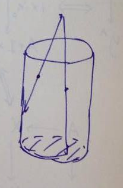
\includegraphics[scale=0.75]{retract-cofibration}
	\caption{Drawing by John Ni.}
    \end{figure}
    In particular, setting $n=1$ in this example, $\{0,1\}\hookrightarrow I$ is a cofibration.
\end{example}

The class of cofibrations is closed under the following operations.
\begin{itemize}
    \item Cobase change: if $A\to X$ is a cofibration and $A\to B$ is any map,
	the pushout $B\to X\cup_A B$ is again a cofibration.
    \item Coproducts.
    \item Composition.
\end{itemize}
Also, it satisfies the condition that we used to motivate the definition:
If $A\to X$ is a cofibration and $Y$ is an space, then $Y^X\to Y^A$ is a 
fibration. In particular, the map 
\[
ev_{0,1}:Y^I\to Y\times Y
\]
given by evaluation at the endpoints of the path is a fibration.

Finally, 
\begin{lemma} 
Any cofibration is a closed inclusion.
\end{lemma}

\begin{exercise}
An important (but easy!) fact about fibrations is that the canonical map 
$X\to \ast$ from any space $X$ is a fibration.
(Afficianados of model categories get excited about this 
because this says that all objects in the associated model structure on
topological spaces is fibrant.)
After all, this is a product projection! 
But the ``dual'' statement is false.    
Give an example of a compactly generated space $X$ containing a point
$*$ such that $\{*\}\hookrightarrow X$ is not a cofibration.
\end{exercise}
A basepoint $*$ is {\em nondegenerate} if $\{*\}\hookrightarrow X$ 
is a cofibration. 
If $\ast$ has a neighborhood in $X$ that contracts to $\{\ast\}$,
the inclusion $\ast\hookrightarrow X$ is a cofibration.
If $\ast$ is a nondegenerate basepoint of $A$, the evaluation map 
$\mathrm{ev}:X^A\to X$ is a fibration,
The fiber of $\mathrm{ev}$ over a basepoint of $X$ 
is exactly the space of pointed maps $X^A_*$.

\section{Homotopy fibers}

Fix a map $p:E\to Y$. The pullback of $E$ along a map $f:X\to Y$ can vary
wildly as $f$ is deformed; it is far from being a homotopy invariant. 
Just think of the case $X=*$, for example, when the pullback along 
$f:*\to Y$ is the point preimage $p^{-1}(f(*))$. One of the great
features of fibrations is this:

\begin{prop}
Let $p:E\to Y$ be a fibration and $f_0,f_1:X\to Y$ two maps.  
Write $E_0$ and $E_1$ for pullbacks of $E$ along $f_0$ and $f_1$.
If $f_0$ and $f_1$ are homotopic then $E_0$ and $E_1$ are homotopy
equivalent.
\end{prop}
\begin{proof}
Let $h:I\times X\to Y$ be a homotopy from $f_0$ to $f_1$. Its adjoint
is a path $\widehat h:I\to Y^X$ from $f_0$ to $f_1$. The fibration $p:E\to Y$
induces a fibration $E^X\to Y^X$, and the path determines a homotopy 
equivalence from the fiber over $f_0$ to the fiber over $f_1$. 
These two fibers are $E_0$ and $E_1$. 
\end{proof}

\subsection{``Fibrant replacements''}
This result makes fibrations extremely valuable in homotopy theory. 
Not every map is a fibration, but every map can be ``replaced'' by one, up
to homotopy.
\begin{theorem}\label{fibrep}
    For any map $f:X\to Y$, there is a space $T(f)$, along with a fibration $p:T(f) \to Y$ and
    a homotopy equivalence $X \xar{\simeq} T(f)$, such that the following diagram
    commutes:
    \begin{equation*}
	\xymatrix{
	    X\ar[r]^{\simeq}\ar[dr]_f & T(f)\ar[d]^p\\
	    & Y.
	    }
    \end{equation*}
\end{theorem}
\begin{proof}
We already have one example of this in hand: The diagonal map 
$\Delta:X\to X\times X$ factors as 
    \begin{equation*}
	\xymatrix{
	    X\ar[r]^{c}\ar[dr]_\Delta & X^I\ar[d]^{\mathrm{ev}_{0,1}}\\
	    & X\times X\,.
	    }
    \end{equation*}
where $p$ evaluates at the end points of the unit interval and $c$ sends
$x$ to the constant path at $x$. We've seen that $\mathrm{ev}_{0,1}$ 
is a fibration.
The map $c$ has as homotopy inverse any evaluation map, say $\mathrm{ev}_0$.
The composite $\mathrm{ev}_0\circ c$ is the identity, while 
$c\circ\mathrm{ev}_0$ is homotopic to the identity via the homotopy $h$ with
\[
h(s,\omega)(t)=\omega(st)\,.
\]
This ``spaghette move'' shortens the path from $\omega$ at $s=1$ to the 
constant path $c_{\omega(0)}$ at $s=0$. 

Now we can construct the general case by considering the graph of $f$ instead 
of the diagonal (which is the graph of the identity map). So form the pullback
	\begin{equation*}
	    \xymatrix{
T(f)\ar[r]\ar[d] \ar@/_3pc/[dd]_p & Y^I\ar[d]^{\mathrm{ev}_{0,1}}\\
		    X\times Y\ar[r]^{f\times 1} \ar[d]^{\pr_2} & Y\times Y\\
Y & 
		}
	\end{equation*}
so that
\[
T(f)=\{(x,\omega)\in X\times Y^I:f(x) = \omega(0)\}\,.
\]
The map $T(f)\to X\times Y$ 
is a base-change of the fibration $\mathrm{ev}_{0,1}$ and so is
a fibration; the projection map $\pr_2:X\times Y\to Y$ is a fibration; so
their composite $p$ is a fibration. To get $X$ involved, look at the diagram
\[
\xymatrix{
X \ar[r]^f \ar[d]^\Delta \ar@{.>}[dr] & Y \ar[dr]^c \\
X\times X \ar[dr]^{1\times f} & T(f) \ar[r] \ar[d] & 
Y^I \ar[d]^{\mathrm{ev}_{01}} \\
& X\times Y \ar[r]^{f\times1} \ar[d]^{\pr_1} & Y\times Y\\
& X && \,.
}\]
The outside diagram commutes, so we get a map from $X$ to the pullback $T(f)$. 
In symbols,
\[
x\mapsto(x,c_{f(x)})\,.
\]
We claim that the composite  $T(f)\to X\times Y\to X$ is a homotopy inverse. 
The composite $X\to T(f)\to X\times Y\to X$ is the identity, so we just need
a homotopy joining the other composite to the identity. Such a homotopy
$I\times T(f)\to T(f)$ is provided by the same spaghetti move: 
\[
(s,x,\omega)\mapsto(x,t\mapsto\omega(st))\,.
\]
\end{proof}

\begin{example}[Path-loop fibration]
        If $X = \ast$, the space $T(f)$ consists of paths $\omega$ in $Y$ such that $\omega(0) = \ast$.
    In other words, $T(f) = Y^I_\ast$; this is called the \emph{path space} of $Y$, and is denoted by $P(Y,\ast)$, or simply by $PY$. It is
contractible, via the spaghetti move. 
    The fiber over $\ast$ of the fibration $p:T(f) = PY \to Y$ consists of paths that begin and end at $\ast$, i.e., 
    loops on $Y$ based at $\ast$.
    This is denoted $\Omega Y$, and is called the \emph{loop space} of $Y$.
    The fibration $p:PY \to Y$ is called the \emph{path-loop fibration}.
\end{example}

\begin{exercise}[``Cofibrant replacements'']\label{cofibrep}
    In this exercise, you will prove the analogue of Theorem \ref{fibrep} for cofibrations.
    Let $f:X\to Y$ be any map.
    Show that $f$ factors (functorially) as a composite $X \to M \to Y$, where $X\to M$ is a cofibration and $M\to Y$ is a homotopy
    equivalence.
\end{exercise}

\subsection{Homotopy fibers}
Let $f:E\to Y$ a map. As you move around $Y$, the point preimages
generally vary, even up to homotopy type. They may become empty,
for example. We saw above that assuming that $f$ is a fibration
cures this problem,
and we have just seen that any map can be replaced, up to homotopy,
by a fibration. So it is sensible to make the following definition:
\begin{definition}
Let $(Y,*)$ be a pointed space. 
The \emph{homotopy fiber} of a map $f:E\to Y$ is the fiber over $*$ of
the fibration replacing $f$; that is, it is the pullback in
    \begin{equation*}
	\xymatrix{
	    F(f,\ast)\ar[r]\ar[d] & T(f)\ar[r]^\simeq \ar[d]^p & X\ar[dl]^f\\
	    \ast \ar[r] & Y & \,.
	    }
    \end{equation*}
\end{definition}
Homotopy fibers over different points in the same path component are homotopy
equivalent. 

As a set, 
\begin{equation}
\label{sethomotopyfiber}
F(f,\ast) = \{(x,\omega)\in E\times Y^I: \omega(0)=f(x), \omega(1) = \ast\}.
\end{equation}
So an element in the homotopy fiber of $f$ over $*$ is not just a
point in $E$ lying over $*\in Y$; it is a point $x\in E$ together with a path 
in $Y$ joining $f(x)$ to $\ast$ in $Y$. 

The inclusion of the fiber over $*\in Y$, $f^{-1}(*)\hookrightarrow E$,
is univeral among maps $g:W\to E$ such that $fg=*$. What is the corresponding
universal property of the homotopy fiber? Adjointing a map $W\to T(f)$ 
gives us a map $g:W\to E$ together with a homotopy from $fg$ to the constant 
map with value $*$: a {\em null homotopy} of the composite. 

\begin{remark} In forming the homotopy fiber of $f$, we replaced $f$ by
a homotopy equivalent fibration and formed the pullback over $*$. 
We could alternatively have replaced the map $*\to Y$ by a fibration
(the path-loop fibration!) and formed the pullback along $f$. The result of
this operation is
\[
\{(x,\omega)\in X\times Y^I:\omega(0) = \ast, \omega(1) = f(x)\}\,.
\]

Our description of $F(f,\ast)$ in \eqref{sethomotopyfiber} is almost exactly the same --- except that
the directions of the paths are reversed. These two ways of thinking of the
homotopy fiber are completely equivalent.
\end{remark}

\section{Barratt-Puppe sequence}\label{secbarrattpuppe}
%Hood's office hours are from 12 to 1:30 on Mondays in 2-390. Mine are from 4-5 on Tuesday in 2-478. Hood's graded the homework already.
\subsection{Fiber sequences}
Recall, from the previous section, that we have a pullback diagram:
\begin{equation*}
    \xymatrix{
	& F(f,\ast)\ar[r]\ar[d]^p \pb & PY\ar[d]^p\ar[dr]^{\simeq} & \\
	f^{-1}(\ast)\ar[ur]\ar[r] & X\ar[r]_f & Y & \ast\ar[l]
    }
\end{equation*}
Consider a pointed map\footnote{Some people call such a map ``based'', but this makes it sound like we're doing chemistry, so we won't use it.}
$f:X\to Y$ (so that $f(\ast) = \ast$). Then, we will write $Ff$ for the homotopy fiber $F(f,\ast)$.

Since we're exploring the homotopy fiber $Ff$, we can ask the following, seemingly silly, question:
what is the fiber of the canonical map $p:Ff\to X$ (over the basepoint of $X$)?
This is precisely the space of loops in $Y$!
Since $p$ is a fibration (recall that fibrations are closed under pullbacks), the homotopy fiber of $p$ is also the ``strict''
fiber!
Our expanded diagram is now:
\begin{equation*}
\xymatrix{\\
    & \Omega Y=p^{-1}(\ast)\ar[d] & & &\\
    & F(f,\ast)\ar[r]\ar[d]^p & PY\ar[d]^p\ar[dr]^{\simeq} & \\
    f^{-1}(\ast)\ar[ur]\ar[r] & X\ar[r]_f & Y & \ast.\ar[l]
}
\end{equation*}
It's easy to see that the composite $Ff\xar{p} X\xar{f} Y$ sends $(x,\omega)\mapsto f(x)$;
this is a pointed nonconstant map.
(Note that the basepoint we're choosing for $Ff$ is the image of the basepoint in $f^{-1}(\ast)$ under
the canonical map $f^{-1}(\ast)\hookrightarrow Ff$.)

While the composite $fp:Ff \to Y$ is not zero ``on the nose'', it is nullhomotopic, for instance
via the homotopy $h:Ff\times I\to Y$, defined by
$$h(t,(x,\omega)) = \omega(t).$$
\begin{exercise}\label{fiberkernel}
    Let $f:X\to Y$ and $g:W\to X$ be pointed maps.
    Establish a homeomorphism between the space of pointed maps $W \xar{p} Ff$ such that $fp = g$ and the space of pointed
    nullhomotopies of the composite $fg$.
\end{exercise}
This exercise proves that the homotopy fiber is the ``kernel'' in the homotopy category of pointed spaces and pointed
maps between them.

Define $[W,X]_\ast = \pi_0(X^W_\ast)$; this consists of the pointed homotopy classes of maps $W\to X$.
We may view this as a pointed set, whose basepoint is the constant map.
Fixing $W$, this is a contravariant functor in $X$, so there are maps $[W,Ff]_\ast\to [W,X]_\ast\to [W,Y]_\ast$.
This composite is not just nullhomotopic: it is ``exact''!
Since we are working with pointed sets, we need to describe what exactness means in this context:
the preimage of the basepoint in $[W,Y]_\ast$ is exactly the image of $[W,Ff]_\ast\to [W,X]_\ast$.
(This is exactly a reformulation of Exercise \ref{fiberkernel}.)
We say that $Ff\to X\xrightarrow{f}Y$ is a \emph{fiber sequence}.

\begin{remark}
    Let $f:X\to Y$ be a map of spaces, and suppose we have a homotopy commutative diagram:
    \begin{equation*}
	\xymatrix{
	    \Omega Y\ar[d]_{\Omega g}\ar[r] & Ff\ar@{-->}[d]\ar[r] & X\ar[d]_{h}\ar[r]^f & Y\ar[d]^g\\
	    \Omega Y^\prime\ar[r] & Ff^\prime\ar[r] & X^\prime\ar[r]_{f^\prime} & Y.
	    }
    \end{equation*}
    Then the dotted map exists, but it {depends on the homotopy} $f^\prime h\simeq gf$. 
\end{remark}

\subsection{Iterating fiber sequences}
Let $f:X\to Y$ be a pointed map, as before.
As observed above, we have a composite map $Ff\xrightarrow{p} X\xrightarrow{f} Y$, and
the strict fiber (homotopy equivalent to the homotopy fiber) of $p$ is $\Omega Y$.
This begets a map $i(f):\Omega Y\to Ff$; iterating the procedure of taking fibers gives:
\begin{equation*}
    \xymatrix{
	\cdots\ar[r] & Fp_3 \ar[r]^{p_4} & Fp_2\ar[r]^{p_3} & Fp_1\ar[r]^{p_2} & Ff\ar[r]^{p_1} & X\ar[r]^{f} & Y\\
	& \Omega Fp_0\ar[u]|{\simeq}\ar[ur]|{i(p_2)}\ar@{-->}[r] & \Omega X\ar@{-->}[r]\ar[u]|{\simeq}\ar[ur]|{i(p_1)} & \Omega Y\ar[u]|\simeq \ar[ur]|{i(f)} & &
    }
\end{equation*}
All the $p_i$ in the above diagram are fibrations.
Each of the dotted maps in the above diagram can be filled in up to homotopy.
The most obvious guess for what these dotted maps are is simply $\Omega X\xrightarrow{\Omega f}\Omega Y$.
But \emph{that is the wrong map}!

The right map turns out to be $\Omega X\xrightarrow{\overline{\Omega f}}\Omega Y$:
\begin{lemma}
    The following diagram commutes to homotopy:
    \begin{equation*}
	\xymatrix{
	    & Fp\\
	    \Omega X\ar[r]_{\overline{\Omega f}}\ar[ur]^{i(p)} & \Omega Y;\ar[u]
	    }
    \end{equation*}
    here, $\overline{\Omega f}$ is the diagonal in the following diagram:
    \begin{equation*}
	\xymatrix{
	    \Omega X\ar[r]^{-}\ar[dr]|{\Omega f} \ar[d]_{\Omega f} & \Omega X\ar[d]^{\Omega f}\\
	    \Omega Y\ar[r]_{-} & \Omega Y,
	    }
    \end{equation*}
    where the map $-:\Omega X\to \Omega X$ sends $\omega\mapsto\overline{\omega}$.
\end{lemma}
\begin{proof}
    \todo{typeset the following image for the proof... it's going to be impossible to write this up in symbols.}
\begin{figure}[H]
\centering
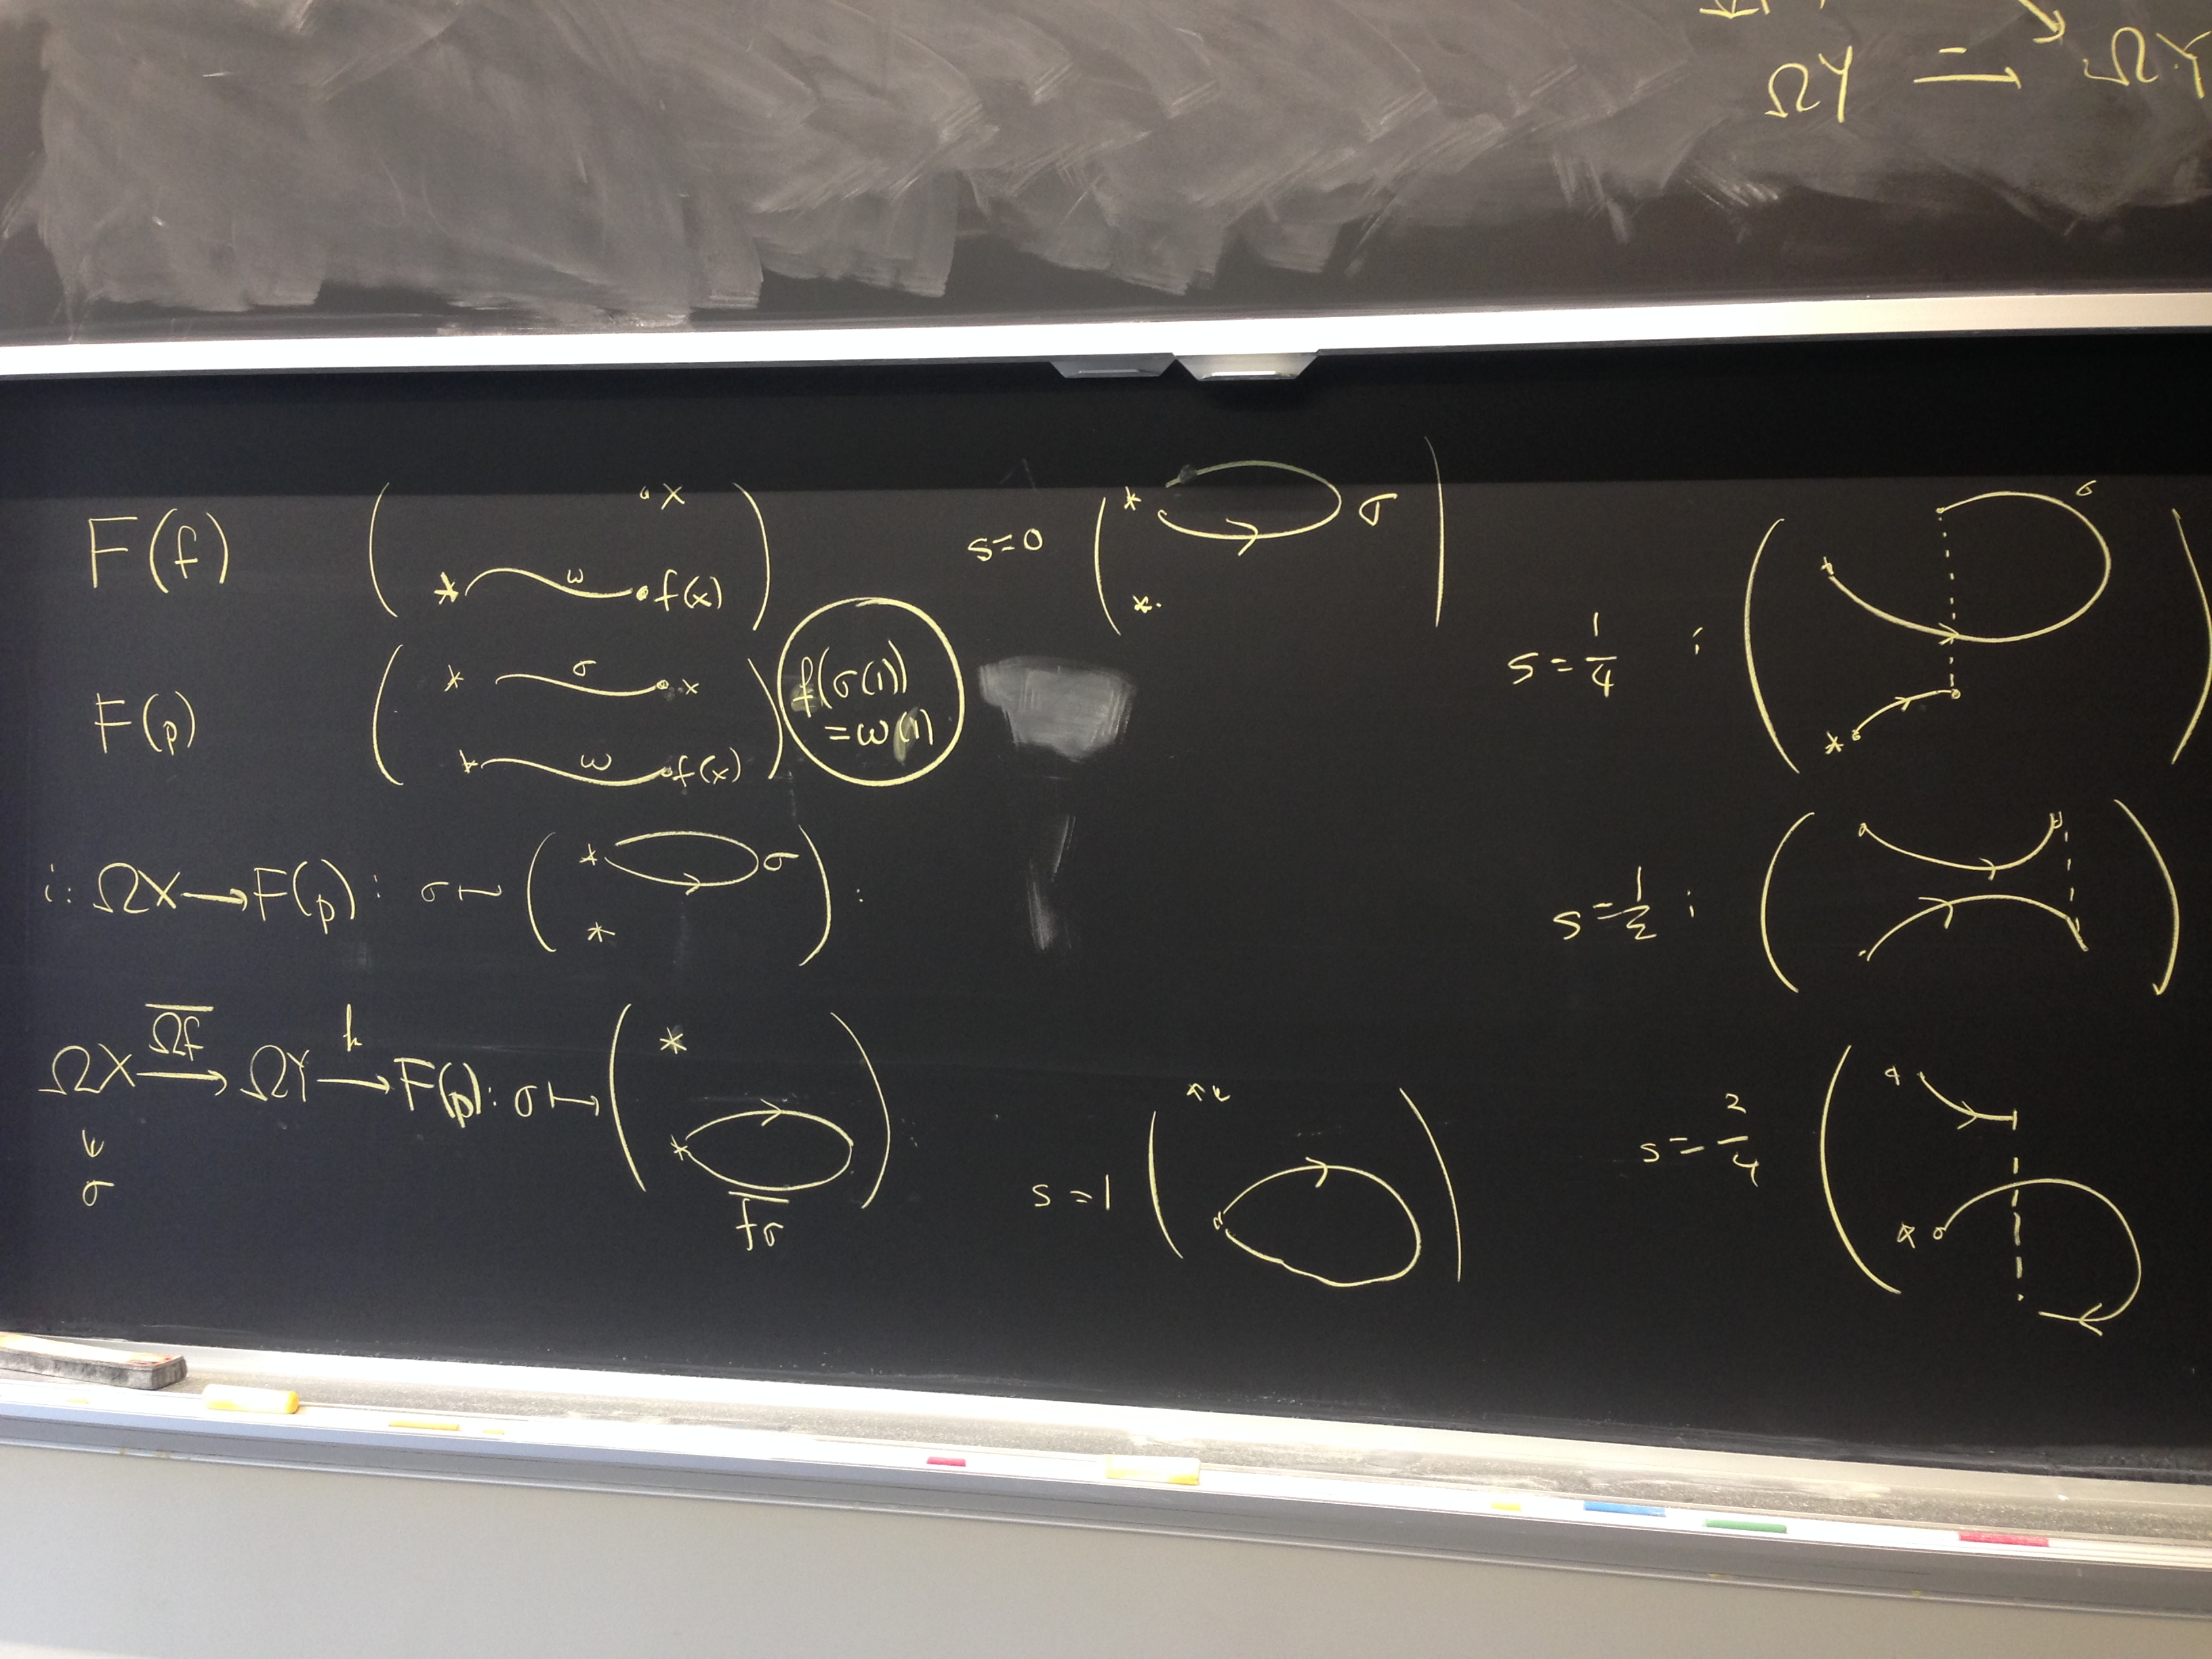
\includegraphics[width=\textwidth]{barratt-puppe}
\caption{A proof of this lemma.}
\end{figure}
\end{proof}
%\begin{lemma}
%    The following diagram commutes:
%    \begin{equation*}
%	\xymatrix{
%	    & F(\overline{\Omega p_0})\ar@{=}[dd]\ar[dr] & \\
%	    \Omega^2 Y\ar[ur]^{i(\Omega p_0)}\ar[dr]_{\overline{\Omega i(p_0)}} & & \Omega X\\
%	    & \Omega Fp_0\ar[ur]_{\overline{\Omega p_1}} & 
%	    }
%    \end{equation*}
%\end{lemma}
%What is the map $F\overline{\Omega p_0}\to \Omega X$?? We spent some time figuring this out.
%But you can now apply $[W,-]_\ast$ to the following diagram to get a long exact sequence:
By the above lemma, we can extend our diagram to:
\begin{equation*}
    \xymatrix{
	\cdots\ar[r] & Fp_4\ar[r] & Fp_3 \ar[r] & Fp_2\ar[r] & Fp_1\ar[r]^{p_2} & Ff\ar[r]^{p_1} & X\ar[r]^{f} & Y\\
    \cdots\ar[r] & \Omega Fp_1\ar[r]|{\overline{\Omega p_2}}\ar[u]_{\simeq} & \Omega Ff\ar[u]_{\simeq}\ar[ur]|{i(p_2)}\ar[r]|{\overline{\Omega p}} & \Omega X\ar[r]|{\overline{\Omega f}}\ar[u]_{\simeq}\ar[ur]|{i(p_1)} & \Omega Y\ar[u]_\simeq \ar[ur]|{i(f)} & &\\
	\Omega^2 X\ar[u]_{\simeq}\ar[r]_{\Omega^2 f} & \Omega^2 Y\ar[u]_{\simeq}\ar[ur]_{\overline{\Omega i(p_0)}} & & &
    }
\end{equation*}
We have a special name for the sequence of spaces sneaking along the bottom of this diagram:
$$\cdots\to \Omega^2 X \to \Omega^2 Y \to \Omega Ff \to \Omega X \to \Omega Y \to Ff \to X \xar{f} Y;$$
this is called the \emph{Barratt-Puppe sequence}.
Applying $[W,-]_\ast$ to the Barratt-Puppe sequence of a map $f:X\to Y$ gives a long exact sequence.

The most important case of this long exact sequence comes from setting $W = S^0=\{\pm 1\}$;
in this case, we get terms like $\pi_0(\Omega^n X)$.
We can identify $\pi_0(\Omega^n X)$ with $[S^n,X]_\ast$: to see this for $n=2$,
recall that $\Omega^2 X = (\Omega X)^{S^1}$; because $(S^1)^{\wedge n} = S^n$ (see below for a proof of this fact), 
we find that
\begin{equation}\label{bpsequence}
(\Omega X)^{S^1} \simeq (X^{S^1}_\ast)^{S^1}_\ast = X_\ast^{S^1\wedge S^1} = X_\ast^{S^2},
\end{equation}
as desired.

The space $\Omega X$ is a group in the homotopy category; this implies that
$\pi_0 \Omega X = \pi_1 X$ is a group!
For $n>1$, we know that
$$\pi_n(X) = [(D^n,S^{n-1}),(X,\ast)] = [(I^n,\partial I^n),(X,\ast)].$$
\begin{exercise}
    Prove that $\pi_n(X)$ is an abelian group for $n>2$.
\end{exercise}
%Suppose $n=2$, for simplicity.
%How do I take the product of $\alpha,\beta\in \pi_2(X)$?
%Thinking of $\pi_2(X)$ as $[(I^2,\partial I^2),(X,\ast)]$ tells us that . You can play this game; up to homotopy, you can shrink $\alpha$ and $\beta$ to make them as small I want, and then reverse their position and expand them again\footnote{This probably makes no sense without a picture}\todo{Add a picture}. Thus $\pi_2(X)$ is an abelian group.
Applying $\pi_0$ to the Barratt-Puppe sequence (see Equation \ref{bpsequence}) therefore gives a long exact sequence
(of groups when the homotopy groups are in degrees greater than $0$, and of pointed sets in degree $0$):
$$\cdots\to \pi_2 X\to \pi_2 Y\to \pi_1 Ff\to \pi_1 X\to\pi_1 Y\to\pi_0 Ff\to\pi_0 X\to \pi_0 X.$$

\section{Relative homotopy groups}
%Pset 2 has question 8; there's still one more to go. Hood has office hours today 12 -- 1 in 2-390, and I have office hours today tomorrow 4-5 in 2-478.
\subsection{Spheres and homotopy groups}
The functor $\Omega$ (sending a space to its based loop space) admits a left adjoint.
To see this, recall that $\Omega X = X^{S^1}_\ast$, so that
$$\Top_\ast(W,\Omega X) = \Top_\ast(S^1\wedge W,X).$$
\begin{definition}
    The \emph{reduced suspension} $\Sigma W$ is $S^1\wedge W$.
\end{definition}
If $A\subseteq X$, then
$$X/A\wedge Y/B = (X\times Y)/((A\times Y)\cup_{A\times B}(X\times B)).$$
Since $S^1 = I/\partial I$, this tells us that $\Sigma X = S^1\wedge X$ can be identified with
$I\times X/(\partial I \times X\cup I\times \ast)$: in other words, we collapse the top and bottom of a cylinder to a point,
as well as the line along a basepoint.

The same argument says that $\Sigma^n X$ (defined inductively as $\Sigma(\Sigma^{n-1} X)$)
is the left adjoint of the $n$-fold loop space functor $X\mapsto \Omega^n X$.
In other words, $\Sigma^n X = (S^1)^{\wedge n}\wedge X$.
We claim that $S^1\wedge S^n \simeq S^{n+1}$.
To see this, note that
$$S^1\wedge S^n = I/\partial I\wedge I^n\wedge \partial I^n = (I\times I^n)/(\partial I\times I^n\cup I\times \partial I^n).$$
The denominator is exactly $\partial I^{n+1}$, so $S^1\wedge S^n\simeq S^{n+k}$.
It's now easy to see that $S^k\wedge S^n\simeq S^{k+n}$.
\begin{definition}
    The \emph{$n$th homotopy group} of $X$ is $\pi_n X = \pi_0(\Omega^n X)$.
\end{definition}
This is, as we noted in the previous section, $[S^0,\Omega^n X]_\ast = [S^n, X]_\ast = [(I^n,\partial I^n),(X,\ast)]$.

\subsection{The homotopy category}
Define the \emph{homotopy category of spaces} $\Ho(\Top)$ to be the category
whose objects are spaces, and whose hom-sets are given by taking $\pi_0$ of the mapping space.
To check that this is indeed a category, we need to check that if $f_0,f_1:X\to Y$ and $g:Y\to Z$, then $gf_0\simeq gf_1$ ---
but this is clear.
Similarly, we'd need to check that $f_0h\simeq f_1h$ for any $h:W\to X$.
We can also think about the homotopy category of pointed spaces (and pointed homotopies) $\Ho(\Top_\ast)$; this is the category
we have been spending most of our time in.
Both $\Ho(\Top)$ and $\Ho(\Top_\ast)$ have products and coproducts, but very few other limits or colimits.
From a category-theoretic standpoint, these are absolutely terrible.

Let $W$ be a pointed space.
We would like the assignment $X\mapsto X^W_\ast$ to be a homotopy functor.
It clearly defines a functor $\Top_\ast\to\Top_\ast$, so this desire is equivalent to providing a dotted arrow in the
following diagram:
\begin{equation*}
    \xymatrix{
	\Top_\ast\ar[d]\ar[r]^{X\mapsto X^W_\ast} & \Top_\ast\ar[d]\\
	\Ho(\Top_\ast)\ar@{-->}[r] & \Ho(\Top_\ast).
    }
\end{equation*}
Before we can prove this, we will check that a homotopy $f_0\sim f_1:X\to Y$ is the same as a map $I_+\wedge X\to Y$.
There is a nullhomotopy if the basepoint of $I$ is one of the endpoints, so a homotopy is the same as a map
$I\times X/I\times\ast \to Y$. The source is just $I_+\wedge X$, as desired.

A homotopy $f_0 \simeq f_1:X\to Y$ begets a map $(I_+\wedge X)^W\to Y^W_\ast$.
For the assignment $X\mapsto X^W_\ast$ to be a homotopy functor, we need a natural transformation $I_+\wedge X^W_\ast\to Y^W_\ast$, so this map is not quite what's necessary.
Instead, we can attempt to construct a map $I_+\wedge X^W_\ast\to (I_+\wedge X)^W_\ast$.

We can construct a general map $A\wedge X^W_\ast\to (A\wedge X)^W_\ast$: 
there is a map $A\wedge X^W_\ast\to A^W_\ast\wedge X^W_\ast$, given by sending $a\mapsto c_a$;
then the exponential law gives a homotopy $A^W_\ast\wedge X^W_\ast\to (A\wedge X)^W_\ast$.
This, in turn, gives a map $I_+\wedge X^W_\ast\to (I_+\wedge X)^W_\ast\to Y^W_\ast$,
thus making $X\mapsto X^W_\ast$ a homotopy functor.

Motivated by our discussion of homotopy fibers, we can study composites which ``behave'' like short exact sequences.
\begin{definition}
    A \emph{fiber sequence} in $\Ho(\Top_\ast)$ is a composite $X\to Y\to Z$ that is
    isomorphic, in $\Ho(\Top_\ast)$, to some composite $Ff\xrightarrow{p} E\xrightarrow{f}B$;
    in other words, there exist (possibly zig-zags of) maps that are homotopy equivalences, that make the following
    diagram commute:
    \begin{equation*}
	\xymatrix{
	    X\ar[r]\ar[d] & Y\ar[r]\ar[d] & Z\ar[d]\\
	    Ff\ar[r]_p & E\ar[r]_f & B.
	    }
    \end{equation*}
\end{definition}
Let us remark here that if $A^\prime \xar{\sim} A$ is a homotopy equivalence, and $A\to B \to C$ is a fiber sequence, so
is the composite $A^\prime\xar{\sim} A \to B\to C$.

\begin{exercise}\label{loopslimit}
    Prove the following statements.
    \begin{itemize}
	\item $\Omega$ takes fiber sequences to fiber sequences.
	\item $\Omega Ff\simeq F\Omega f$. Check this!
    \end{itemize}
\end{exercise}

We've seen examples of fiber sequences in our elaborate study of the Barratt-Puppe sequence.
\begin{example}
Recall our diagram:
\begin{equation*}
    \xymatrix{
	\cdots\ar[r] & Fp_4\ar[r] & Fp_3 \ar[r] & Fp_2\ar[r] & Fp_1\ar[r]^{p_2} & Ff\ar[r]^{p_1} & X\ar[r]^{f} & Y\\
    \cdots\ar[r] & \Omega Fp_1\ar[r]|{\overline{\Omega p_2}}\ar[u]_{\simeq} & \Omega Ff\ar[u]_{\simeq}\ar[ur]|{i(p_2)}\ar[r]|{\overline{\Omega p}} & \Omega X\ar[r]|{\overline{\Omega f}}\ar[u]_{\simeq}\ar[ur]|{i(p_1)} & \Omega Y\ar[u]_\simeq \ar[ur]|{i(f)} & &\\
	\Omega^2 X\ar[u]_{\simeq}\ar[r]_{\Omega f} & \Omega Y\ar[u]_{\simeq}\ar[ur]_{\overline{\Omega i(f)}} & & &
    }
\end{equation*}
The composite $Ff\to X\xar{f} Y$ is canonically a fiber sequence.
The above diagram shows that $\Omega Y\to F\xrightarrow{p}X$ is another fiber sequence: it is isomorphic to
$Fp\to F\to X$ in $\Ho(\Top_\ast)$.
Similarly, the composite $\Omega X\xrightarrow{\overline{\Omega f}}\Omega Y\to F$ is another fiber sequence;
this implies that $\Omega X\xrightarrow{\Omega f}\Omega Y\to F$ is also an example of a fiber sequence
(because these two fiber sequences differ by an automorphism of $\Omega X$)

Applying $\Omega$ again, we get $\Omega F\xrightarrow{\Omega p} \Omega X\xrightarrow{\Omega f} \Omega Y$.
Since this is a looping of a fiber sequence, and taking loops takes fiber sequences to fiber sequences (Exercise \ref{loopslimit}), this is another fiber sequence. 
Looping again gives another fiber sequence $\Omega^2 Y\xrightarrow{\Omega i} \Omega F\xrightarrow{\Omega p}\Omega X$.
(For the category-theoretically--minded folks, this is an unstable version of a triangulated category.)
\end{example}

\subsection{The long exact sequence of a fiber sequence}
As discussed at the end of \S \ref{secbarrattpuppe}, applying $\pi_0 = [S^0,-]_\ast$ to the
Barratt-Puppe sequence associated to a map $f:X\to Y$ gives a long exact sequence:
\begin{equation*}
    \xymatrix{
	& \cdots\ar[r] & \pi_2 Y\ar[dll]\\
	\pi_1 F\ar[r] & \pi_1 X\ar[r] & \pi_1 Y\ar[dll]\\
	\pi_0 F\ar[r] & \pi_0 X. & 
    }
\end{equation*}
of pointed sets.
The space $\Omega^2 X$ is an \emph{abelian} group object in $\Ho(\Top)$
(in other words, the multiplication on $\Omega^2 X$ is commutative up to homotopy).
This implies $\pi_1(X)$ is a group, and that $\pi_k(X)$ is abelian for $k\geq 2$;
hence, in our diagram above, all maps (except on $\pi_0$) are group homomorphisms.

Consider the case when $X\to Y$ is the inclusion $i:A\hookrightarrow X$ of a subspace.
In this case,
$$Fi=\{(a,\omega)\in A\times X^I_\ast|\omega(1) = a\};$$
this is just the collection of all paths that begin at $\ast\in A$ and end in $A$.
This motivates the definition of \emph{relative homotopy groups}:
\begin{definition}
    Define: 
    $$\pi_n(X,A,\ast) = \pi_n(X,A) := \pi_{n-1}Fi = [(I^n,\partial I^n,(\partial I^n\times I)\cup (I^{n-1}\times 0)),(X,A,\ast)].$$
\end{definition}
We have a sequence of inclusions
$$\partial I^n\times I\cup I^{n-1}\times 0 \subset \partial I^n \subset I^n.$$
One can check that
$$\pi_{n-1}Fi = [(I^n,\partial I^n,(\partial I^n\times I)\cup (I^{n-1}\times 0)),(X,A,\ast)].$$
This gives a long exact sequence on homotopy, analogous to the long exact sequence in relative homology:
\begin{equation}\label{lexseqhomotopy}
    \xymatrix{
	& \cdots\ar[r] & \pi_2 (X,A)\ar[dll]\\
	\pi_1 A\ar[r] & \pi_1 X\ar[r] & \pi_1 (X,A)\ar[dll]\\
	\pi_0 A\ar[r] & \pi_0 X & 
    }
\end{equation}

\section{Action of $\pi_1$, simple spaces, and the Hurewicz theorem}
In the previous section, we constructed a long exact sequence of homotopy groups:
\begin{equation*}
    \xymatrix{
	& \cdots\ar[r] & \pi_2 (X,A)\ar[dll]\\
	\pi_1 A\ar[r] & \pi_1 X\ar[r] & \pi_1 (X,A)\ar[dll]\\
	\pi_0 A\ar[r] & \pi_0 X, & 
    }
\end{equation*}
which looks suspiciously similar to the long exact sequence in homology.
The goal of this section is to describe a relationship between homotopy groups and homology groups.

Before we proceed, we will need the following lemma.
\begin{lemma}[Excision]
    If $A\subseteq X$ is a cofibration, there is an isomorphism
    $$H_\ast(X,A)\xrightarrow{\simeq}\widetilde{H}_\ast(X/A).$$
    Under this hypothesis,
    $$X/A\simeq\text{Mapping cone of }i:A\to X;$$
    here, the mapping cone is the homotopy pushout in the following diagram:
    \begin{equation*}
	\xymatrix{
	    A\ar[r]^i\ar[d]^{in_1} & X\ar[d]\\
	    CA\ar[r] & X\cup_A CA,
	    }
    \end{equation*}
    where $CA$ is the cone on $A$, defined by
    $$CA = A\times I/A\times 0.$$
\end{lemma}
This lemma is dual to the statement that the homotopy fiber is homotopy equivalent to the strict fiber for fibrations.

Unfortunately, $\pi_\ast(X,A)$ is definitely not $\pi_\ast(X/A)$!
For instance, there is a cofibration sequence
$$S^1\to D^2\to S^2.$$
We know that $\pi_\ast S^1$ is just $\Z$ in dimension $1$, and is zero in other dimensions.
On the other hand, we do not, and probably will never, know the homotopy groups of $S^2$.
(A theorem of Edgar Brown in \cite{brown-computability} says that these groups are computable, but this is super-exponential.)
%\begin{theorem}[Now]
%    If $X$ is a simply connected finite complex, and $X\not\simeq \ast$, then we do not know $\pi_\ast(X)$. And we'll probably never be able to know them.
%\end{theorem}
%These groups \emph{are} computable (a theorem by Edgar Brown), but it's super-exponential. This is discouraging. We'll never know what, eg., $\pi_{10000}(S^2)$ is.

%Anyway, I said there was $\partial:\pi_n(X,A,\ast)\to \pi_{n-1}(A,\ast)$. How does this look? Well you just look at the restriction of $I^n\to X$ to $1\times I^{n-1}\to A$. And the composite $\pi_n(X,A,\ast)\xrightarrow{\partial}\pi_{n-1}(A,\ast)\to \pi_{n-1}(X,\ast)$ is trivial by definition!
\subsection{$\pi_1$-action}
There is more structure in the long exact sequence in homotopy groups that we constructed last time, coming from an action
of $\pi_1(X)$.
There is an action of $\pi_1(X)$ on $\pi_n(X)$: if $x,y$ are points in $X$, and $\omega:I\to X$ is a path with $\omega(0) = x$ and $\omega(1) = y$, we have a map $f_\omega:\pi_n(X,x)\to \pi_n(X,y)$;
this, in particular, implies that $\pi_1(X,\ast)$ acts on $\pi_n(X,\ast)$.
When $n=1$, the action $\pi_1(X)$ on itself is by conjugation.

In fact, one can also see that $\pi_1(A)$ acts on $\pi_n(X,A,\ast)$.
It follows (by construction) that all maps in the long exact sequence of Equation \eqref{lexseqhomotopy} are equivariant for
this action of $\pi_1(A)$.
Moreover:
\begin{prop}[Peiffer identity]
    Let $\alpha,\beta\in \pi_2(X,A)$. Then $(\partial \alpha)\cdot\beta = \alpha\beta\alpha^{-1}$.
\end{prop}
%For example, if $j:\pi_2(X)\to \pi_2(X,A)$, and $\alpha = j(\gamma)$, $\partial\alpha = 1$: $\img(k)\subseteq\coker \pi_2(X,A)$. (I did not follow this)

\begin{definition}
    A topological space $X$ is said to be \emph{simply connected} if it is path connected, and $\pi_1(X,\ast) = 1$.
\end{definition}
Let $p:E\to B$ be a covering space with $E$ and $B$ connected.
Then, the fibers are discrete, hence do not have any higher homotopy.
Using the long exact sequence in homotopy groups, we learn that $\pi_n(E)\to \pi_n(B)$ is an isomorphism for $n>1$,
and that $\pi_1(E)$ is a subgroup of $\pi_1(B)$ that classifies the covering space.
In general, we know from Exercise \ref{simplequotient} that $\Omega B$ acts on the homotopy fiber $Fp$.
Since $Ff$ is discrete, this action factors through $\pi_0(\Omega B)\simeq \pi_1(B)$.

%In particular, $\pi_q(S^n)\simeq \pi_q(\RP^n)$ for $q>1$. Of course, $\pi_1(\RP^n)\simeq \Z/2\Z$. This creates a ton of homology in $\RP^n$ that's not present in the homology of $S^n$. Here's a piece of language.
\begin{definition}
    A space $X$ is said to be \emph{$n$-connected} if $\pi_i(X) = 0$ for $i\leq n$.
\end{definition}
Note that this is a well-defined condition, although we did not specify the basepoint: $0$-connected implies path connected.
Suppose $E\to B$ is a covering space, with the total space $E$ being $n$-connected.
Then, Hopf showed that the group $\pi_1(B)$ determines the homology $H_i(B)$ in dimensions $i<n$.
%in particular, $H_i(B) = H_i(\pi_1(B))$, which is the group homology. This is due to Heinz Hopf.

Sometimes, there are interesting spaces which are not simply connected, for which the $\pi_1$-action is nontrivial.
\begin{example}
    Consider the space $S^1\vee S^2$.
    The universal cover is just $\RR$, with a $2$-sphere $S^2$ stuck on at every integer point.
    This space is simply connected, so the Hurewicz theorem says that $\pi_2(E)\simeq H_2(E)$.
    Since the real line is contractible, we can collapse it to a point: this gives a countable bouquet of $2$-spheres.
    As a consequence, $\pi_2(E)\simeq H_2(E) = \bigoplus_{i=0}^\infty \Z$.

    There is an action of $\pi_1(S^1\vee S^2)$ on $E$: the action does is shift the $2$-spheres on the integer points of $\RR$ (on $E$) to the right by $1$ (note that $\pi_1(S^1\vee S^2) = \Z$).
    This tells us that $\pi_2(E) \simeq \Z[\pi_1(B)]$ as a $\Z[\pi_1(B)]$-module; this is the same action of $\pi_1(E)$ on
    $\pi_2(E)$.
    We should be horrified: $S^1\vee S^2$ is a very simple $3$-complex, but its homotopy is huge!
\end{example}
Simply-connectedness can sometimes be a restrictive condition; instead, to simplify the long exact sequence, we define:
\begin{definition}
    A topological space $X$ is said to be \emph{simple} if it is path-connected, and
    $\pi_1(X)$ acts trivially on $\pi_n(X)$ for $n\geq 1$.
\end{definition}
Note, in particular, that $\pi_1(X)$ is abelian for a simple space.

Being simple is independent of the choice of basepoint. If $\omega:x\mapsto x^\prime$ is a path in $X$,
then $\omega_\sharp:\pi_n(X,x)\to \pi_n(X,x^\prime)$ is a group isomorphism.
There is a (trivial) action of $\pi_1(X,x)$ on $\pi_n(X,x)$, and another (potentially nontrivial)
action of $\pi_1(X,x^\prime)$ on $\pi_n(X,x^\prime)$.
Both actions are compatible: hence, if $\pi_1(X,x)$ acts trivially, so does $\pi_1(X,x^\prime)$.

If $X$ is path-connected, there is a map $\pi_n(X,\ast)\to [S^n,X]$.
It is clear that this map is surjective,
%because I can always choose a basepoint in $X$ as the image of a basepoint in $S^n$.
so one might expect a factorization:
\begin{equation*}
    \xymatrix{
	\pi_n(X,\ast)\ar@{->>}[r]\ar[dr] & [S^n,X]\\
	& \pi_1(X,\ast)\backslash \pi_n(X,\ast)\ar[u]
	}
\end{equation*}
\begin{exercise}\label{simplequotient}
    %Exercises 7 and 9 of pset 2
    Prove that $\pi_1(X,\ast)\backslash \pi_n(X,\ast) \simeq [S^n, X]$.
    To do this, work through the following exercises.
    
    Let $f:X\to Y$ be a map of spaces, and let $\ast\in Y$ be a fixed basepoint of $Y$.
    Denote by $Ff$ the homotopy fiber of $f$; this admits a natural fibration $p:Ff \to X$, given by $(x,\sigma)\mapsto x$.
    If $\Omega Y$ denotes the (based) loop space of $Y$, we get an action $\Omega Y \times Ff \to Ff$, given by
    $$(\omega,(x,\sigma)) \mapsto (x,\sigma\cdot\omega),$$
    where $\sigma\cdot\omega$ is the concatenation of $\sigma$ and $\omega$, defined, as usual, by
    $$
    \sigma\cdot\omega(t) = \begin{cases}
	\omega(2t) & 0\leq t\leq 1/2\\
	\sigma(2t-1) & 1/2\leq t\leq 1.
    \end{cases}
    $$
    (Note that when $X$ is the point, this defines a ``multiplication'' $\Omega Y \times \Omega Y \to \Omega Y$; this is 
    associative and unital up to homotopy.)
    On connected components, we therefore get an action of $\pi_0\Omega Y \simeq \pi_1 Y$ on $\pi_0 Ff$.

    There is a canonical map
    $$Ff \times \Omega Y \to Ff\times_X Ff,$$
    given by $((x,\sigma),\omega) \mapsto ((x,\sigma),(x,\sigma)\cdot\omega)$.
    Prove that this map is a homotopy equivalence (so that the action of $\Omega Y$ on $Ff$ is ``free''), and conclude that
    two elements in $\pi_0 Ff$ map to the same element of $\pi_0 X$ if and only if they are in the same orbit under the action
    of $\pi_1 Y$.

    Let $X$ be path connected, with basepoint $\ast\in X$.
    Conclude that $\pi_1(X,\ast)\backslash \pi_n(X,\ast) \simeq [S^n,X]$ by proving that the surjection
    $\pi_n(X,\ast) \to [S^n,X]$ can be identified with the orbit projection for the action of $\pi_1(X,\ast)$ on $\pi_n(X,\ast)$.
\end{exercise}
If $X$ is simple, then the quotient $\pi_1(X,\ast)\backslash \pi_n(X,\ast)$ is simply $\pi_n(X, \ast)$, so
Exercise \ref{simplequotient} implies that $\pi_n(X,\ast)\cong [S^n,X]$ --- independently of the basepoint;
in other words, these groups are canonically the same, i.e., two paths $\omega,\omega^\prime:x\to y$ give the
same map $\omega_\sharp = \omega^\prime_\sharp:\pi_n(X,x)\to \pi_n(X,y)$.

\begin{exercise}
    A \emph{$H$-space} is a pointed space $X$, along with a pointed map $\mu:X\times X \to X$, such that the maps
    $x\mapsto \mu(x,\ast)$ and $x\mapsto \mu(\ast,x)$ are both pointed homotopic to the identity.
    In this exercise, you will prove that path connected $H$-spaces are simple.
    
    Denote by $\cc$ the category of pairs $(G,H)$, where $G$ is a group that acts on the group $H$ (on the left); the morphisms
    in $\cc$ are pairs of homomorphisms which are compatible with the group actions.
    This category has finite products.
    Explain what it means for an object of $\cc$ to have a ``unital multiplication'', and prove that any object $(G,H)$ of $\cc$
    with a unital multiplication has $G$ and $H$ abelian, and that the $G$-action on $H$ is trivial.
    Conclude from this that path connected $H$-spaces are simple.
\end{exercise}
\subsection{Hurewicz theorem}
\begin{definition}
    Let $X$ be a path-connected space.
    The Hurewicz map $h:\pi_n(X,\ast)\to H_n(X)$is defined as follows:
    an element in $\pi_n(X,\ast)$ is represented by $\alpha:S^n\to X$; pick a generator $\sigma\in H_n(S^n)$, and send
    $$\alpha\mapsto\alpha_\ast(\sigma)\in H_n(X).$$
\end{definition}
We will see below that $h$ is in fact a homomorphism.

This is easy in dimension $0$: a point is a $0$-cycle!
In fact, we have an isomorphism $H_0(X)\simeq \Z[\pi_0(X)]$.
(This isomorphism is an example of the Hurewicz theorem.)

When $n=1$, we have $h:\pi_1(X,\ast)\to H_1(X)$. Since $H_1(X)$ is abelian, this factors as
$\pi_1(X,\ast)\to \pi_1(X,\ast)^{ab}\to H_1(X)$.
The Hurewicz theorem says that the map $\pi_1(X,\ast)^{ab}\to H_1(X)$ is an isomorphism.
We will not prove this here; see \cite[Theorem 2A.1]{hatcher} for a proof.

The Hurewicz theorem generalizes these results to higher dimensions:
\begin{theorem}[Hurewicz]
    Suppose $X$ is a space for which $\pi_i(X) = 0$ for $i<n$, where $n\geq 2$.
    Then the Hurewicz map $h:\pi_n(X)\to H_n(X)$ is an isomorphism.
\end{theorem}

Before the word ``isomorphism'' can make sense, we need to prove that $h$ is a homomorphism.
Let $\alpha,\beta:S^n\to X$ be pointed maps. The product $\alpha\beta\in \pi_n(X)$ is the composite:
$$\alpha\beta:S^n\xrightarrow{\delta\text{, pinching along the equator}} S^n\vee S^n\xrightarrow{\beta\vee\alpha}X\vee X\xrightarrow{\nabla}X,$$
where $\nabla:X\vee X\to X$ is the fold map, defined by:
\begin{equation*}
    \xymatrix{
	X\ar[dr]^1\ar[d] & \\
	X\vee X\ar[r]|\nabla & X\\
	X\ar[u]\ar[ur]_1 & 
    }
\end{equation*}
%We have two inclusions $\mathrm{in}_1,\mathrm{in}_2$ of $S^n$ to $S^n\vee S^n$.
%If $\sigma\in H_n(S^n)$ is a generator, the composite
%$$\sigma\mapsto {in_1}_\ast\sigma + {in_2}_\ast\sigma\mapsto {in_1}_\ast h(\alpha) + {in_2}_\ast h(\beta)\mapsto h(\alpha) + h(\beta)$$
%\todo{edit from here}
%As desired.
To show that $h$ is a homomorphism, it suffices to prove that for two maps $\alpha,\beta:S^n \to X$, the induced maps on homology
satisfy $(\alpha+\beta)_\ast = \alpha_\ast + \beta_\ast$ --- then,
$$h(\alpha+\beta) = (\alpha+\beta)_\ast(\sigma) = \alpha_\ast(\sigma) + \beta_\ast(\sigma) = h(\alpha) + h(\beta).$$
To prove this, we will use the pinch map $\delta:S^n \to S^n \vee S^n$, and the quotient maps $q_1,q_2:S^n\vee S^n \to S^n$;
the induced map $H_n(S^n) \to H_n(S^n) \oplus H_n(S^n)$ is given by the diagonal map $a\mapsto (a,a)$.
It follows from the equalities
$$(f\vee g)\iota_1 = f, \ (f\vee g)\iota_2 = g,$$
where $\iota_1,\iota_2:S^n\hookrightarrow S^n \vee S^n$ are the inclusions of the two wedge summands, that the map $(f\vee g)_\ast((\iota_1)_\ast + (\iota_2)_\ast)$
sends $(x,0)$ to $f_\ast(x)$, and $(0,x)$ to $g_\ast(x)$.
In particular,
$$(x,x)\mapsto f_\ast(x) + g_\ast(x),$$
so the composite $H_n(S^n) \to H_n(X)$ sends $x\mapsto (x,x) \mapsto f_\ast(x) + g_\ast(x)$.
This composite is just $(f+g)_\ast(x)$, since the composite $(f\vee g)\delta$ induces the map $(f+g)_\ast$ on homology.

It is possible to give an elementary proof of the Hurewicz theorem, but we won't do that here: instead,
we will prove this as a consequence of the Serre spectral sequence.

\begin{example}
    Since $\pi_i(S^n) = 0$ for $i<n$, the Hurewicz theorem tells us that $\pi_n(S^n) \simeq H_n(S^n) \simeq \Z$.
\end{example}

\begin{example}
    Recall the Hopf fibration $S^1\to S^3\xar{\eta} S^2$.
    The long exact sequence on homotopy groups tells us that
    $\pi_i(S^3)\xrightarrow{\simeq}\pi_i(S^2)$ for $i>2$, where the map is given by
    $\alpha\mapsto\eta\alpha$.
    As we saw above, $\pi_3(S^3) = \Z$, so $\pi_3(S^2)\simeq \Z$, generated by $\eta$.
    
    One can show that $\pi_{4n-1}(S^{2n})\otimes\QQ\simeq \QQ$.
    A theorem of Serre's says that, other than $\pi_n(S^n)$, these are the only non-torsion homotopy groups of spheres.
\end{example}
%One more thing to say is that $\pi_i(S^n) = 0$ if $i<n$. I won't prove this, but it's also kind of obvious, isn't it? By Hurewicz, it follows that $\pi_n(S^n)\simeq H_n(S^n)\simeq \Z$. We actually have one more example: $\pi_3(S^2)\simeq \Z$ generated by the Hopf fibration $S^3\to S^2$. It's not obvious that this isn't nullhomotopic, but it's true. But now, for example, I can suspend $\eta$ (the Hopf fibration) and get $\eta\circ\Sigma\eta$. We thought for a long time that there were the only things we could compute in $\pi_\ast S^n$; but this is not true! It's a lot more chaotic.

\section{Examples of CW-complexes}
\subsection{Bringing you up-to-speed on CW-complexes}
\begin{definition}
    A \emph{relative CW-complex} is a pair $(X,A)$, together with a filtration
    $$A=X_{-1}\subseteq X_0\subseteq X_1\subseteq\cdots\subseteq X,$$
    such that for all $n$, the space $X_n$ sits in a pushout square:
    $$
    \xymatrix{
	\coprod_{\alpha\in \Sigma_n}S^{n-1}\ar[r]\ar[d]_{\text{attaching maps}} & \coprod_{\alpha\in \Sigma_n}D^n\ar[d]^{\text{characteristic maps}}\\
	X_{n-1}\ar[r] & X_n,
    }
    $$
    and $X=\varinjlim X_n$.
\end{definition}
If $A=\emptyset$, this is just the definition of a CW-complex.
In this case, $X$ is also compactly generated.
(This is one of the reasons for defining compactly generated spaces.)
Often, $X$ will be a CW-complex, and $A$ will be a subcomplex.
If $A$ is Hausdorff, then so is $X$.

If $X$ and $Y$ are both CW-complexes, define
$$(X\times^k Y)_n = \bigcup_{i+j = n}X_i\times Y_j;$$
this gives a CW-structure on the product $X\times^k Y$.
Any closed smooth manifold admits a CW-structure. 

\begin{example}[Complex projective space]
    The complex projective $n$-space $\CP^n$ is a CW-complex, with skeleta $\CP^0\subseteq\CP^1\subseteq\cdots\subseteq \CP^n$.
    Indeed, any complex line through the origin meets the hemisphere defined by
    $\begin{pmatrix}z_0\\\vdots\\z_n\end{pmatrix}$ with $||z||=1$, $\Im(z_n) = 0$, and $\Re(z_n)\geq 0$.
	Such a line meets this hemisphere (which is just $D^{2n}$) at one point --- unless it's on the equator;
	this gives the desired pushout diagram:
    \begin{equation*}
	\xymatrix{
	    S^{2n-1}\ar[r]\ar[d] & D^{2n}\ar[d]\\
	    \CP^{n-1}\ar[r] & \CP^n.
	    }
    \end{equation*}
\end{example}
\begin{example}[Grassmannians]
    Let $V=\RR^n$ or $\cC^n$ or $\mathbf{H}^n$, for some fixed $n$.
    Define the Grassmannian $\Gra_k(\RR^n)$ to be the collection of $k$-dimensional subspaces of $V$.
    This is equivalent to specifying a $k\times n$ rank $k$ matrix.

    %just linalg here, nothing to see
    %The span of rows of $A$ is the row space $V_A$. This is the span of the rows of the reduced reduced echelon form of $A$. An entry is a \emph{pivot} if its leftmost nonzero is in its row. A column is \emph{pivotal} if it contains a pivot. Any matrix is reduced echelon if the $i$th pivotal column is $e_i$.

    For instance, $\Gra_2(\RR^4)$ is, as a set, the disjoint union of:
    \begin{equation*}
	\begin{pmatrix}& 1 & \\ & & 1\end{pmatrix},\begin{pmatrix}&1&\ast\\&&1\end{pmatrix},\begin{pmatrix}1&\ast&\ast\\&&1\end{pmatrix},\begin{pmatrix}&1&\ast\\&1&\ast\end{pmatrix},\begin{pmatrix}1&\ast&\ast\\&1&\ast\end{pmatrix},\begin{pmatrix}1&\ast&\ast\\1&\ast&\ast\end{pmatrix}.
    \end{equation*}
    Motivated by this, define:
    \begin{definition}
	The $j$-skeleton of $\Gra(V)$ is
	$$\mathrm{sk}_j\Gra_k(V) = \{A:\text{row echelon representation with at most $j$ free entries}\}.$$
    \end{definition}
    For a proof that this is indeed a CW-structure, see \cite[\S 6]{milnorstasheff}.
    %They don't know it in 18.06, but they're constructing a CW-structure for the Grassmannian.
\end{example}
The top-dimensional cell tells us that
$$\dim\Gra_k(\RR^n) = k(n-k).$$
The complex Grassmannian has cells in only even dimensions.
We know the homology of Grassmannians: Poincar\'e duality is visible if we count the number of cells.
(Consider, for instance, in $\Gra_2(\RR^4)$).

\section{Relative Hurewicz and J.~H.~C.~Whitehead}
Here is an ``alternative definition'' of connectedness:
\begin{definition}
    Let $n\geq 0$.
    The space $X$ is said to be \emph{$(n-1)$-connected} if, for all $0\leq k\leq n$, any map $f:S^{k-1}\to X$ extends:
    \begin{equation*}
	\xymatrix{
	S^{k-1}\ar[d]\ar[r] & X\\
	D^k\ar@{-->}[ur]_\exists & 
	}
    \end{equation*}
\end{definition}
When $n=0$, we know that $S^{-1} = \emptyset$, and $D^0 = \ast$.
Thus being $(-1)$-connected is equivalent to being nonempty.
When $n=1$, this is equivalent to path connectedness. You can check that this is exactly the same as what we said before, using homotopy groups.

As is usual in homotopy theory, there is a relative version of this definition.
\begin{definition}
    Let $n\geq 0$. Say that a pair $(X,A)$ is \emph{$n$-connected} if, for all $0\leq k\leq n$, any map $f:(D^k,S^{k-1}) \to (X,A)$ extends:
    \begin{equation*}
	\xymatrix{
	    (D^k,S^{k-1})\ar[r]^f\ar@{-->}[d] & (X,A)\\
	    (A,A)\ar[ur] & 
	    }
    \end{equation*}
    up to homotopy.
    In other words, there is a homotopy between $f$ and a map with image in $A$, such that $f|_{S^{k-1}}$ remains unchanged.
\end{definition}
$0$-connectedness implies that $A$ meets every path component of $X$.
Equivalently:
    \begin{definition}
	$(X,A)$ is $n$-connected if:
	\begin{itemize}
	    \item when $n=0$, the map $\pi_0(A)\to \pi_0(X)$ surjects.
	    \item when $n>0$, the canonical map $\pi_0(A)\xrightarrow{\simeq}\pi_0(X)$ is an isomorphism,
		and for all $a\in A$, the group $\pi_k(X,A,a)$ vanishes for $1\leq k\leq n$.
		(Equivalently, $\pi_0(A)\xrightarrow{\simeq}\pi_0(X)$ and $\pi_k(A,a)\to\pi_k(X,A)$ is an isomorphism for $1\leq k<n$ and is onto for $k=n$.)
	\end{itemize}
    \end{definition}
\subsection{The relative Hurewicz theorem}
    Assume that $\pi_0(A) = \ast = \pi_0(X)$, and pick $a\in A$.
    Then, we have a comparison of long exact sequences, arising from the classical (i.e., non-relative) Hurewicz map:
    \begin{equation*}
	\xymatrix{
	    \cdots\ar[r] & \pi_1(A)\ar[r]\ar[d]^h & \pi_1(X)\ar[r]\ar[d]^h & \pi_1(X,A)\ar[r]\ar[d]^h & \pi_0(A)\ar[r]\ar[d]^h & \pi_0(X)\ar[d]^h & \\
	    \cdots\ar[r] & H_1(A)\ar[r] & H_1(X)\ar[r] & H_1(X,A)\ar[r] & H_0(A)\ar[r] & H_0(X)\ar[r] & H_0(X,A)
	    }
    \end{equation*}
To define the relative Hurewicz map, let $\alpha\in \pi_n(X,A)$, so that $\alpha:(D^n,S^{n-1})\to (X,A)$;
pick a generator of $H_n(D^n,S^{n-1})$, and send it to an element of $H_n(X,A)$ via the induced map
$\alpha_\ast:H_n(D^n,S^{n-1})\to H_n(X,A)$.

Because $H_n(X,A)$ is abelian, the group $\pi_1(A)$ acts trivially on $H_n(X,A)$; in other words,
$h(\omega(\alpha)) = h(\alpha)$.
Consequently, the relative Hurewicz map factors through the group $\pi_n^\dagger(X,A)$, defined to be
the quotient of $\pi_n(X,A)$ by the normal subgroup generated by $(\omega\alpha)\alpha^{-1}$,
where $\omega\in\pi_1(A)$ and $\alpha\in \pi_n(X,A)$.
This begets a map $\pi_n^\dagger(X,A)\to H_n(X,A)$.
\begin{theorem}[Relative Hurewicz]
    Let $n\geq 1$, and assume $(X,A)$ is $n$-connected.
    Then $H_k(X,A) = 0$ for $0\leq k\leq n$, and the map $\pi_{n+1}^\dagger(X,A)\to H_{n+1}(X,A)$ constructed above
    is an isomorphism.
\end{theorem}
We will prove this later using the Serre spectral sequence.
\subsection{The Whitehead theorems}
J.~H.~C.~Whitehead was a rather interesting character. He raised pigs.

Whitehead was interested in determining when a continuous map $f:X\to Y$ that is an isomorphism in homology or homotopy
is a homotopy equivalence.
\begin{definition}
    Let $f:X\to Y$ and $n\geq 0$. Say that $f$ is a \emph{$n$-equivalence}\footnote{Some sources sometimes use ``$n$-connected''.}
    if, for every $\ast\in Y$, the homotopy fiber $F(f,\ast)$ is $(n-1)$-connected.
\end{definition}
For instance, $f$ being a $0$-equivalence simply means that $\pi_0(X)$ surjects onto $\pi_0(Y)$ via $f$.
For $n>0$, this says that $f:\pi_0(X)\to \pi_0(Y)$ is a bijection, and that for every $\ast\in X$:
\begin{equation*}
    \pi_k(X,\ast)\to\pi_k(Y,f(\ast)) \text{ is }\begin{cases}
	\text{an isomorphism } & 1\leq k<n\\
	\text{onto } & k = n.
    \end{cases}
\end{equation*}
Using the ``mapping cylinder'' construction (see Exercise \ref{cofibrep}), we can always assume $f:X\to Y$ is a cofibration;
in particular, that $X\hookrightarrow Y$ is a closed inclusion.
Then, $f:X\to Y$ is an $n$-equivalence if and only if $(Y,X)$ is $n$-connected.
\begin{theorem}[Whitehead]
    Suppose $n\geq 0$, and $f:X\to Y$ is $n$-connected. Then:
    \begin{equation*}
	H_k(X)\xar{f} H_k(Y) \text{ is }\begin{cases}
	    \text{an isomorphism } & 1\leq k<n\\
	    \text{onto } & k = n.
	\end{cases}
    \end{equation*}
\end{theorem}
\begin{proof}
    When $n=0$, because $\pi_0(X)\to \pi_0(Y)$ is surjective, we learn that
    $H_0(X)\simeq \Z[\pi_0(X)]\to \Z[\pi_0(Y)]\simeq H_0(Y)$ is surjective.
    To conclude, use the relative Hurewicz theorem.
    (Note that the relative Hurewicz dealt with $\pi_n^\dagger(X,A)$, but the map $\pi_n(X,A)\to\pi_n^\dagger(X,A)$ is surjective.)
\end{proof}
The case $n=\infty$ is special.
\begin{definition}
    $f$ is a \emph{weak equivalence} (or an $\infty$-equivalence, to make it sound more impressive) if it's an $n$-equivalence for all $n$, i.e., it's a $\pi_\ast$-isomorphism.
\end{definition}
Putting everything together, we obtain:
\begin{corollary}
    A weak equivalence induces an isomorphism in integral homology.
\end{corollary}
How about the converse?

If $H_0(X)\to H_0(Y)$ surjects, then the map $\pi_0(X)\to \pi_0(Y)$ also surjects.
Now, assume $X$ and $Y$ path connected,  and that $H_1(X)$ surjects onto $H_1(Y)$.
We would like to conclude that $\pi_1(X)\to\pi_1(Y)$ surjects.
Unfortunately, this is hard, because $H_1(X)$ is the abelianization of $\pi_1(X)$.
To forge onward, we will simply give up, and assume that $\pi_1(X)\to \pi_1(Y)$ is surjective.

Suppose $H_2(X)\to H_2(Y)$ surjects, and that $f_\ast:H_1(X)\xrightarrow{\simeq}H_1(Y)$.
We know that $H_2(Y,X) = 0$.
On the level of the Hurewicz maps, we are still stuck, because we only obtain information about $\pi_2^\dagger$.
Let us assume that $\pi_1(X)$ is trivial\footnote{This is a pretty radical assumption; for the following argument to work,
it would technically be enough to ask that $\pi_1(X)$ acts trivially on $\pi_2(Y,X)$: but this is basically impossible to check.}.
Under this assumption, we find that $\pi_1(Y) = 0$.
This implies $\pi_2(Y,X)$ is trivial.
Arguing similarly, we can go up the ladder.
\begin{theorem}[Whitehead]
    Let $n\geq 2$, and assume that $\pi_1(X) = 0 = \pi_1(Y)$.
    Suppose $f:X\to Y$ such that:
    \begin{equation*}
	H_k(X)\to H_k(Y) \text{ is }\begin{cases}
	    \text{an isomorphism } & 1\leq k<n\\
	    \text{onto } & k = n;
	\end{cases}
    \end{equation*}
    then $f$ is an $n$-equivalence.
\end{theorem}
Setting $n=\infty$, we obtain:
\begin{corollary}
    Let $X$ and $Y$ be simply-connected.
    If $f$ induces an isomorphism in homology, then $f$ is a weak equivalence.
\end{corollary}
This is incredibly useful, since homology is actually computable!
To wrap up the story, we will state the following result, which we will prove in a later section.
\begin{theorem}\label{weakhtpyequiv}
    Let $Y$ be a CW-complex.
    Then a weak equivalence $f:X\to Y$ is in fact a homotopy equivalence.
\end{theorem}

\section{Cellular approximation, cellular homology, obstruction theory}
%pset 3 is up in part. Today I'm going to tell you how to think about CW-complexes and work with them, and I won't give a lot of details. Some good sources are lecture notes by Davis-Kirk, and a beautiful book by Glen Bredon, as well as Hatcher.
In previous sections, we saw that homotopy groups play well with (maps between) CW-complexes.
Here, we will study maps between CW-complexes themselves, and prove that they are, in some sense, ``cellular'' themselves.
\subsection{Cellular approximation}
\begin{definition}\label{cellularmaps}
    Let $X$ and $Y$ be CW-complexes, and let $A\subseteq X$ be a subcomplex.
    Suppose $f:X\to Y$ is a continuous map.
    We say that $f|_{A}$ is skeletal\footnote{Some would say cellular.} if $f(\Sigma_n)\subseteq Y_n$. 
\end{definition}
Note that a skeletal map might not take cells in $A$ to cells in $Y$, but it takes $n$-skeleta to $n$-skeleta.
\begin{theorem}[Cellular approximation]\label{cellularapprox}
    In the setup of Definition \ref{cellularmaps}, the map $f$ is homotopic to some other
    continuous map $f^\prime:X\to Y$, relative to $A$, such that $f^\prime$ is skeletal on all of $X$.
\end{theorem}
To prove this, we need the following lemma.
\begin{lemma}[Key lemma]
    Any map $(D^n,S^{n-1})\to (Y,Y_{n-1})$ factors as:
    \begin{equation*}
	\xymatrix{
	(D^n,S^{n-1})\ar[r]\ar@{-->}[dr] & (Y,Y_{n-1})\\
	& (Y_n,Y_{n-1})\ar[u]
	}
    \end{equation*}
\end{lemma}
\begin{proof}[``Proof.'']
    Since $D^n$ is compact, we know that $f(D^n)$ must lie in some finite subcomplex $K$ of $Y$.
    The map $D^n\to K$ might hit some top-dimensional cell $e^m\subseteq K$, which does not have anything attached to it;
    hence, we can homotope this map to miss a point, so that it contracts onto a lower-dimensional cell.
    Iterating this process gives the desired result.
\end{proof}
Using this lemma, we can conclude the cellular approximation theorem.
\begin{proof}[``Proof'' of Theorem \ref{cellularapprox}]
    We will construct the homotopy $f\simeq f^\prime$ one cell at a time.
    Note that we can replace the space $A$ by the subspace to which we have extended the homotopy.
    
    Consider a single cell attachment $A\to A\cup D^m$; then, we have
    \begin{equation*}
	\xymatrix{
	A\ar[d]_{\text{skeletal}}\ar[r] & A\cup D^m\ar[dl]^{\text{ may not be skeletal}}\\
	Y &
	}
    \end{equation*}
    Using the ``compression lemma'' from above, the rightmost map factors (up to homotopy) as the composite
    $A\cup D^m\to Y_m \to Y$.
    Unfortunately, we have not extended this map to the whole of $X$, although we could do this
    if we knew that the inclusion of a subcomplex is a cofibration.
    But this is true: there is a cofibration $S^{n-1}\to D^n$, and so any pushout of these maps is a cofibration!
    This allows us to extend; we now win by iterating this procedure.
\end{proof}
As a corollary, we find:
\begin{exercise}
    The pair $(X,X_n)$ is $n$-connected.
\end{exercise}
\subsection{Cellular homology}
Let $(X,A)$ be a relative CW-complex with $A\subseteq X_{n-1}\subseteq X_n\subseteq\cdots\subseteq X$.
In the previous part \todo{provide a link!} that $H_\ast(X_n,X_{n-1})\simeq \widetilde{H}_\ast(X_n/X_{n-1})$.
More generally, if $B\to Y$ is a cofibration, there is an isomorphism (see \cite[p. 433]{bredon}):
$$H_\ast(Y,B)\simeq\widetilde{H}_\ast(Y/B).$$
Since $X_n/X_{n-1} = \bigvee_{\alpha\in \Sigma_n}S^n_\alpha$, we find that
$$H_\ast(X_n,X_{n-1})\simeq \Z[\Sigma_n] = C_n.$$
The composite $S^{n-1}\to X_{n-1}\to X_{n-1}/X_{n-2}$ is called a relative attaching map.

There is a boundary map $d:C_n\to C_{n-1}$, defined by
$$d:C_n = H_n(X_n,X_{n-1})\xrightarrow{\partial}H_{n-1}(X_{n-1})\to H_{n-1}(X_{n-1},X_{n-2}) = C_{n-1}.$$
\begin{exercise}
    Check that $d^2 = 0$.
\end{exercise}
Using the resulting chain complex, denoted $C_\ast(X,A)$, one can prove that there is an isomorphism
$$H_n(X,A)\simeq H_n(C_\ast(X,A)).$$
(In the previous part\todo{provide a link!}, we proved this for CW-pairs, but not for relative CW-complexes.)
The incredibly useful cellular approximation theorem therefore tells us that the effect of maps on homology can be computed.

Of course, the same story runs for cohomology: one gets a chain complex which, in dimension $n$, is given by
$$C^n(X,A;\pi) = \Hom(C_n(X,A),\pi) = \Map(\Sigma_n,\pi),$$
where $\pi$ is any abelian group.
\subsection{Obstruction theory}
Using the tools developed above, we can attempt to answer some concrete, and useful, questions.
\begin{question}
    Let $f:A \to Y$ be a map from a space $A$ to $Y$.
    Suppose $(X,A)$ is a relative CW-complex.
    When can we find an extension in the diagram below?
    \begin{equation*}
	\xymatrix{
	    X\ar@{-->}[dr] & \\
	    A\ar@{^(->}[u]\ar[r]_f & Y
	    }
    \end{equation*}
\end{question}
The lower level obstructions can be worked out easily:
\begin{equation*}
    \xymatrix{
	A\ar[d]\ar@{^(->}[r] & X_0\ar@{-->}[dl]\ar@{^(->}[r] & X_1\ar@{-->}[dll]\\
	\emptyset\neq Y & &
    }
\end{equation*}
Thus, for instance, if two points in $X_0$ are connected in $X_1$, we only have to check that they are also connected in $Y$.

For $n\geq 2$, we can form the diagram:
\begin{equation*}
    \xymatrix{
	\coprod_{\alpha\in\Sigma_n}S^{n-1}_\alpha\ar[r]^f\ar@{^(->}[d] & X_{n-1}\ar[r]^g\ar[d] & Y\\
	\coprod_{\Sigma_n}D^n_\alpha\ar[r] & X_n\ar@{-->}[ur] & 
    }
\end{equation*}
The desired extension exists if the composite $S^{n-1}_\alpha\xar{f_\alpha} X_{n-1}\to Y$ is nullhomotopic.

Clearly, $g\circ f_\alpha\in [S^{n-1},Y]$.
To simplify the discussion, let us assume that $Y$ is simple;
then, Exercise \ref{simplequotient} says that $[S^{n-1},Y] = \pi_{n-1}(Y)$.
This procedure begets a map $\Sigma_n\xrightarrow{\theta}\pi_{n-1}(Y)$, which is a $n$-cochain, i.e., an element of
$C^n(X,A;\pi_{n-1}(Y))$.
It is clear that $\theta = 0$ if and only if the map $g$ extends to $X_n\to Y$.
\begin{prop}
    $\theta$ is a cocycle in $C^n(X,A;\pi_{n-1}(Y))$, called the ``obstruction cocycle''.
\end{prop}
\begin{proof}
    $\theta$ gives a map $H_n(X_n,X_{n-1})\to \pi_{n-1}(Y)$.
    We would like to show that the composite
    $$H_{n+1}(X_{n+1},X_n)\xrightarrow{\partial}H_n(X_n)\to H_n(X_n,X_{n-1})\xrightarrow{\theta}\pi_{n-1}(Y)$$
    is trivial.
    %OK, we know that $\pi_n(X_n,X_{n-1})\to H_n(X_n,X_{n-1})$ is surjective. This relative homotopy group holds the characteristic maps, doesn't it? So picking a representative back there is no problem; now I have the lexseq of a pair, which gives:
    We have the long exact sequence in homotopy of a pair (see Equation \eqref{lexseqhomotopy}):
    \begin{equation*}
	\xymatrix{
	    \pi_{n+1}(X_{n+1},X_n)\ar[d]\ar@{->>}[r] & H_{n+1}(X_{n+1},X_n)\ar[d]^\partial\\
	    \pi_n(X_n)\ar[r]\ar[d] & H_n(X_n)\ar[d]\\
	    \pi_n(X_n,X_{n-1})\ar@{->>}[r] \ar[d]_\partial & H_n(X_n,X_{n-1})\ar[d]^\theta\\
	    \pi_{n-1}(X_{n-1})\ar[r]_{g_\ast} & \pi_{n-1}(Y)
	    }
    \end{equation*}
    This diagram commutes, so $\theta$ is indeed a cocycle.
\end{proof}
Our discussion above allows us to conclude:
\begin{theorem}
    Let $(X,A)$ be a relative CW-complex and $Y$ a simple space.
    Let $g:X_{n-1}\to Y$ be a map from the $(n-1)$-skeleton of $X$.
    Then $g|_{X_{n-2}}$ extends to $X_n$ if and only if $[\theta(g)]\in H^n(X,A;\pi_{n-1}(Y))$ is zero.
\end{theorem}
\begin{corollary}
    If $H^n(X,A;\pi_{n-1}(Y)) = 0$ for all $n>2$, then any map $A\to Y$ extends to a map $X\to Y$ (up to homotopy\footnote{In fact, this condition is unnecessary, since the inclusion
    of a subcomplex is a cofibration.});
    in other words, there is a dotted lift in the following diagram:
    \begin{equation*}
	\xymatrix{
	A\ar[r]\ar[d] & Y\\
	X\ar@{-->}[ur] & 
	}
    \end{equation*}
\end{corollary}
For instance, every map $A\to Y$ factors through the cone if $H^n(CA,A;\pi_{n-1}(Y)) \simeq \widetilde{H}^{n-1}(A;\pi_{n-1}(Y)) = 0$.
%Of course, one still needs to know the homotopy groups of $Y$ are, but often, you can get away even with partial information.
%\begin{remark}
%    Fix a prime $p$. Later we'll see (I hope) that $Y$ is simply connected (maybe even simple?), and suppose that $\widetilde{H}_\ast(Y;\Z_{(p)}) = 0$ (i.e., no $\Z$-summands and no $\Z/p^k$-summands). Then $\pi_\ast(Y)\otimes\Z_{(p)} = 0$ too. So if $H_\ast(A;\Z/\ell\Z) = 0$ for $\ell\neq p$, then $[A,Y]\simeq \ast$.
%\end{remark}

\section{Conclusions from obstruction theory}
The main result of obstruction theory, as discussed in the previous section, is
the following.
\begin{theorem}[Obstruction theory]
    Let $(X,A)$ be a relative CW-complex, and $Y$ a simple space. The map
    $[X,Y]\to [A,Y]$ is:
    \begin{enumerate}
	\item is onto if $H^n(X,A;\pi_{n-1}(Y)) = 0$ for all $n\geq 2$.
	\item is one-to-one if $H^n(X,A;\pi_n(Y)) = 0$ for all $n\geq 1$.
    \end{enumerate}
\end{theorem}
\begin{remark}
    The first statement implies the second. Indeed, suppose we have two maps
    $g_0,g_1:X\to Y$ and a homotopy $h:g_0|_{A}\simeq g_0|_{A}$. Assume the
    first statement. Consider the relative CW-complex $(X\times I,A\times I\cup
    X\times\partial I)$. Because $(X,A)$ is a relative CW-complex, the map
    $A\hookrightarrow X$ is a cofibration; this implies that the map $A\times
    I\cup X\times\partial I\to X\times I$ is also a cofibration.
    \begin{align*}
	H^n(X\times I,A\times I\cup X\times\partial I;\pi)\simeq
	\widetilde{H}^n(X\times I/(A\times I\cup X\times\partial I);\pi) \\
	= H^n(\Sigma X/A;\pi)\simeq \widetilde{H}^{n-1}(X/A;\pi).
    \end{align*}
    %More precisely, if I have $X_{n-1}\to Y$, we get $\theta\in
    %Z^n(X,A;\pi_{n-1}(Y))$, constructed by looking at the attaching map
    %$f_\alpha$ of some $\alpha\in\Sigma_n$, to define $\theta(g)$ via
    %$\theta(g)(\alpha) = [g\circ f_\alpha]$. This captures the obstruction to
    %extending $g$ over $\alpha$. We found that $d\theta = 0$.
\end{remark}
We proved the following statement in the previous section.
\begin{prop}
    Suppose $g:X_{n-1}\to Y$ is a map from the $(n-1)$-skeleton of $X$ to $Y$.
    Then $g|_{X_{n-2}}$ extends to $X_n\to Y$ iff $[\theta(g)] = 0$ in
    $H^n(X,A;\pi_{n-1}(Y))$.
\end{prop}
An immediate consequence is the following.
\begin{theorem}[CW-approximation]
    Any space admits a weak equivalence from a CW-complex.
\end{theorem}
This tells us that studying CW-complexes is not very restrictive, if we work up
to weak equivalence.

It is easy to see that if $W$ is a CW-complex and $f:X\to Y$ is a weak
equivalence, then $[W,X]\xrightarrow{\simeq}[W,Y]$. We can now finally conclude
the result of Theorem \ref{weakhtpyequiv}:
\begin{corollary}
    Let $X$ and $Y$ be CW-complexes. Then a weak equivalence $f:X\to Y$ is a
    homotopy equivalence.
\end{corollary}
\subsection{Postnikov and Whitehead towers}
Let $X$ be path connected. There is a space $X_{\leq n}$, and a map $X\to
X_{\leq n}$ such that $\pi_i(X_{\geq n}) = 0$ for $i>n$, and
$\pi_i(X)\xrightarrow{\simeq}\pi_i(X_{\leq n})$ for $i\leq n$. This pair
$(X,X_{\leq n})$ is essentially unique up to homotopy; the space $X_{\leq n}$
is called the \emph{$n$th Postnikov section} of $X$. Since Postnikov sections
have ``simpler'' homotopy groups, we can try to understand $X$ by studying each
of its Postnikov sections individually, and then gluing all the data together.

Suppose $A$ is some abelian group. We saw, in the first part\todo{provide a
link} that there is a space $M(A,n)$ with homology given by:
\begin{equation*}
    \widetilde{H}_i(M(A,n)) = \begin{cases}
	A & i = n\\
	0 & i\neq n.
    \end{cases}
\end{equation*}
This space was constructed from a free resolution $0\to F_1\to F_0\to A\to 0$
of $A$. We can construct a map $\bigvee S^n\to \bigvee S^n$ which realizes the
first two maps; coning this off gets $M(A,n)$. By Hurewicz, we have:
\begin{equation*}
    \pi_i(M(A,n)) = \begin{cases}
	0 & i<n\\
	A & i = n\\
	?? & i>n
    \end{cases}
\end{equation*}
It follows that, when we look at the $n$th Postnikov section of $M(A,n)$, we
have:
\begin{equation*}
    \pi_i(M(A,n)_{\leq n}) = \begin{cases}
	A & i = n\\
	0 & i\neq n.
    \end{cases}
\end{equation*}
In some sense, therefore, this Postnikov section is a ``designer homotopy
type''. It deserves a special name: $M(A,n)_{\leq n}$ is called an
\emph{Eilenberg-MacLane space}, and is denoted $K(A,n)$. By the fiber sequence
$\Omega X\to PX\to X$ with $PX\simeq \ast$, we find that $\Omega K(\pi,n)\simeq
K(\pi,n-1)$. Eilenberg-MacLane spaces are unique up to homotopy.

Note that $n=1$, $A$ does not have to be abelian, but you can still construct
$K(A,1)$. This is called the \emph{classifying space} of $G$; such spaces will
be discussed in more detail in the next chapter. Examples are in abundance: if
$\Sigma$ is a closed surface that is not $S^2$ or $\RR^2$, then $\Sigma \simeq
K(\pi_1(\Sigma),1)$. Perhaps simpler is the identification $S^1\simeq K(\Z,1)$.

\begin{example}
    We can identify $K(\Z,2)$ as $\CP^\infty$. To see this, observe that we
    have a fiber sequence $S^1\to S^{2n+1}\to \CP^n$. The long exact sequence
    in homotopy tells us that the homotopy groups of $\CP^n$ are the same as
    the homotopy groups of $S^1$, until $\pi_\ast S^{2n+1}$ starts to
    interfere. As $n$ grows, we obtain a fibration $S^1\to S^\infty\to
    \CP^\infty$. Since $S^\infty$ is weakly contractible (it has no nonzero
    homotopy groups), we get the desired result.
\end{example}
\begin{example}
    Similarly, we can identify $K(\Z/2\Z,1)$ as $\RP^\infty$.
\end{example}

Since $\pi_1(K(A,n)) = 0$ for $n>1$, it follows that $K(A,n)$ is automatically
a simple space. This means that
$$[S^k,K(A,n)] = \pi_k(K(A,n)) = H^n(S^k,A).$$
In fact, a more general result is true:
\begin{theorem}[Brown representability]\label{brown-rep}
    If $X$ is a CW-complex, then $[X,K(A,n)] = H^n(X;A)$. 
\end{theorem}
We will not prove this here, but one can show this simply by showing that the
functor $[-,K(A,n)]$ satisfies the Eilenberg-Steenrod axioms. Somehow, these
Eilenberg-MacLane spaces $K(A,n)$ completely capture cohomology in dimension
$n$. 

If $X$ is a CW-complex, then we may assume that $X_{\leq n}$ is also a
CW-complex. (Otherwise, we can use cellular approximation and then kill
homotopy groups.) Let us assume that $X$ is path connected; then $X_{\leq 1} =
K(\pi_1(X),1)$. We may then form a (commuting) tower:
\begin{equation*}
    \xymatrix{
	& \vdots\ar[d] & \cdots\ar[l]\\
	& X_{\leq 3}\ar[d]& K(\pi_3(X),3)\ar[l]\\
	& X_{\leq 2}\ar[d]& K(\pi_2(X),2)\ar[l]\\
	X\ar[r]\ar[ur]\ar[uur]\ar[uuur]& X_{\leq 1}\ar@{=}[r] & K(\pi_1(X),1),
    }
\end{equation*}
since $K(\pi_n(X),n)\to X_{\leq n}\to X_{\leq n-1}$ is a fiber sequence.
This decomposition of $X$ is called the \emph{Postnikov tower} of $X$.

Denote by $X_{>n}$ the fiber of the map $X\to X_{\leq n}$ (for instance,
$X_{>1}$ is the universal cover of $X$); then, we have
\begin{equation*}
    \xymatrix{
	\cdots\ar[r]\ar[d] & \cdots\ar[r]\ar@{=}[d] & \vdots\ar[d] &
	\cdots\ar[l]\\
	X_{>3}\ar[r]\ar[d] & X\ar[r]\ar@{=}[d] & X_{\leq 3}\ar[d]&
	K(\pi_3(X),3)\ar[l]\\
	X_{>2}\ar[r]\ar[d] & X\ar[r]\ar@{=}[d] & X_{\leq 2}\ar[d]&
	K(\pi_2(X),2)\ar[l]\\
	X_{>1}\ar[r]\ar[d] & X\ar[r]\ar@{=}[d] & X_{\leq 1}\ar@{=}[r]\ar[d] &
	K(\pi_1(X),1)\\
	X\ar@{=}[r] & X\ar[r] & \ast
    }
\end{equation*}
The leftmost tower is called the \emph{Whitehead tower} of $X$, named after
George Whitehead.

I can take the fiber of $X_{>1}\to X$, and I get $K(\pi_1(X),0)$; more
generally, the fiber of $X_{>n} \to X_{>n-1}$ is $K(\pi_n(X),n-1)$. This yields
the following diagram:
\begin{equation*}
    \xymatrix{
	\cdots & \vdots\ar[d] & \vdots\ar@{=}[d] & \vdots\ar[d] & \cdots\\
	K(\pi_3(X),2)\ar[r] & X_{>3}\ar[r]\ar[d] & X\ar[r]\ar@{=}[d] & X_{\leq
	3}\ar[d]& K(\pi_3(X),3)\ar[l]\\
	K(\pi_2(X),1)\ar[r] & X_{>2}\ar[r]\ar[d] & X\ar[r]\ar@{=}[d] & X_{\leq
	2}\ar[d]& K(\pi_2(X),2)\ar[l]\\
	K(\pi_1(X),0)\ar[r] & X_{>1}\ar[r]\ar[d] & X\ar[r]\ar@{=}[d] & X_{\leq
	1}\ar@{=}[r]\ar[d] & K(\pi_1(X),1)\\
	& X\ar@{=}[r] & X\ar[r] & \ast
    }
\end{equation*}

We can construct Eilenberg-MacLane spaces as cellular complexes by attaching
cells to the sphere to kill its higher homotopy groups. The complexity of
homotopy groups, though, shows us that attaching cells to compute the
cohomology of Eilenberg-MacLane spaces is not feasible.
%These constructions go back to the 50's, and they had voluminous computations in low dimensions. One day in 1950, they got a postcard from Serre, who said, ``here's a computation you might be interested in: $H^{23}(K(\Z,14)) = ...$''. Of course, Serre and Cartan had a different approach, that was much more effective. They observed that the fact $\Omega K(\pi,n)\simeq K(\pi,n-1)$ wasn't perceived to be useful by Eilenberg and Maclane. They didn't think about fiber sequences. Serre and Cartan did this by means of a spectral sequence. We'll do that later in the course.


\chapter{Vector bundles}
\section{Vector bundles}

Each point $x$ in a smooth manifold $M$ admits a ``tangent space.'' This is a
real vector space, whose elements are equivalence classes of smooth
paths $\sigma:\RR\to M$ such that $\sigma(0)=x$. The equivalence 
relation retains only the velocity vector at $t=0$. These vector spaces
``vary smoothly'' over the manifold. The notion of a vector bundle is a
topological extrapolation of this idea. 

Let $X$ be a topological space. To begin with, we will define a
{\em  vector space over} $B$ to be a map $E\to B$ along with
the following extra data:
\begin{itemize}
    \item an ``addition'' $\mu:E\times_B E\to E$, compatible with the maps
	down to $B$;
    \item a ``zero section'' $s:B\to E$ such that the composite $B\xar{s}E\to
	B$ is the identity;
    \item an inverse $\chi:E\to E$, compatible with the map down to $B$; and
    \item an action of $\RR$:
	\begin{equation*}
	    \xymatrix{
		\RR\times E\ar[dr]_{p\circ \pr_2}\ar@{=}[r] &
		(B\times\RR)\times_B E\ar[r]\ar[d] & E\ar[dl]^p\\
		& B &
	    }
	\end{equation*}
\end{itemize}
These data are required to render each fiber a real vector space of finite
dimension. 
\begin{example}\label{trivialvectorbundle}
    A ``trivial'' example of a vector space over $B$ is the projection
    $B\times V\to B$ where $V$ is a real vector space of finite dimension $n$.
This is the {\em trivial vector space} over $B$ of dimension $n$.
\end{example}
Vector spaces over $X$ form a category in which the morphisms are maps 
covering the identity map of $X$ that are linear on each fiber. 

\begin{example}
Let $p:S\to\RR$ have $p^{-1}(0)=\RR$ and $p^{-1}(s)=0$ for $s\neq0$. 
With the evident structure maps, this is a perfectly good (``skyscraper'') 
vector space over $\RR$. This example is peculiar, however; it is not
locally constant. Our definition of vector bundles will exlude it and
similar oddities. Sheaf theory is the proper home for examples like this.

But this example occurs naturally even if you restrict to trivial 
bundles and maps between them. The trivial bundle 
$\pr_1:\RR\times\RR\rightarrow\RR$
has as an endomorphism the map 
\[
(s,t)\mapsto(s,st)\,.
\]
This map is an isomorphism on almost all fibers, but is zero over $s=0$.
So if you want to form a kernel or a cokernel, you will get the skyscraper 
vector space over $\RR$. This puts limitations on the operations we can form 
on vector bundles, if we want them to result in vector bundles. 
\end{example}

\begin{definition}
A \emph{vector bundle} over $B$ is a vector space $E$ over $B$ that is locally
trivial; that is, every point $b\in B$ has a neighborhood over which $E$ is
isomorphic to a trivial bundle. 
\end{definition}
\begin{remark}
As in our definition of fiber bundles, we will always assume that a vector
bundle admits a numerable trivializing cover. And, to repeat, the fiber
dimensions of our vector bundles will always be finite. On the other hand,
there is nothing to stop us from replacing $\RR$ with $\CC$ or even with
the quaternions $\HH$, and talking about complex or quaternionic vector
bundles. 
\end{remark}
If $p:E\to B$ is a vector bundle, then $E$ is called the \emph{total space},
$p$ is called the \emph{projection map}, and $B$ is called the \emph{base
space}. There are various notations in use for vector bundles, and we will
switch among them. So we will use a Greek letter like $\xi$ or $\zeta$ to 
denote the entire structure, and $E(\xi),B(\xi)$ denotes the total
space and base space. We may write $\xi\downarrow B$ to indicate a vector
bundle over $B$, and, indeed, use $\downarrow$ rather than $\to$ for
projection maps in general. 
\begin{example}
The $n$-dimensional trivial bundle $B\times\RR^n\downarrow B$ 
will be denote by $n\epsilon$. 
\end{example}
\begin{example}
\label{grassmannianvb}
At the other extreme,
Grassmannians support highly nontrivial vector bundles.
We can form Grassmannians over any one of the three (skew)fields $\RR,\CC,\HH$.
Write $K$ for one of them, and consider the (left) $K$-vector space $K^n$. 
The {\em Grassmannian} (or {\em Grassmann manifold}) $\Gra_k(K^n)$ is 
the space of $k$-dimensional $K$-subspaces of $K^n$. As we saw last term,
this is a topologized as a quotient space of a Stiefel variety of $k$-frames
in $K^n$. To each point in $\Gra_k(K)$ is associated a $k$-dimensional subspace
of $K^n$. This provides us with a $k$-dimensional $K$-vector space $\xi_{n,k}$
over $\Gra_k(K^n)$, with total space
\begin{equation*}
	    E(\xi_{n,k}) = \{(V,x)\in\Gra_k(K^n)\times K^n:x\in V\}
	\end{equation*}
This is the {\em canonical} or {\em tautologous} vector bundle over 
$\Gra_k(K^n)$. It occurs as a subbundle of $n\epsilon$.  
	\begin{exercise}
	    Prove that $\xi_{n,k}$, as defined above, is locally trivial, so
	    is a vector bundle over $\Gra_k(K^n)$.
	\end{exercise}
	    For instance, when $k=1$, we have $\Gra_1(\RR^n) = \RP^{n-1}$.
The tautologous bundle $\xi_{n,1}$ is 1-dimensional; it is a {\em line bundle},
the canonical line bundle over $\RP^{n-1}$. We may write $\gamma$ for
this line bundle.  
\end{example}
\begin{example}
Let $M$ be a smooth manifold. Define $\tau_M$ to be the tangent
	bundle $TM\to M$ over $M$. For example, if $M = S^{n-1}$, then
	$$TS^{n-1} = \{(x,v)\in S^{n-1}\times\RR^n:v\cdot x = 0\}.$$
\end{example}

\subsection{Constructions with vector bundles}
One cannot take the kernels or cokernels of a map of vector bundles; 
but just about
anything which can be done for vector spaces can also be done for vector
bundles:
\begin{enumerate}
    \item The pullback of a vector bundle is again a vector bundle:
If $p^\prime:E^\prime\to B^\prime$ is a vector bundle then the
	 map $p$ in the diagram below is also a vector bundle.
	\begin{equation*}
	    \xymatrix{
		E\ar[r]^{\overline f} \ar[d]^p & E^\prime\ar[d]^{p^\prime}\\
		B\ar[r]_f & B^\prime
		}
	\end{equation*}
	For instance, if $B=\ast$, the pullback is just the fiber of $E^\prime$
	over the point $\ast\to B^\prime$. The cover by products of the 
elements of trivializing covers trivialize the product

 If $\xi$ is the bundle $E^\prime\to
	B^\prime$, we denote the pullback $E\to B$ by $f^\ast \xi$.

There's a convenient way to think of a pullback: the top map $\overline{f}$
in the pullback diagram has two key properties: It covers $f$, and it is a
linear isomorphism on fibers. These conditions suffice to present $p$ as 
the pullback of $p'$ along $f$. 
    \item If $p:E\to B$ and $p^\prime:E^\prime\to B^\prime$, then we can take
	the product $E\times E^\prime\xrightarrow{p\times p^\prime}B\times
	B^\prime$. 
    \item If $B=B^\prime$, we can form the pullback:
	\begin{equation*}
	    \xymatrix{
		E\oplus E^\prime\ar[r]\ar[d] & E\times E^\prime\ar[d]\\
		B\ar[r]^{\Delta} & B\times B
		}
	\end{equation*}
	The bundle $E\oplus E^\prime$ is called the \emph{Whitney sum}. For
	instance, 
	$$n\epsilon = \epsilon\oplus\cdots\oplus\epsilon.$$
    \item If $E,E^\prime\to B$ are two vector bundles over $B$, we can form
	another vector bundle $E\otimes E^\prime\to B$ by taking the
	fiberwise tensor product. Likewise, taking the fiberwise Hom 
produces a
	vector bundle $\Hom(E,E^\prime)\to B$.
\end{enumerate}


\begin{example}
    Recall from Example \ref{grassmannianvb}  the tautological bundle
    $\gamma$ over $\RP^{n-1}$. The tangent
    bundle $\tau_{\RP^{n-1}}$ also lives over $\RP^{n-1}$. As this is the first
    explicit pair of vector bundles over the same space, it is natural to
    wonder what is the relationship between these two bundles.
    We claim that
    $$\tau_{\RP^{n-1}} = \Hom(\gamma,\gamma^\perp).$$
    To see this, make use of the $2$-fold covering map $S^{n-1}\to
    \RP^{n-1}$. The projection map is smooth, and covered by a fiberwise
isomorphism of tangent bundles. The fibers $T_xS^{n-1}$ and $T_{-x}S^{n-1}$
are both identified with the orthogonal complement of $\RR x$ in $\RR^n$,
and the differential of the antipodal map sends $v$ to $-v$. So the tangent
vector to $\pm x\in\RP^{n-1}$ represented by $(x,v)$ 
is the same as the tangent vector represented by $(-x,-v)$. This describes
the vector bundle $\Hom(\gamma,\gamma^\perp)$.
\end{example}
\begin{exercise}
    Prove that 
    $\Gra_k(K^n)$, for $K=\RR,\cC,\HH$, then
    $$\tau_{\Gra_k(K^n)} = \Hom(\xi_{n,k},\xi_{n,k}^\perp).$$
\end{exercise}
\subsection{Metrics and splitting exact sequences}
A map of vector bundles, $\xi\to\eta$, over a fixed base can be identified
with a section of $\Hom(\xi,eta)$.  
We have seen that the kernel and cokernel of a homomorphism will be vector
bundles only of the rank is locally constant. 
\begin{exercise} Prove the converse. 
\end{exercise} 
In particular, we can form kernels of surjections and cokernels of injections;
and consider short exact sequences of vector bundles. It is a characteristic
of topology, as opposed to analyic or algebraic geometry, that short exact
sequences of vector bundles always split. To see this we use a ``metric.''
\begin{definition}
A \emph{metric} on a vector bundle is a continuous choice of inner products on
the fibers.
\end{definition}
\begin{lemma}
    Any (numerable) vector bundle $\xi$ over $X$ admits a metric.
\end{lemma}
\begin{proof}
This will use the fact that if $g,g^\prime$ are both inner
products on a vector space then $tg+(1-t)g^\prime$ is another; 
and more generally that the space of metrics forms a real affine space.

    Pick a trivializing open cover $\cU$ for $\xi$, and for each $U\in\cU$
an isomorphism $\xi|_U\cong U\times V_U$. Pick an inner product $g_U$
on each of the vector spaces $V_U$. Pick a partition of unity subordinate 
to $\cU$; that is, functions $\phi_U:U\to [0,1]$ such that the
    preimage of the complement of $0$ is $U$ and
    $$
\sum_{x\in U} \phi_U(x) = 1\,.
$$
Now the sum
    $$
g \coloneqq \sum_{U}\phi_U g_U
$$
is a metric on $\xi$.
\end{proof}
\begin{corollary}\label{split}
    Any exact sequence $0\to\xi^\prime\to\xi\to\xi^{\prime\prime}\to 0$ 
of vector bundles (over the same base) splits.
\end{corollary}
\begin{proof}
    Pick a metric for $\xi$. Using it, form the orthogonal complement 
$\xi^{'\perp}$. The composite
    $$
{\xi^\prime}^\perp\hookrightarrow\xi\to\xi^{\prime\prime}
$$
is an isomorphism: the dimensions of the fibers are the same. 
This provides a splitting of the surjection $\xi\to\xi''$ and hence 
of the short exact sequence.
\end{proof}


\section{Principal bundles, associated bundles}
\subsection{$I$-invariance}
We will denote by $\Vect(B)$ the set of isomorphism classes of vector bundles
over $B$. 
\begin{exercise}
Justify the use of the word ``set''!
\end{exercise}

Consider a vector bundle $\xi\downarrow B$. If $f:B^\prime\to B$, taking the
pullback gives a vector bundle denoted $f^\ast\xi$. This operation descends to
a map $f^\ast:\Vect(B)\to \Vect(B^\prime)$; we therefore obtain a functor
\[
\Vect:\Top^{op}\to \Set\,.
\] 
One might hope that this functor to give some
interesting invariants of topological spaces.
%\begin{warning}
%    In order to say anything meaningful about vector bundles, you've to assume
%    that the vector bundles are numerable. If $B$ is paracompact (eg a
%    CW-complex), this is automatic.
%\end{warning}
\begin{theorem}\label{Iinvariance}
    Let $I = \Delta^1$. Then $\Vect$ is $I$-invariant. In other words, the
    projection $X\times I\to X$ induces an isomorphism $\Vect(X)\to
    \Vect(X\times I)$.
\end{theorem}
One important corollary of this result is:
\begin{corollary}
    $\Vect$ is a homotopy functor.
\end{corollary}
\begin{proof}
    Consider two homotopic maps $f,g:B\to B^\prime$, so there exists a homotopy
    $H:B^\prime\times I\to B$. If $\xi\downarrow B$, we need to prove that
    $f^\ast_0\xi\simeq f_1^\ast\xi$. This is far from obvious.

    Consider the following diagram.
    \begin{equation*}
	\xymatrix{
	    B^\prime\times I\ar[r]^H\ar[d]_{\pr} & B\\
	    B^\prime & 
	    }
    \end{equation*}
    The leftmost map is an isomorphism under $\Vect$, by Theorem
    \ref{Iinvariance}. Let $\eta\downarrow B$ be a vector bundle such that
    $\pr^\ast\eta \simeq f^\ast\xi$. For any $t\in I$, define a map
    $\in_t:B^\prime\to B^\prime\times I$ sends $x\mapsto(x,t)$. We then have
    isomorphisms:
    $$f_t^\ast\xi \simeq \in_t^\ast f^\ast\xi \simeq \in_t^\ast \pr^\ast\eta
    \simeq (\pr\circ \in_t)^\ast\eta \simeq \eta,$$
    as desired.
\end{proof}
It is easy to see that $\Vect(X)\to \Vect(X\times I)$ is injective. In the next
lecture, we will prove surjectivity, allowing us to conclude Theorem
\ref{Iinvariance}.
\subsection{Principal bundles}
%There's a famous video of J.-P.~Serre talking about mathematics. He says you have to know the difference between ``principle'' and ``principal''. He contemplated ``bundles of principles'' (like politics, or society, or something).
\begin{definition}\label{principaldefn}
    Let $G$ be a topological group\footnote{We will only care about discrete
    groups and Lie groups.}. A \emph{principal $G$-bundle} is a right action of
    $G$ on $P$ such that:
    \begin{itemize}
	\item $G$ acts freely.
	\item The orbit projection $P\to P/G$ is a fiber bundle.
    \end{itemize}
\end{definition}
These are not unfamiliar objects, as the next example shows.
\begin{example}\label{principalcovering}
    Suppose $G$ is discrete. Then the fibers of the orbit projection $P\to P/G$
    are all discrete. Therefore, the condition that $P\to P/G$ is a fiber
    bundle is simply that it's a covering projection (the action is ``properly
    discontinuous'').

    As a special case, let $X$ be a space with universal cover
    $\widetilde{X}\downarrow X$. Then $\pi_1(X)$ acts freely on
    $\widetilde{X}$, and $\widetilde{X}\downarrow X$ is the orbit projection.
    It follows from our discussion above that this is a principal bundle.
    Explicit examples include the principal $\Z/2$-bundle
    $S^{n-1}\downarrow\RP^{n-1}$, and the Hopf fibration $S^{2n-1}\downarrow
    \CP^{n-1}$, whcih is a principle $S^1$-bundle.
\end{example}
By looking at the universal cover, we can classify covering spaces of $X$.
Remember how that goes: if $F$ is a set with left $\pi_1(X)$-action, the dotted
map in the diagram below is the desired covering space.
\begin{equation*}
    \xymatrix{
	\widetilde{X}\times F\ar[r]\ar[d]_{p\circ \pr_1} & \widetilde{X}\times
	F/\sim\ar[dl]^q\\
	X & 
    }
\end{equation*}
Here, we say that $(y,gz)\sim (yg,z)$, for elements $y\in\widetilde{X}$, $z\in
F$, and $g\in\pi_1(X)$.

Fix $y_0\in\widetilde{X}$ over $\ast\in X$. Then it is easy to see that
$F\xrightarrow{\sim}q^{-1}(\ast)$, via the map $z\mapsto (y_0,z)$. This is all
neatly summarized in the following theorem from point-set topology.
\begin{theorem}[Covering space theory]
    There is an equivalence of categories:
    $$\{\text{Left $\pi_1(X)$-sets}\}\xrightarrow{\simeq}\{\text{Covering
    spaces of }X\},$$
    with inverse functor given by taking the fiber over the basepoint and
    lifting a loop in $X$ to get a map from the fiber to itself.
\end{theorem}
Example \ref{principalcovering} shows that covering spaces are special examples
of principal bundles. The above theorem therefore motivates finding a more
general picture.
\begin{construction}
    Let $P\downarrow B$ is a principal $G$-bundle. If $F$ is a left $G$-space,
    we can define a new fiber bundle, exactly as above:
    \begin{equation*}
	\xymatrix{
	    P\times F\ar[r]\ar[d] & P\times F/\sim\ar[dl]^q\\
	    B & 
	    }
    \end{equation*}
    This is called an \emph{associated bundle}, and is denoted $P\times_G F$.
\end{construction}
We must still justify that the resulting space over $B$ is indeed a new fiber
bundle with fiber $F$. Let $x\in B$, and let $y\in P$ over $x$. As above, we
have a map $F\to q^{-1}(\ast)$ via the map $z\mapsto[y,z]$. We claim that this
is a homeomorphism. Indeed, define a map $q^{-1}(\ast)\to F$ via
$$[y^\prime,z^\prime]=[y,gz^\prime]\mapsto gz^\prime,$$
where $y^\prime = yg$ for some $g$ (which is necessarily unique).
\begin{exercise}
    Check that these two maps are inverse homeomorphisms.
\end{exercise}
\begin{definition}
    A vector bundle $\xi\downarrow B$ is said to be an $n$-plane bundle if the
    dimensions of all the fibers are $n$.
\end{definition}
Let $\xi\downarrow B$ be an $n$-plane bundle. Construct a principal
$\GL_n(\RR)$-bundle $P(\xi)$ by defining
$$P(\xi)_b = \{\text{bases for }E(\xi)_b = \mathrm{Iso}(\RR^n, E(\xi)_b)\}.$$
To define the topology, note that (topologically) we have
$$P(B\times \RR^n) = B\times \mathrm{Iso}(\RR^n,\RR^n),$$
where $\mathrm{Iso}(\RR^n,\RR^n) = \GL_n(\RR)$ is given the usual topology as a
subspace of $\RR^{n^2}$.

There is a right action of $\GL_n(\RR)$ on $P(\xi)\downarrow B$, given by
precomposition. It is easy to see that this action is free and simply
transitive. One therefore has a {principal action} of $\GL_n(\RR)$ on $P(\xi)$.
The bundle $P(\xi)$ is called the \emph{principalization} of $\xi$. 

Given the principalization $P(\xi)$, we can recover the total space $E(\xi)$.
Consider the associated bundle $P(\xi)\times_{\GL_n(\RR)}\RR^n$ with fiber $F =
\RR^n$, with $\GL_n(\RR)$ acting on $\RR^n$ from the left. Because this is a
linear action, $P(\xi)\times_{\GL_n(\RR)}\RR^n$ is a vector bundle. One can
show that
$$P(\xi)\times_{\GL_n(\RR)}\RR^n\simeq E(\xi).$$

Fix a topological group $G$. Define $\Bun_G(B)$ as the set of isomorphism
classes of $G$-bundles over $B$. An isomorphism is a $G$-equivariant
homeomorphism over the base. Again, arguing as above, this begets a functor
$\Bun_G:\Top\to\Set$. The above discussion gives a natural isomorphism of
functors:
$$\Bun_{\GL_n(\RR)}(B) \simeq \Vect(B).$$
The $I$-invariance theorem will therefore follow immediately from:
\begin{theorem}
    $\Bun_G$ is $I$-invariant.
\end{theorem}
\begin{remark}
    Principal bundles allow a description of ``geometric structures on $\xi$''.
    Suppose, for instance, that we have a metric on $\xi$. Instead of looking
    at all ordered bases, we can attempt to understand all ordered orthonormal
    bases in each fiber. This give the \emph{frame bundle}
    $$\mathrm{Fr}(B) = \{\text{ordered orthonormal bases of }E(\xi)_b\};$$
    these are isometric isomorphisms $\RR^n\to E(\xi)_b$. Again, there is an
    action of the orthogonal group on $\mathrm{Fr}(B)$: in fact, this begets a
    principal $O(n)$-bundle. Such examples are in abundance: consistent
    orientations give an $SO(n)$-bundle. Trivializations of the vector bundle
    also give principal bundles. This is called ``reduction of the structure
    group''.
\end{remark}
% This wasn't proven in the lectures, but is extremely important.
One useful fact about principal $G$-bundles (which should not be too
surprising) is the following statement.
\begin{theorem}\label{morphismiso}
    Every morphism of principal $G$-bundles is an isomorphism.
\end{theorem}
\begin{proof}
    Let $p:P\to B$ and $p^\prime:P^\prime\to B$ be two principal $G$-bundles
    over $B$, and let $f:P\to P^\prime$ be a morphism of principal $G$-bundles.
    For surjectivity of $f$, let $y\in P^\prime$. Consider $x\in P$ such that
    $p(x) = p^\prime(y)$. Since $p(x) = p^\prime f(x)$ we conclude that $y =
    f(x)g$ for some $g\in G$. But $f(x)g = f(xg)$, so $xg$ maps to $y$, as
    desired.  To see that $f$ is injective, suppose $f(x) = f(y)$. Now $p(x) =
    p^\prime f(x) = p(y)$, so there is some $g\in G$ such that $xg = y$. But
    $f(y) = f(xg) = f(x)g$, so $g=1$, as desired.  We will leave the continuity
    of $f^{-1}$ as an exercise to the reader.
\end{proof}
Theorem \ref{morphismiso} says that if we view $\Bun_G(B)$ as a category where
the morphisms are given by morphisms of principal $G$-bundles, then it is a
groupoid.

\section{$I$-invariance of $\Bun_G$, and $G$-CW-complexes}
Let $G$ be a topological group. We need to show that the functor
$\Bun_G:\Top^{op}\to\Set$ is $I$-invariant, i.e., the projection
$X\times I\xrightarrow{\pr}X$ induces an isomorphism
$\Bun_G(X)\xrightarrow{\simeq}\Bun_G(X\times I)$.
Injectivity is easy: the composite $X\xrightarrow{\inc_0} X\times
I\xrightarrow{\pr}X$ gives you a splitting
$\Bun_G(X)\xrightarrow{\pr_\ast}\Bun_G(X\times I)\xrightarrow{\inc_0}\Bun_G(X)$
whose composite is the identity.

The rest of this lecture is devoted to proving surjectivity. We will prove this
when $X$ is a CW-complex (Husemoller does the general case; see \cite[\S
4.9]{husemoller}). We begin with a small digression.
%Consider two principal $G$-bundles $P\to X$ and $Q\to Y$, with a map $f:X\to
%Y$. We would like to understand maps $P\to f^\ast Q$ over $X$, i.e.,
%$G$-equivariant dotted maps that make the following diagram commute.
%\begin{equation*}
%    \xymatrix{
%	P\ar@{-->}[r]^g\ar[d] & Q\ar[d]\\
%	X\ar[r]_f & Y
%    }
%\end{equation*}
%Suppose I have $P\to X\times I$; then we get $in_0^\ast P\to X$. This has to
%be what you get when you ---. All we have to do is construct a map $P\to
%in_0^\ast P$ like in the diagram above.
\subsection{$G$-CW-complexes}
We would like to define CW-complexes with an action of the group $G$. The
na\"ive definition (of a space with an action of the group $G$) will not be
sufficient; rather, we will require that each cell have an action of $G$.

In other words, we will build $G$-CW-complexes out of ``$G$-cells''. This is
supposed to be something of the form $D^n\times H\backslash G$, where $H$ is a
closed subgroup of $G$. Here, the space $H\backslash G$ is the orbit space,
viewed as a right $G$-space. The boundary of the $G$-cell $D^n\times
H\backslash G$ is just $\partial D^n\times H\backslash G$. More precisely:
\begin{definition}
    A $G$-CW-complex is a (right) $G$-space $X$ with a filtration
    $0=X_{-1}\subseteq X_0\subseteq \cdots\subseteq X$ such that for all $n$,
    there exists a pushout square:
    \begin{equation*}
	\xymatrix{
	    \coprod\partial D^n_\alpha\times H_\alpha\backslash G\ar[r]\ar[d] &
	    \coprod D^n_\alpha\times H_\alpha\backslash G\ar[d]\\
	    X_{n-1}\ar[r] & X_n,
	    }
    \end{equation*}
    and $X$ has the direct limit topology.
\end{definition}
Notice that a CW-complex is a $G$-CW-complex for the trivial group $G$.
\begin{theorem}
    If $G$ is a compact Lie group and $M$ a compact smooth $G$-manifold, then
    $M$ admits a $G$-CW-structure.
\end{theorem}
This is the analogue of the classical result that a compact smooth manifold is
homotopy equivalent to a CW-complex, but it is much harder to prove the
equivariant statement.

Note that if $G$ acts principally (Definition \ref{principaldefn}) on $P$, then
every $G$-CW-structure on $P$ is ``free'', i.e., $H_\alpha = 0$.
\begin{enumerate}
    \item If $X$ is a $G$-CW-complex, then $X/G$ inherits a CW-structure whose
	$n$-skeleton is given by $(X/G)_n = X_n/G$.
    \item If $P\to X$ is a principal $G$-bundle, then a CW-structure on $X$
	lifts to a $G$-CW-structure on $P$.
\end{enumerate}
\subsection{Proof of $I$-invariance}
Recall that our goal is to prove that every $G$-bundle over $X\times I$ is
pulled back from some vector bundle over $X$.

As a baby case of Theorem \ref{Iinvariance} we will prove that if
$X$ is contractible, then any principal $G$-bundle over $X$ is trivial, i.e.,
$P\simeq X\times G$ as $G$-bundles.

Let us first prove the following: if $P\downarrow X$ has a section, then it's
trivial. Indeed, suppose we have a section $s:X\to P$. Since $P$ has an action
of the group on it, we may extend this to a map $X\times G\to P$ by sending
$(x,g)\mapsto gs(x)$. As this is a map of $G$-bundles over $X$, it is an
isomorphism by Theorem \ref{morphismiso}, as desired.

To prove the statement about triviality of any principal $G$-bundle over a
contractible space, it therefore suffices to construct a section for any
principal $G$-bundle. Consider the constant map $X\to P$. Then the following
diagram commutes up to homotopy, and hence (by Exercise
\ref{sectionuptohomotopy}(1)) there is an \emph{actual} section of $P\to X$, as
desired.
\begin{equation*}
    \xymatrix{
	& P\ar[d]\\
	X\ar[ur]^{\mathrm{const}}\ar[r] & X
    }
\end{equation*}
For the general case, we will assume $X$ is a CW-complex. For notational
convenience, let us write $Y=X\times I$. We will use descending induction to
construct the desired principal $G$-bundle over $X$.

To do this, we will filter $Y$ by subcomplexes. Let $Y_0 = X\times 0$; in
general, we define
$$Y_n = X\times 0\cup X_{n-1}\times I.$$
It follows that we may construct $Y_n$ out of $Y_{n-1}$ via a pushout:
\begin{equation*}
    \xymatrix{
	\coprod_{\alpha\in\Sigma_{n-1}}(\partial D^{n-1}\times I \cup
	D^{n-1}_\alpha\times 0) \ar[r]\ar[d]_{\coprod_{\alpha\in\Sigma_{n-1}}
	f_\alpha\times 1_I\cup\phi_\alpha\times 0} &
	\coprod_\alpha(D^{n-1}_\alpha\times I) \ar[d]\\
	Y_{n-1}\ar[r] & Y_n,
    }
\end{equation*}
where the maps $f_\alpha$ and $\phi_\alpha$ are defined as:
\begin{equation*}
    \xymatrix{
	\partial D^{n-1}_\alpha\ar[r]^{f_\alpha}\ar[d] & X_{n-2}\ar[d]\\
	D^{n-1}_\alpha\ar[r]_{\phi_\alpha} & X_{n-1}
    }
\end{equation*}
In other words, the $f_\alpha$ are the attaching maps and the $\phi_\alpha$ are
the characteristic maps.

Consider a principal $G$-bundle $P\xrightarrow{p}Y = X\times I$. Define $P_n =
p^{-1}(Y_n)$; then we can build $P_n$ from $P_{n-1}$ in a similar way:
\begin{equation*}
    \xymatrix{
	\coprod_\alpha(\partial D^{n-1}_\alpha\times I\cup D^{n-1}_\alpha\times
	0)\times G\ar[r]\ar[d] & \coprod_\alpha (D^{n-1}_\alpha\times I)\times
	G\ar[d]\\
	P_{n-1}\ar[r] & P_n
    }
\end{equation*}
%This makes sense since $D^n_\alpha\times I$ is a contractible space, and same
%thing for the other factor.
Note that this isn't \emph{quite} a $G$-CW-structure. Recall that we are
attempting to fill in a dotted map:
\begin{equation*}
    \xymatrix{
	P\ar@{-->}[r]\ar[d] & P_0\ar[d]\\
	Y\ar[r]_{\pr} & Y_0 = X
    }
\end{equation*}
\todo{finish this...}
I'm constructing this inductively-- we have $P_{n-1}\to P_0$. So I want to define $\coprod_\alpha(D^{n-1}_\alpha\times I)\times G\to P_0$ that's equivariant. That's the same thing as a map $\coprod_\alpha (D^{n-1}_\alpha\times I)\to P_0$ that's compatible with the map from $\coprod(\partial D^{n-1}_\alpha\times I\cup D^{n-1}_\alpha\times 0)$. Namely, I want to fill in:
\begin{equation}\label{finally}
    \xymatrix{
	\coprod_\alpha (\partial D^{n-1}_\alpha\times I\cup D^{n-1}_\alpha\times 0)\ar[r]\ar[d] & \coprod_\alpha(D^{n-1}_\alpha\times I)\ar@{-->}[dddr]\ar[d] & \\
	\coprod_\alpha(\partial D^{n-1}_\alpha\times I\cup D^{n-1}_\alpha\times 0)\times G\ar[r]\ar[d] & \coprod_\alpha (D^{n-1}_\alpha\times I)\times G\ar@{-->}[ddr]\ar[d] & \\
	P_{n-1}\ar[drr]_{\mathrm{induction}}\ar[r] & P_n\ar[dr] & \\
	& & P_0\ar[d]\\
	& & X
    }
\end{equation}
Now, I know that $(D^{n-1}\times I,\partial D^{n-1}\times I\cup D^{n-1}\times 0)\simeq (D^{n-1}\times I,D^{n-1}\times 0)$. So what I have is:
\begin{equation*}
    \xymatrix{
	D^{n-1}\times 0\ar[d]\ar[r]^{\mathrm{induction}} & P_0\ar[d]\\
	D^{n-1}\times I\ar[r]_{\phi\circ pr}\ar@{-->}[ur] & X
    }
\end{equation*}
So the dotted map exists, since $P_0\to X$ is a fibration!

OK, so note that I haven't checked that the outer diagram in Equation \ref{finally} commutes, because otherwise we wouldn't get $P_n\to P_0$.
\begin{exercise}
    Check my question above.
    
    Turns out this is easy, because you have a factorization:
\begin{equation*}
    \xymatrix{
	D^{n-1}\times 0\ar[d]\ar[r] & P_{n-1}\ar[r]^{\mathrm{induction}} & P_0\ar[d]\\
	D^{n-1}\times I\ar[rr]_{\phi\circ pr}\ar@{-->}[urr] & & X
    }
\end{equation*}
\end{exercise}
Oh my god, look what time it is! Oh well, at least we got the proof done.

\section{Classifying spaces: the Grassmann model}\label{grassmannmodel}
We will now shift our focus somewhat and talk about classifying spaces for
principal bundles and for vector bundles. We will do this in two ways: the
first will be via the Grassmann model and the second via simplicial methods.
\begin{lemma}\label{embedding}
    Over a compact Hausdorff space, any $n$-plane bundle embeds in a trivial
    bundle.
\end{lemma}
\begin{proof}
    Let $\cU$ be a trivializing open cover of the base $B$; since $B$ is
    compact, we may assume that $\cU$ is finite with $k$ elements. There is no
    issue with numerability, so there is a subordinate partition of unity $\phi_i$.
    Consider an $n$-plane bundle $E\to B$. By trivialization, there is a
    fiberwise isomorphism $p^{-1}(U_i)\xrightarrow{f_i}\RR^n$ where the $U_i\in
    \cU$. A map to a trivial bundle is the same thing as a bundle map in the
    following diagram:
    \begin{equation*}
	\xymatrix{
	    E\ar[r]\ar[d] & \RR^N\ar[d]\\
	    B\ar[r] & \ast
	    }
    \end{equation*}
    We therefore define $E\to (\RR^n)^k$ via
    $$e\mapsto (\phi_i(p(e))f_i(e))_{i=1,\cdots,k}.$$
    This is a fiberwise linear embedding, generally called a ``Gauss map''.
    Indeed, observe that this map has no kernel on every fiber, so it is an
    embedding.
\end{proof}
The trivial bundle has a metric on it, so choosing the orthogonal complement of
the embedding of Lemma \ref{embedding}, we obtain:
\begin{corollary}
    Over a compact Hausdorff space, any $n$-plane bundle has a complement (i.e.
    a $\xi^\perp$ such that $\xi\oplus\xi^\perp$ is trivial).
\end{corollary}
Another way to say this is that if $B$ is a compact Hausdorff space with an
$n$-plane bundle $\xi$, there is a map $f:X\to\Gra_n(\RR^{kn})$; this is
exactly the Gauss map. It has the property that taking the pullback
$f^\ast\gamma^n$ of the tautologous bundle over $\Gra_n(\RR^{kn})$ gives back
$\xi$. 

In general, we do not have control over the number $k$. There is an easy fix to
this problem: consider the tautologous bundle $\gamma^n$ over
$\Gra_n(\RR^\infty)$, defined as the union of $\Gra_n(\RR^m)$ and given the
limit topology. This is a CW-complex of finite type (i.e. finitely many cells
in each dimension). Note that $\Gra_n(\RR^m)$ are not the $m$-skeleta of
$\Gra_n(\RR^\infty)$!

The space $\Gra_n(\RR^\infty)$ is ``more universal'':
\begin{lemma}\label{universal}
    Any (numerable) $n$-plane bundle is pulled back from $\gamma^n\downarrow
    \Gra_n(\RR^\infty)$ via the Gauss map.
\end{lemma}
Lemma \ref{universal} is a little bit tricky, since the covering can be wildly
uncountable; but this is remedied by the following bit of point-set topology.
\begin{lemma}\label{sublemma}
    Let $\cU$ be a numerable cover of $X$. Then there's another numerable cover
    $\cU^\prime$ such that:
    \begin{enumerate}
	\item the number of open sets in $\cU^\prime$ is countable, and
	\item each element of $\cU^\prime$ is a disjoint union of elements of
	    $\cU$.
    \end{enumerate}
\end{lemma}
If $\cU$ is a trivializing cover, then $\cU^\prime$ is also a trivializing
cover.
\begin{proof}
    See \cite[Proposition 3.5.4]{husemoller}.
\end{proof}
It is now an exercise to deduce Lemma \ref{universal}. The main result of this
section is the following.
\begin{theorem}
    The map $[X,\Gra_n(\RR^\infty)]\to \Vect_n(X)$ defined by $[f]\mapsto
    [f^\ast\gamma^n]$ is bijective, where $[f]$ is the homotopy class of $f$
    and $[f^\ast\gamma^n]$ is the isomorphism class of the bundle
    $f^\ast\gamma^n$.
\end{theorem}
This is why $\Gra_n(\RR^\infty)$ is also called the \emph{classifying space}
for $n$-plane bundles. The Grassmannian provides a very explicit geometric
description for the classifying space of $n$-plane bundles. There is a more
abstract way to produce a classifying space for principal $G$-bundles, which
we will describe in the next section; the Grassmannian is the special case when
$G = \GL_n(\RR)$.
\begin{proof}
    We have already shown surjectivity, so it remains to prove injectivity.
    Suppose $f_0,f_1:X\to \Gra_n(\RR^\infty)$ such that $f_0^\ast\gamma^n$ and
    $f_1^\ast\gamma^n$ are isomorphic over $X$. We need to construct a homotopy
    $f_0\simeq f_1$. For ease of notation, let us identify $f_0^\ast\gamma^n$
    and $f_1^\ast\gamma_n$ with each other; call it $\xi:E\downarrow X$.

    The maps $f_i$ are the same thing as Gauss maps $g_i:E\to\RR^\infty$, i.e.,
    maps which are fiberwise linear embeddings. The homotopy $f_0\simeq f_1$ is
    created by saying that we have a homotopy from $g_0$ to $g_1$ through Gauss
    maps, i.e., through other fiberwise linear embeddings.
    
    In fact, we will prove a much stronger statement: \emph{any two} Gauss maps
    $g_0,g_1:E\to \RR^\infty$ are homotopic through Gauss maps. This is very far from
    true if I didn't have a $\RR^\infty$ on the RHS there.

    Let us attempt (and fail!) to construct an affine homotopy between $g_0$
    and $g_1$. Consider the map $tg_0 + (1-t)g_1$ for $0\leq t\leq 1$. In order
    for these maps to define a homotopy via Gauss maps, we need the following
    statement to be true: for all $t$, if $tg_0(v) + (1-t)g_1(v) =
    0\in\RR^\infty$, then $v=0$.  In other words, we need $tg_0+(1-t)g_1$ to be
    injective. Of course, this is not guaranteed from the injectivity of $g_0$
    and $g_1$!

    Instead, we will construct a composite of affine homotopies between $g_0$
    and $g_1$ using the fact that $\RR^\infty$ is an infinite-dimensional
    Euclidean space. Consider the following two linear isometries:
    \begin{equation*}
	\xymatrix{
	    & \RR^\infty = \langle
	    e_0,e_1,\cdots\rangle\ar[dl]^\alpha_{e_i\mapsto
	    e_{2i}}\ar[dr]_\beta^{e_i\mapsto e_{2i+1}} & \\
	    \RR^\infty & & \RR^\infty
	    }
    \end{equation*}
    Then, we have four Gauss maps: $g_0$, $\alpha\circ g_0$, $\beta\circ g_1$,
    and $g_1$. There are affine homotopies through Gauss maps:
    $$g_0\simeq \alpha \circ g_0\simeq \beta\circ g_1\simeq g_1.$$
    We will only show that there is an affine homotopy through Gauss maps $g_0
    \simeq \alpha \circ g_0$; the others are left as an exercise. Let $t$ and
    $v$ be such that $tg_0(v) + (1-t)\alpha g_0(v) = 0$. Since $g_0$ and
    $\alpha g_0$ are Gauss maps, we may suppose that $0<t<1$. Since $\alpha
    g_0(v)_i$ has only even coordinates, it follows by definition of the map
    $\alpha$ that $g_0(v)$ only had nonzero coordinates only in dimensions
    congruent to $0$ mod $4$. Repeating this argument proves the desired
    result.
\end{proof}

\section{Simplicial sets}
In order to discuss the simplicial model for classifying spaces of $G$-bundles,
we will embark on a long digression on simplicial sets (which will last for
three sections). We begin with a brief review of some of the theory of
simplicial objects (see also Part \ref{905}).
\subsection{Review}
We denote by $[n]$ the set $\{0,1,\cdots,n\}$, viewed as a totally ordered set.
Define a category $\Deltab$ whose objects are the sets $[n]$ for $n\geq 0$,
with morphisms order preserving maps. There are maps $d^i:[n]\to [n+1]$ given
by omitting $i$ (called coface maps) and codegeneracy maps $s^i:[n]\to[n-1]$
that's the surjection which repeats $i$. As discussed in Exercise
\ref{simplicialidentities}, any order-preserving map can be written as the
composite of these maps, and there are famous relations that these things
satisfy. They generate the category $\Deltab$.

There is a functor $\Delta:\Deltab\to\Top$ defined by sending
$[n]\mapsto\Delta^n$, the standard $n$-simplex. To see that this is a functor,
we need to show that maps $\phi:[n]\to [m]$ induce maps $\Delta^n\to \Delta^m$.
The vertices of $\Delta^n$ are indexed by elements of $[n]$, so we may just
extend $\phi$ as an affine map to a map $\Delta^n\to\Delta^m$.

Let $X$ be a space. The set of singular $n$-simplices $\Top(\Delta^n,X)$
defines the singular simplicial set $\Sin:\Deltab^{op}\to\Set$.
\begin{definition}
    Let $\cc$ be a category. Denote by $s\cc$ the category of simplicial
    objects in $\cc$, i.e., the category $\Fun(\Deltab^{op},\cc)$. We write
    $X_n = X([n])$, called the $n$-simplices.
\end{definition}
Explicitly, this gives an object $X_n\in\cc$ for every $n\geq 0$, as well as
maps $d_i:X_{n+1}\to X_n$ and $s_i:X_{n-1}\to X_n$ given by the face and
degeneracy maps.
\begin{example}
    Suppose $\cc$ is a small category, for instance, a group. Notice that $[n]$
    is a small category, with:
    $$[n](i,j) = \begin{cases}
	\{\leq\} & \text{if }i\leq j\\
	\emptyset & \text{else}.
    \end{cases}$$
    We are therefore entitled to think about $\Fun([n],\cc)$. This begets a
    simplicial set $N\cc$, called the \emph{nerve of $\cc$}, whose
    $n$-simplices are $(N\cc)_n = \Fun([n],\cc)$. Explicitly, an $n$-simplex in
    the nerve is $(n+1)$-objects in $\cc$ (possibly with repetitions) and a
    chain of $n$ composable morphisms. The face maps are given by composition
    (or truncation, at the end of the chain of morphisms). The degeneracy maps
    just compose with the identity at that vertex.
    
    For example, if $G$ is a group regarded as a category, then $(NG)_n = G^n$.
\end{example}
\subsection{Realization}
The functor $\Sin$ transported us from spaces to simplicial sets. Milnor described a way to go the other way. 

Let $X$ be a simplicial set. We define the realization $|X|$ as follows:
$$|X| = \left(\coprod_{n\geq 0}\Delta^n\times X_n\right)/\sim,$$
where $\sim$ is the equivalence relation defined as:
$$
\Delta^m\times X_m\ni (v,\phi^\ast x)\sim (\phi_\ast v, x)\in \Delta^n\times X
$$
for all maps $\phi:[m]\to [n]$ where $v\in \Delta^m$ and $x\in X_n$.
\begin{example}
    The equivalence relation is telling us to glue together simplices as
    dictated by the simplicial structure on $X$. To see this in action, let us
    look at $\phi^\ast = d_i:X_{n+1}\to X_n$ and $\phi_\ast = d^i:\Delta^n\to
    \Delta^{n+1}$. In this case, the equivalence relation then says that
    $(v,d_ix)\in \Delta^n\times X_n$ is equivalent to $(d^i v, x)\in
    \Delta^{n+1}\times X_{n+1}$. In other words: the $n$-simplex indexed by
    $d_i x$ is identified with the $i$th face of the $(n+1)$-simplex indexed by
    $x$.
\end{example}
There's a similar picture for the degeneracies $s^i$, where the equivalence
relation dictates that every element of the form $(v,s_ix)$ is already
represented by a simplex of lower dimension.
\begin{example}
    Let $n\geq 0$, and consider the simplicial set $\Hom_{\Deltab}(-,[n])$.
    This is called the ``simplicial $n$-simplex'', and is commonly denoted
    $\Deltab^n$ for good reason: we have a homeomorphism $|\Deltab^n| \simeq
    \Delta^n$. It is a good exercise to prove this using the explicit
    definition.
%    $$
%    |\Deltab^n| = \coprod_{\text{nondegenerate $k$-simplices in
    %    }\Deltab^n}\Delta^k/\sim
%    $$
%    Suppose $n=3$; what are the injective maps $[k]\to [n]$? First $k\leq 3$. I have the identity.
%    Injective maps $[2]\to [3]$ just omit one vertex, so I can put in a face. There are four of them.
%    We can do the same thing with $1$-simplices.
%    Those are the edges, and same thing for $0$-simplices.
\end{example}
For any simplicial set $X$, the realization $|X|$ is naturally a CW-complex,
with
$$\mathrm{sk}_n|X| = \left(\coprod_{k\leq n}\Delta^k\times X_k\right)/\sim.$$
The face maps give the attaching maps; for more details, see \cite[Proposition
I.2.3]{goerss-jardine}. This is a very combinatorial way to produce
CW-complexes.

The geometric realization functor and the singular simplicial set give two
functors going back and forth between spaces and simplicial sets. It is natural
to ask: do they form an adjoint pair? The answer is yes:
$$
\begin{tikzcd}
    s\Set\ar[r,bend left,"|-|",""{name=A, below}] & \Top\ar[l,bend
    left,"\Sin",""{name=B,above}] \ar[from=A, to=B, symbol=\dashv]
\end{tikzcd}
$$
For instance, let $X$ be a space. There is a continuous map
$\Delta^n\times\Sin_n(X)\to X$ given by $(v,\sigma)\mapsto \sigma(v)$. The
equivalence relation defining $|\Sin(X)|$ says that the map factors through the
dotted map in the following diagram:
\begin{equation*}
    \xymatrix{
	|\Sin(X)|\ar@{-->}[r] & X\\
	\coprod\Delta^n\times\Sin_n(X)\ar[ur]\ar@{->>}[u] &
    }
\end{equation*}
The resulting map is the counit of the adjunction.

Likewise, we can write down the unit of the adjunction: if $K\in s\Set$, the
map $K\to\Sin|K|$ sends $x\in K_n$ to the map $\Delta^n\to |K|$ defined via
$v\mapsto [(v,x)]$.

This is the beginning of a long philosophy in semi-classical homotopy theory,
of taking any homotopy-theoretic question and reformulating it in simplicial
sets. For instance, one can define homotopy groups in simplicial sets. For more
details, see \cite{goerss-jardine}.

We will close this section with a definition that we will discuss in the next
section. Let $\cc$ be a category. From our discussion above, we conclude that
the realization $|N\cc|$ of its nerve is a CW-complex, called the
\emph{classifying space} $B\cc$ of $\cc$; the relation to the notion of
classifying space introduced in \S \ref{grassmannmodel} will be elucidated upon
in a later section.
%That's one thing to say.
%The other thing to leave you with is this.
%This construction of realization -- exactly the same formula makes sense more generally, even if I was considering simplicial \emph{spaces}.
%When I take the product, I really mean the product of spaces (in compactly generated spaces).

\section{Properties of the classifying
space}\label{classifying-space-properties}
%A great reference for simplicial sets is Goerss-Jardine, but it's about 500 pages long.
%Another reference is Weibel's homological algebra.
%And also May's simplicial objects book.

%Remember that $\Deltab\ni[n]$ for $n\geq 0$ where $[n] = \{0,\cdots,n\}$.
%A simplicial object is a functor $X:\Deltab^{op}\to\cc$.
%Remember that:
%$$
%|X| = \coprod_{n\geq 0}\Delta^n\times X_n/\sim
%$$
%Remember that $s^i:[n]\to [n+1]$ repeats $i$. Part of this relation $\sim$ is that $(v,s_i x)\sim (s^i v,x)$.
%That means that $x\in X_{n-1}$ and $v\in\Deltab^n$.
%This tells us that $\img(s_i:X_{n-1}\to X_{n})$ indexes cells that lie in the $(n-1)$-skeleton $\mathrm{sk}_{n-1}|X| = \coprod_{k\leq n-1}\Delta^k\times X_k/\sim$.
%
%This gives two functors
%$$
%|-|:s\Set\stackrel{\rightarrow}{\leftarrow} \Top:\Sin
%$$
%and I defined the unit and counit last time.
One important result in the story of geometric realization introduced in the
last section is the following theorem of Milnor's.
\begin{theorem}[Milnor]
    Let $X$ be a space. The map $|\Sin(X)|\to X$ is a weak equivalence.
\end{theorem}
As a consequence, this begets a functorial CW-approximation to $X$.
Unforunately, it's rather large.

In the last section, we saw that $|-|$ was a left adjoint. Therefore, it
preserves colimits (Theorem \ref{adjointslimits}). Surprisingly, it also
preserves products:
\begin{exercise}[Hard]\label{realization-product}
    Let $X$ and $Y$ be simplicial sets. Their product $X\times Y$ is defined to
    be the simplicial set such that $(X\times Y)_n = X_n\times Y_n$. Under this
    notion of product, there is a homeomorphism
    $$|X\times Y|\xrightarrow{\simeq} |X|\times |Y|.$$
    It is important that this product is taken in the category of $k$-spaces.
\end{exercise}

Last time, we defined the classifying space $B\cc$ of $\cc$ to be $|N\cc|$.
\begin{theorem}\label{classifying-product}
    The natural map $B(\cc\times\cd)\xrightarrow{\simeq}B\cc\times B\cd$ is a
    homeomorphism\footnote{Recall that if $\cc$ and $\cd$ are categories, the
    product $\cc\times\cd$ is the category whose objects are pairs of objects
    of $\cc$ and $\cd$, and whose morphisms are pairs of morphisms in $\cc$ and
    $\cd$.}.
\end{theorem}
\begin{proof}
    It is clear that $N(\cc\times\cd) \simeq N\cc\times N\cd$. Since $B\cc =
    |N\cc|$, the desired result follows from Exercise
    \ref{realization-product}.
\end{proof}
In light of Theorem \ref{classifying-product}, it is natural to ask how natural
transformations behave under the classifying space functor. To discuss this, we
need some categorical preliminaries.

The category $\Cat$ is Cartesian closed (Definition \ref{cartesian-closed}).
Indeed, the right adjoint to the product is given by the functor
$\cd\mapsto\Fun(\cc,\cd)$, as can be directly verified.

Consider the category $[1]$. This is particularly simple: a functor $[1]\to\cc$
is just an arrow in $\cc$. It follows that a functor $[1]\to\cd^\cc$ is a
natural transformation between two functors $f_0$ and $f_1$ from $\cc$ to
$\cd$. By our discussion above, this is the same as a functor
$\cc\times[1]\to\cd$.

By Theorem \ref{classifying-product}, we have a homeomorphism $B([1]\times
\cc)\simeq B[1]\times B\cc$. One can show that $B[1] = \Delta^1$, so a natural
transformation between $f_0$ and $f_1$ begets a map $\Delta^1\times B\cc\to
B\cd$ between $Bf_0$ and $Bf_1$. Concretely:
\begin{lemma}\label{nat-trans-htpy}
    A natural transformation $\theta:f_0\to f_1$ where $f_0,f_1:\cc\to\cd$
    induces a homotopy $Bf_0\sim Bf_1:B\cc\to B\cd$.
\end{lemma}
An interesting comment is in order. The notion of a homotopy is ``reversible'',
but that is definitely not true for natural transformations! The functor $B$
therefore ``forgets the polarity in $\Cat$''.

Lemma \ref{nat-trans-htpy} is quite powerful: consider an adjunction $L\dashv
R$ where $L:\cc\to \cd$; then we have natural transformations given by the unit
$1_\cc\to RL$ and the counit $LR\to 1_\cd$. By Lemma \ref{nat-trans-htpy} we
get a homotopy equivalence between $B\cc$ and $B\cd$. In other words, two
categories that are related by any adjoint pair are homotopy equivalent.

A special case of the above discussion yields a rather surprising result.
Consider the category $[0]$. Let $\cd$ be another category such that there is
an adjoint pair $L\dashv R$ where $L:[0]\to \cd$. Then $L$ determines an object
$\ast$ of $\cd$. Let $d$ be any object of $\cd$. We have the counit $LR(d)\to
d$; but $LR(d) = \ast$, so there is a unique morphism $\ast\to X$. (To see
uniqueness, note that the adjunction $L\dashv R$ gives an identification
$\cd(\ast,X) = \cc(0,0) = 0$.) In other words, such a category $\cd$ is simply
a category with an initial object.

Arguing similarly, any category $\cd$ with adjunction $L\dashv R$ where
$L:\cd\to [0]$ is simply a category with a terminal object. From our discussion
above, we conclude that if $\cd$ is any category with a terminal (or initial)
object, then $B\cd$ is contractible.

\section{Classifying spaces of groups}\label{classifying-g-bundles}
%I learned this attitude towards classifying spaces from Segal.
%An article is on the website.
%
The constructions of the previous sections can be summarized in a single
diagram:
\begin{equation*}
    \xymatrix{
	\Cat\ar[r]^{\text{nerve}} & s\Set\ar[d]^{|-|}\\
	\mathbf{Gp}\ar@{^(->}[u]\ar[r]_{B} & \Top
    }
\end{equation*}
The bottom functor is defined as the composite along the outer edge of the
diagram. The space $BG$ for a group $G$ is called the \emph{classifying space
of $G$}. At this point, it is far from clear what $BG$ is classifying. The goal
of the next few sections is to demystify this definition.

\begin{lemma}\label{conjugation-homotopic}
    Let $G$ be a group, and $g\in G$.  Let $c_g:G\to G$ via $x\mapsto
    gxg^{-1}$.  Then the map $Bc_g:BG\to BG$ is homotopic to the identity.
\end{lemma}
\begin{proof}
    The homomorphism $c_g$ is a functor from $G$ to itself. It suffices to
    prove that there is a natural transformation $\theta$ from the identity to
    $c_g$. This is rather easy to define: it sends the only object to the only
    object: we define $\theta_\ast:\ast\to \ast$ to be the map given by
    $\ast\xrightarrow{g}\ast$ specified by $g\in \Hom_G(\ast,\ast) = G$. In
    order for $\theta$ to be a natural transformation, we need the following
    diagram to commute, which it obviously does:
    \begin{equation*}
	\xymatrix{
	    \ast\ar[d]_1\ar[r]^g & \ast\ar[d]^{gxg^{-1}}\\
	    \ast\ar[r]_{g} & \ast.
	    }
    \end{equation*}
\end{proof}
Groups are famous for acting on objects. Viewing groups as categories allows
for an abstract definition a group action on a set: it is a functor $G\to
\Set$. More generally, if $\cc$ is a category, an action of $\cc$ is a functor
$\cc\xrightarrow{X}\Set$. We write $X_c = X(c)$ for an object $c$ of $\cc$.
\begin{definition}
    The ``translation'' category $X\cc$ has objects given by
    $$\mathrm{ob}(X\cc) = \coprod_{c\in \cc}X_c,$$
    and morphisms defined via $\Hom_{X\cc}(x\in X_c, y\in X_d) = \{f:c\to
    d:f_\ast(x) = y\}$.
\end{definition}
There is a projection $X\cc\to \cc$. (For those in the know: this is a special
case of the Grothendieck construction.)
\begin{example}
    The group $G$ acts on itself by left translation. We will write
    $\widetilde{G}$ for this $G$-set. The translation category $\widetilde{G}G$
    has objects as $G$, and maps $x\to y$ are elements $yx^{-1}$. This category
    is ``unicursal'', in the sense that there is exactly one map from one
    object to another object. Every object is therefore initial and terminal,
    so the classifying space of this category is trivial by the discussion at
    the end of \S \ref{classifying-space-properties}. We will denote by $EG$
    the classifying space $B(\widetilde{G}G)$. The map $\widetilde{G}G\to G$
    begets a canonical map $EG\to BG$.
\end{example}
The $G$ also acts on itself by right translation. Because of associativity, the
right and left actions commute with each other. It follows that the right
action is equivariant with respect to the left action, so we get a right action
of $G$ on $EG$.
\begin{claim}
    This action of $G$ on $EG$ is a principal action, and the orbit projection
    is $EG\to BG$.
\end{claim}
To prove this, let us contemplate the set $N(\widetilde{G}G)_n$. An element is
a chain of composable morphisms. In this case, it is actually just a sequence
of $n+1$ elements in $G$, i.e., $N(\widetilde{G}G)_n = G^{n+1}$. The right
action of $G$ is simply the diagonal action. We claim that this is a free
action. More precisely:
\begin{lemma}[Shearing]
    If $G$ is a group and $X$ is a $G$-set, and if $X\times^\Delta G$ has the
    diagonal $G$-action and $X\times G$ has $G$ acting on the second factor by
    right translation, then $X\times^\Delta G\simeq X\times G$ as $G$-sets.
\end{lemma}
\begin{proof}
    Define a bijection $X\times^\Delta G\mapsto X\times G$ via $(x,g)\mapsto
    (xg^{-1},g)$. This map is equivariant since $(x,g)\cdot h = (xh, gh)$,
    while $(xg^{-1}, g) \cdot h = (xg^{-1}, gh)$. The element $(xh, gh)$ is
    sent to $(xh(gh)^{-1}, gh)$, as desired.
    The inverse map $X\times G\to X\times^\Delta G$ is given by $(x,g)\mapsto
    (xg, g)$.
\end{proof}
We know that $G$ acts freely on $N(\widetilde{G}G)_n$, soo a nonidentity group
element is always going to send a simplex to another simplex. It follows that
$G$ acts freely on $EG$.

To prove the claim, we need to understand the orbit space. The shearing lemma
shows that quotienting out by the action of $G$ simply cancels out one copy of
$G$ from the product $N(\widetilde{G}G) = G^n$. In symbols:
$$N(\widetilde{G} G)/G\simeq G^n\simeq (NG)_n.$$
Of course, it remains to check the compatibility with the face and degeneracy
maps. We will not do this here; but one can verify that everything works out:
the realization is just $BG$!

We need to be careful: the arguments above establish that $EG/G \simeq BG$ when
$G$ is a finite group. The case when $G$ is a topological group is more
complicated. To describe this generalization, we need a preliminary categorical
definition.

Let $\cc$ be a category, with objects $\cc_0$ and morphisms $\cc_1$. Then we
have maps $\cc_1\times_{\cc_0}\cc_1\xrightarrow{\text{compose}}\cc_1$ and two
maps (source and target) $\cc_1\to \cc_0$, and the identity $\cc_0\to\cc_1$.
One can specify the same data in any category $\cd$ with pullbacks. Our
interest will be in the case $\cd = \Top$; in this case, we call $\cc$ a
``category in $\Top$''.

%The story described above works just as well if we were to consider functors
%$X:\cc\to \Top$ instead of $X:\cc\to \Set$. Let $G$ be a topological group. Define $\widetilde{G}$ to be a category in $\Top$.
%
%An example is a topological group -- that's a category in $\Top$.
Let $G$ be a topological group acting on a space $X$. We can again define $XG$,
although it is now a category in $\Top$. Explicitly, $(XG)_0 = X$ and $(XG)_1 =
G\times X$ as spaces. The nerve of a topological category begets a simplicial
space. In general, we will have
$$(N\cc)_n = \cc_1\times_{\cc_0}\cc_1\times\cdots\times_{\cc_0}\cc_1.$$
The geometric realization functor works in exactly the same way, so the
realization of a simplicial space gets a topological space.
%
%You need to put some mild topological conditions on the group for the theorem we proved above to be true.
%Again, we have $\widetilde{G}$ with $G$ acting on it.
%Again, we let $EG = B\widetilde{G}G$.
The above discussion passes through with some mild topological conditions on
$G$ (namely, if $G$ is an absolute neighborhood retract of a Lie group); we
conclude:
\begin{theorem}
    Let $G$ be an absolute neighborhood retract of a Lie group. Then $EG$ is
    contractible, and $G$ acts from the right principally. Moreover, the map
    $EG\to BG$ is the orbit projection.
\end{theorem}
A generalization of this result is:
\begin{exercise}
    Let $X$ be a $G$-set. Show that
    $$EG\times_G X \simeq B(XG).$$
\end{exercise}

\section{Classifying spaces and bundles}
Let $\pi:Y\to X$ be a map of spaces. This defines a ``descent category''
$\cCC(\pi)$ whose objects are the points of $Y$, whose morphisms are points of
$Y\times_X Y$, and whose structure morphisms are the obvious maps. Let $cX$
denote the category whose objects and morphisms are both given by points of
$X$, so that the nerve $NcX$ is the constant simplicial object with value $X$.
There is a functor $\cCC(\pi)\to cX$ specified by the map $\pi$. 

Let $\cU$ be a cover of $X$. Let $\cCC(\cU)$ denote the descent category
associated to the obvious map $\epsilon:\coprod_{U\in \cU} U\to X$. It is easy
to see that $\epsilon:B\cCC(\cU) \simeq X$ if $\cU$ is numerable. The morphism
determined by $x\in U\cap V$ is denoted $x_{U,V}$. Suppose $p:P\to X$ is a
principal $G$-bundle.  Then $\cU$ trivializes $p$ if there are homeomorphisms
$t_U:p^{-1}(U)\xrightarrow{\simeq} U\times G$ over $U$. Specifying such
homeomorphisms is the same as a trivialization of the pullback bundle
$\epsilon^\ast P$.

This, in turn, is the same as a functor $\theta_P:\cCC(\cU)\to G$. To
see this, we note that the $G$-equivariant composite $t_V\circ t_U^{-1}:(U\cap
V)\times G\to (U\cap V)\times G$ is determined by the value of $(x,1)\in (U\cap
V)\times G$. The map $U\cap V\to G$ is denoted $f_{U,V}$. Then, the functor
$\theta_P:\cCC(\cU)\to G$ sends every object of $\cCC(\cU)$ to the point, and
$x_{U,V}$ to $f_{U,V}(x)$.

On classifying spaces, we therefore get a map $X\xleftarrow{\simeq}
B\cCC(\cU)\xrightarrow{\theta_P} BG$, where the map on the left is given by
$\epsilon$.
\begin{exercise}
    Prove that $\theta_P^\ast EG \simeq \epsilon^\ast P$.
\end{exercise}
This suggests that $BG$ is a classifying space for principal $G$-bundles (in
the sense of \S \ref{grassmannmodel}). To make this precise, we need to prove
that two principal $G$-bundles are isomorphic if and only if the associated
maps $X\to BG$ are homotopic.

To prove this, we will need to vary the open cover. Say that $\cV$
\emph{refines} $\cU$ if for any $V\in \cU$, there exists $U\in\cU$ such that
$V\subseteq U$. A \emph{refinement} is a function $p:\cV\to\cU$ such that
$V\subseteq p(V)$. A refinement $p$ defines a map $\coprod_{V\in \cV} V\to
\coprod_{U\in\cU} U$, denoted $\rho$.

As both $\coprod_{V\in \cV} V$ and $\coprod_{U\in\cU} U$ cover $X$, we get a
map $\cCC(\cV)\to \cCC(\cU)$ over $cX$. Taking classifying spaces begets a
diagram:
$$
\xymatrix{
    B\cCC(\cV)\ar[r]\ar[dr] & B\cCC(\cU)\ar[d]\\
    & X
}
$$
Let $t$ be trivialization of $P$ for the open cover $\cU$. The construction
described above begets a functor $B\cCC(\cU)\to BG$, so we get a trivialization
$s$ for $\cV$. This is a homeomorphism $s_V:p^{-1}(V)\to V\times G$ which fits
into the following diagram:
\begin{equation*}
    \xymatrix{
	p^{-1}(V)\ar[r]^{s_V}_\sim\ar[d] & V\times G\ar[d]\\
	p^{-1}(\rho(V))\ar[r]_{t_{\rho(V)}}^\sim & \rho(V)\times G
    }
\end{equation*}
By construction, there is a large commutative diagram:
\begin{equation*}
\xymatrix{
    B\cCC(\cV)\ar[r]\ar[dr]^\sim\ar@/^0.135in/[rr] &
    B\cCC(\cU)\ar[d]^\sim\ar[r] & BG\\
    & X.
}
\end{equation*}
This justifies dropping the symbol $\cU$ in the notation for the map
$\theta_P$.

Consider two principal $G$-bundles over $X$:
\begin{equation*}
    \xymatrix{
	P\ar[r]^{\simeq} \ar[dr] & Q\ar[d]\\
	& X,
    }
\end{equation*}
and suppose I have trivializations $(\cU, t)$ of $P$ and $(\cW, s)$ of $Q$.
Let $\cV$ be a common refinement, so that there is a diagram:
\begin{equation*}
    \xymatrix{
	& \cCC(\cU)\ar[dr]^{\theta^\cU_{P}} & \\
	\cCC(\cV)\ar[ur]\ar[dr] \ar@/^/[rr]^{\theta^\cV_P}
	\ar@/_/[rr]_{\theta^\cV_Q} & & G\\
	& \cCC(\cW)\ar[ur]_{\theta^\cW_Q}
    }
\end{equation*}
Included in the diagram is a mysterious natural transformation
$\beta:\theta^\cV_P\to \theta^\cV_Q$, whose construction is left as an exercise
to the reader\todo{Should we describe this? It's rather technical...}. Its
existence combined with Lemma \ref{nat-trans-htpy} implies that the two maps
$\theta_P,\theta_Q:B\cCC(\cV)\simeq X\to BG$ are homotopic, as desired.

\subsection{Topological properties of $BG$}\label{loops-bg}
Before proceeding, let us summarize the constructions discussed so far. Let $G$
be some topological group (assumed to be an absolute neighborhood retract of a
Lie group). We constructed $EG$, which is a contractible space with $G$ acting
freely on the right (this works for any topological group). There is an orbit
projection $EG\to BG$, which is a principal $G$-bundle under our assumption on
$G$. The space $BG$ is universal, in the sense that there is a bijection
$$\Bun_G(X)\xleftarrow{\simeq} [X, BG]$$
given by $f\mapsto [f^\ast EG]$.

Let $E$ be a space such that $G$ acts on $E$ from the left. If $P\to B$ is any
principal $G$-bundle, then $P\times E\to P\times_G E$ is another principal
$G$-bundle. In the case $P = EG$, it follows that if $E$ is a contractible
space on which $G$ acts, then the quotient $EG\times_G E$ is a model for $BG$.
Recall that $EG$ is contractible. Therefore, if $E$ is a contractible space on
which $G$ acts freely, then the quotient $G\backslash E$ is a model for $BG$.
Of course, one can run the same argument in the case that $G$ acts on $E$ from
the right. Although the construction with simplicial sets provided us with a
very concrete description of the classifying space of a group $G$, we could
have chosen any principal action on a contractible space in order to obtain a
model for $BG$.

Suppose $X$ is a pointed path connected space. Remember that $X$ has a
contractible path space $PX = X^I_\ast$. The canonical map $PX\to X$ is a
fibration, with fiber $\Omega X$.

Consider the case when $X = BG$. Then, we can compare the above fibration with
the fiber bundle $EG\to BG$:
\begin{equation*}
    \xymatrix{
	G\ar[r]\ar[d] & \Omega BG\ar[d]\\
	\ast \simeq EG\ar[d]\ar@{-->}[r] & PBG\simeq \ast \ar[d]\\
	BG\ar@{=}[r] & BG
    }
\end{equation*}
The map $EG\to BG$ is nullhomotopic; a choice of a nullhomotopy is exactly a
lift into the path space. Therefore, the dotted map $EG\to PBG$ exists in the
above diagram. As $EG$ and $PBG$ are both contractible, we conclude that
$\Omega BG$ is weakly equivalent to $G$. In fact, this weak equivalence is a
$H$-map, i.e., it commutes up to homotopy with the multiplication on both
sides.
\begin{remark}[Milnor]
    If $X$ is a countable CW-complex, then $\Omega X$ is not a CW-complex, but
    it is \emph{homotopy} equivalent (not just weakly equivalent) to one.
    Moreover, $\Omega X$ is weakly equivalent to a topological group $GX$ such
    that $BGX\simeq X$.
\end{remark}
\subsection{Examples}
We claim that $BU(n)\simeq \Gra_n(\cC^\infty)$. To see this, let
$V_n(\cC^\infty)$ is the contractible space of complex $n$-frames in
$\cC^\infty$, i.e., isometric embeddings of $\cc^n$ into $\cc^\infty$. The
Lie group $U(n)$ acts principally on $V_n(\cC^\infty)$ by precomposition, and the
quotient $V_n(\cC^\infty)/U(n)$ is exactly the Grassmannian
$\Gra_n(\cC^\infty)$. As $\Gra_n(\cC^\infty)$ is the quotient of a principal action
of $U(n)$ on a contractible space, our discussion in the previous section
implies the desired claim.

Let $G$ be a compact Lie group (eg finite).
\begin{theorem}[Peter-Weyl]
    There exists an embedding $G\hookrightarrow U(n)$ for some $n$.
\end{theorem}
Since $U(n)$ acts principally on $V_n(\cC^\infty)$, it follows $G$ also acts
principally on $V_n(\cc^\infty)$. Therefore $V_n(\cc^\infty)/G$ is a model for
$BG$. It is not necessarily that this the most economic description of $BG$.

For instance, in the case of the symmetric group $\Sigma_n$, we have a much
nicer geometric description of the classifying space. Let
$\mathrm{Conf}_n(\RR^k)$ denote embeddings of $\{1,\cdots,n\}\to \RR^k$
(ordered distinct $n$-tuples). This space is definitely \emph{not}
contractible! However, the classifying space $\mathrm{Conf}_n(\RR^\infty)$ is
contractible. The symmetric group obviously acts freely on this (for finite
groups, a principal action is the same as a free action). It follows that
$B\Sigma_n$ is the space of \emph{un}ordered configurations of $n$ distinct
points in $\RR^\infty$. Using Cayley's theorem from classical group theory, we
find that if $G$ is finite, a model for $BG$ is the quotient
$\mathrm{Conf}_n(\RR^\infty)/G$.

We conclude this chapter with a construction of Eilenberg-Maclane spaces via
classifying spaces. If $A$ is a topological abelian group, then the
multiplication $\mu:A\times A\to A$ is a homomorphism. Applying the classifying
space functor begets a map $m:BA\times BA\to BA$. If $G$ is a finite group, then
$BA = K(A, 1)$. The map $m$ above gives a topological abelian group model for
$K(A, 1)$. There is nothing preventing us from iterating this construction: the
space $B^2 A$ sits in a fibration
$$BA \to EBA\simeq \ast \to B^2 A.$$
It follows from the long exact sequence in homotopy that the homotopy groups of
$B^2 A$ are the same as that of $BA$, but shifted up by one. Repeating this
procedure multiple times gives us an explicit model for $K(A,n)$:
$$B^n A = K(A, n).$$


\chapter{Spectral sequences}
%\section{Why spectral sequences}
%I didn't attend this lecture...

\begin{quote}
    Spectral sequences are one of those things for which anybody who is
    anybody must suffer through. Once you've done that, it's like linear
    algebra. You stop thinking so much about the `inner workings' later.

    -- Haynes Miller
\end{quote}
\section{The spectral sequence of a filtered complex}
Our goal will be to describe a method for computing the homology of a chain
complex. We will approach this problem by assuming that our chain complex is
equipped with a filtration; then we will discuss how to compute the associated
graded of an induced filtration on the homology, given the homology of the
associated graded of the filtration on our chain complex.

We will start off with a definition.
\begin{definition}
    A \emph{filtered chain complex} is a chain complex $C_\ast$ along with a
    sequence of subcomplexes $F_s C_\ast$ such that the group $C_n$ has a
    filtration by
    $$F_0 C_n\subset F_1 C_n\subseteq \cdots,$$
    such that $\bigcup F_s C_n = C_n$.
\end{definition}
The differential on $C_\ast$ begets the structure of a chain
complex on the associated graded $\gr_s C_n = F_s C_n/F_{s-1} C_n$; in other
words, the differential on $C_\ast$ respects the filtration, hence begets a
differential $d:\gr_s C_n\to \gr_s C_{n-1}$.

The canonical example of a filtered chain complex to keep in mind is the
homology of a filtered space (such as a CW-complex). Let $X$ be a filtered
space, i.e., a space equipped with a filtration $X_0\subseteq X_1\subseteq
\cdots$ such that $\bigcup X_n = X$. We then have a filtration of the chain
complex $C_\ast(X)$ by the subcomplexes $C_\ast(X_n)$.

For ease of notation, let us write
$$E^0_{s,t} = \gr_s C_{s+t} = F_s C_{s+t}/F_{s-1} C_{s+t},$$
so the differential on $C_\ast$ gives a differential $d^0:E^0_{s,t}\to
E^0_{s,t-1}$. A first approximation to the homology of $C_\ast$ might therefore
be the homology $H_{s+t}(\gr_s C_\ast)$. We will denote this group by
$E^1_{s,t}$. This is the homology of the associated graded of the filtration
$F_\ast C_\ast$.

We can get an even better approximation to $H_\ast C_\ast$ by noticing that
there is a differential even on $E^1_{s,t}$. By construction, there is a short
exact sequence of chain complexes
$$0\to F_{s-1} C_\ast\to F_s C_\ast\to \gr_s C_\ast\to 0,$$
so we get a long exact sequence in homology. The differential on $E^1_{s,t}$ is
the composite of the boundary map in this long exact sequence with the natural
map $H_\ast(F_{s-1} C_\ast)\to H_\ast(\gr_{s-1} C_\ast)$; more precisely, it is
the composite
$$d^1:E^1_{s,t} = H_{s+t}(\gr_s C_\ast)\xar{\partial} H_{s+t-1}(F_{s-1}
C_\ast)\to H_{s+t-1}(\gr_{s-1}C_\ast) = E^1_{s-1,t}.$$
It is easy to check that $(d^1)^2 = 0$.

This construction is already familiar from cellular chains: in this case,
$E^1_{s,t}$ is exactly $H_{s+t}(X_{s},X_{s-1})$, which is exactly the cellular
$s$-chains when $t=0$ (and is $0$ if $t\neq 0$). The $d^1$ differential is
constructed in exactly the same way as the differential on cellular chains.

In light of this, we define $E^2_{s,t}$ to be the homology of the chain complex
$(E^1_{\ast,\ast}, d^1)$; explicitly, we let
$$E^2_{s,t} = \ker(d^1:E^1_{s,t}\to E^1_{s-1,t})/\img(d^1:E^1_{s+1,t}\to
E^1_{s,t}).$$
Does this also have a differential $d^2$? The answer is yes. We will
inductively define $E^r_{s,t}$ via a similar formula: if $E^{r-1}_{\ast,\ast}$
and the differential $d^{r-1}:E^{r-1}_{s,t}\to E^{r-1}_{s-r+1,t+r-2}$ are both
defined, we set
$$E^{r}_{s,t} = \ker(d^{r-1}:E^{r-1}_{s,t}\to
E^{r-1}_{s-r+1,t+r-2})/\img(d^{r-1}:E^{r-1}_{s+r-1,t-r+2}\to E^{r-1}_{s,t}).$$
The differential $d^{r}:E^{r}_{s,t}\to E^{r}_{s-r,t+r-1}$ is defined as
follows. Let $[x]\in E^r_{s,t}$ be represented by an element of $x\in
E^1_{s,t}$, i.e., an element of $H_{s+t}(\gr_s C_\ast)$. As above, the boundary
map induces natural maps $\partial:H_{s+t}(\gr_s C_\ast)\to H_{s+t-1}(F_{s-1}
C_\ast)$ and $\partial:H_{s+t-1}(F_{s-r} C_\ast)\to H_{s+t-1}(\gr_{s-r}
C_\ast)$. The element $\partial x\in H_{s+t-1}(F_{s-1} C_\ast)$ in fact lifts
to an element of $H_{s+t-1}(F_{s-r} C_\ast)$. The image of this element under
$\partial$ inside $H_{s+t-1}(\gr_{s-r} C_\ast) = E^1_{s-r,t+r-1}$ begets a
class in $E^r_{s-r,t+r-1}$; this is the desired differential.
\begin{exercise}
    Fill in the missing details in this construction of $d^r$, and show that
    $(d^r)^2 = 0$.
\end{exercise}
We have proven most of the statements in the following theorem.
\begin{thm-defn}\label{filtered-sseq}
    Let $F_\ast C$ be a filtered complex. Then there exist natural
    \begin{enumerate}
	\item bigraded groups $(E^r_{s,t})_{s\geq 0, t\in\Z}$ for any $r\geq
	    0$, and
	\item differentials $d^r:E^r_{s,t} \to E^r_{s-r,t+r - 1}$ for any
	    $r\geq 0$.
    \end{enumerate}
    such that $E^{r+1}_{s,t}$ is the homology of $(E^r_{\ast,\ast},d^r)$, and
    $(E^0, d^0)$ and $(E^1, d^1)$ are as above. If $F_\ast C$ is bounded
    below, then this spectral sequence \emph{converges to $\gr_\ast
    H_\ast(C)$}, in the sense that there is an isomorphism:
    \begin{equation}\label{convergence}
	E^\infty_{s,t} \simeq \gr_s H_{s+t}(C).
    \end{equation}
\end{thm-defn}
This is called a \emph{homology spectral sequence}. One should think of each
$E^r_{\ast,\ast}$ as a ``page'', with lattice points $E^r_{s,t}$. We still need
to describe the symbols used in the formula \eqref{convergence}.

There is a filtration $F_s H_n(C):=\img(H_n(F_s C) \to H_n(C))$, and $\gr_s
H_\ast(C)$ is the associated graded of this filtration. Taking formula
\eqref{convergence} literally, we only obtain information about the associated
graded of the homology of $C_\ast$. Over vector spaces, this is sufficient to
determine the homology of $C_\ast$, but in general, one needs to solve an
extension problem.

To define the notation $E^\infty$ used above, let us assume that the filtration
$F_\ast C$ is bounded below (so $F_{-1} C = 0$). It follows that $E^0_{s,t} =
F_s C_{s+t}/F_{s-1} C_{s+t} = 0$ for $s<0$, so the spectral sequence of
Theorem-Definition \ref{filtered-sseq} is a ``right half plane'' spectral
sequence. It follows that in our example, the differentials from the group in
position $(s,t)$ must have vanishing $d^{s+1}$ differential.

In turn, this implies that there is a surjection $E^{s+1}_{s,t} \to
E^{s+2}_{s,t}$. This continues: we get surjections
$$E^{s+1}_{s,t}\to E^{s+2}_{s,t}\to E^{s+3}_{s,t}\to\cdots,$$
and the direct limit of this directed system is defined to be $E^\infty_{s,t}$.

For instance, in the case of cellular chains, we argued above that $E^1_{s,t} =
H_{s+t}(X_s, X_{s-1})$, so that $E^1_{s,t} = 0$ if $t\neq 0$, and the $d^1$
differential is just the differential in the cellular chain complex. It follows
that $E^2_{s,t} = H_s^{cell}(X)$ if $t=0$, and is $0$ if $t\neq 0$. All higher
differentials are therefore zero (because either the target or the source is
zero!), so $E^r_{s,t} = E^2_{s,t}$ for every $r\geq 2$. In particular
$E^\infty_{s,t} = H_s^{cell}(X)$ when $t=0$, and is $0$ if $t\neq 0$. There are
no extension problems either: the filtration on $X$ is bounded below, so
Theorem-Definition \ref{filtered-sseq} implies that $\gr_s H_{s+0}(X) = H_s(X)
\simeq H_s^{cell}(X) = E^\infty_{s,t}$.

%OK, so for our theorem, we have the following picture of $E^\infty_{\ast,\ast}$:
%\begin{equation*}
%    \xymatrix{
%	\gr_0 H_n(C) \simeq E^\infty_{0,n} & & & \\
%	& \gr_1 H_n(C) \simeq E^\infty_{1,n-1} & & \\
%	& & \gr_2 H_n(C) \simeq E^\infty_{2,n-2} & & \\
%	& & & \ddots
%    }
%\end{equation*}
%Note that $\gr_0 H_n(C) = F_0 H_n(C) = \img(H_n(F_0 C) \to H_n(C))$.
%
%Maybe you still don't get the homology of $n$ (like if $F_\ast$ is $0$).
%But if $F_\ast C$ is exhaustive, then $F_\ast H_\ast C$ is also exhaustive (I said this on Monday).
%With this assumption, then we get all the associated graded pieces.
In a very precise sense, the datum of the spectral sequence of a filtered
complex $F_\ast C_\ast$ determines the homology of $C_\ast$:
\begin{corollary}
    Let $C\xrightarrow{f} D$ be a map of filtered complexes.
    Assume that the filtration on $C$ and $D$ are bounded below and exhaustive.
    Assume also that $E^r(f)$ is an isomorphism for some $r$.
    Then $f_\ast : H_\ast(C) \to H_\ast(D)$ is an isomorphism.
\end{corollary}
\begin{proof}
    The map $E^r(f)$ is an isomorphism which is also also a chain map, i.e., it
    is compatible with the differential $d^r$. It follows that $E^{r+1}(f)$ is
    an isomorphism. By induction, we conclude that $E^\infty_{s,t}(f)$ is an
    isomorphism for all $s,t$. Theorem-Definitino \ref{filtered-sseq} implies
    that the map $\gr_s(f_\ast):\gr_s H_\ast(C) \to \gr_s H(D)$ is an
    isomorphism.
    
    We argue by induction using the short exact sequence:
    $$
    0 \to F_s H_\ast(C) \to F_{s+1} H_\ast(C) \to \gr_{s+1} H_\ast(C) \to 0.
    $$
    We have $\gr_0 H_n(C) = F_0 H_n(C) = \img(H_n(F_0 C) \to H_n(C))$, so the
    base case follows from the five lemma. In general, $f$ induces an
    isomorphism an isomorphism on the groups on the left (by the inductive
    hypothesis) and right (by the above discussion), so it follows that $F_s
    f_\ast$ is an isomorphism by the five lemma. Since the filtration $F_\ast
    C_\ast$ was exhaustive, it follows that $f_\ast$ is an isomorphism.
\end{proof}
\subsection{Serre spectral sequence}\label{serre-sseq}
In this book, we will give two constructions of the Serre spectral sequence.
The second will appear later. Fix a fibration $E\xrightarrow{p} B$, with $B$ a
CW-complex. We obtain a filtration on $E$ by taking the preimage of the
$s$-skeleton of $B$, i.e., $E_s = p^{-1} \sk_s B$. It follows that there is a
filtration on $S_\ast(E)$ given by
$$F_s S_\ast (E) = \img(S_\ast(p^{-1} \sk_s(B)) \to S_\ast E).$$
This filtration is bounded below and exhaustive. The resulting spectral
sequence of Theorem-Definition \ref{filtered-sseq} is the Serre spectral
sequence.
%The low terms might depend on the CW-structure, but higher terms won't.

Let us be more explicit. We have a pushout square:
\begin{equation*}
    \xymatrix{
	E_{s-1}\ar[r]\ar[d] & E_s\ar[d]\\
	B_{s-1}\ar[r] & B_s\\
	\coprod_{\alpha\in\Sigma_s}S^{s-1}_\alpha\ar[r]\ar[u] & \coprod_{\alpha\in\Sigma_s} D^s_\alpha\ar[u]
    }
\end{equation*}
%I can pullback $E_s$ via:
%\begin{equation*}
%    \xymatrix{
%	\coprod_{\alpha\in \Sigma_s} D^s_\alpha\times F_\alpha\ar[r]\ar[d] & E_s\ar[d]\\
%	\coprod_{\alpha\in \Sigma_s} D^s_\alpha\ar[r] & B_s
%    }
%\end{equation*}
Let $F_\alpha$ be the preimage of the center of $\alpha$ cell. In particular,
we have a pushout:
\begin{equation*}
    \xymatrix{
	E_{s-1}\ar[r] & E_s\\
	\coprod_{\alpha\in\Sigma_s} S^{s-1}_\alpha\times F_\alpha\ar[r]\ar[u] & \coprod_{\alpha\in\Sigma_s} D^s_\alpha \times F_\alpha\ar[u]
    }
\end{equation*}
We know that
$$E^1_{s,t} = H_{s+t}(E_s,E_{s-1}) = \bigoplus_{\alpha\in \Sigma_s}
H_{s+t}(D^s_\alpha\times F_\alpha, S^{s-1}_\alpha\times F_\alpha).$$
We can suggestively view this as $\bigoplus_{\alpha\in\Sigma_s}
H_{s+1}((D^s_\alpha, S^{s-1}_\alpha)\times F_\alpha)$. By the K\"unneth
formula (at least, if our coefficients are in a field), this is exactly
$\bigoplus_{\alpha\in\Sigma_s} H_t(F_\alpha)$. In analogy with our discussion
above regarding the spectral sequence coming from the cellular chain complex,
one would like to think of this as ``$C_s(B;H_t(F_\alpha))$''. Sadly, there are
many things wrong with writing this.

For instance, suppose $B$ isn't connected. The fibers $F_\alpha$ could have
completely different homotopy types, so the symbol $C_s(B;H_t(F_\alpha))$
does not make any sense. Even if $B$ was path-connected, there would still be
no canonical way to identify the fibers over different points. Instead, we
obtain a functor $H_t(p^{-1}(-)):\Pi_1(B) \to \mathbf{Ab}$, i.e., a ``local
coefficient system'' on $B$. So, the right thing to say is ``$E^2_{s,t} =
H_s(B;\underline{H_t(\mathrm{fiber})})$''.

To define precisely what $H_s(B;\underline{H_t(\mathrm{fiber})})$ means, let us
pick a basepoint in $B$, and build the universal cover $\widetilde{B}\to B$.
This has an action of $\pi_1(B,\ast)$, so we obtain an action of
$\pi_1(B,\ast)$ on the chain complex $S_\ast(\widetilde{B})$. Said differently,
$S_\ast(\widetilde{B})$ is a chain complex of right modules over
$\Z[\pi_1(B)]$. If $B$ is connected, a local coefficient system on $B$ is the
same thing as a (left) action of $\pi_1(B)$ on $H_t(p^{-1}(\ast))$. Then, we
define a chain complex:
$$
S_\ast(B;\underline{H_t(p^{-1}(\ast))}) = S_\ast(\widetilde{B})
\otimes_{\Z[\pi_1(B)]} H_t(p^{-1}(\ast));
$$
the differential is induced by the $\Z[\pi_1(B)]$-equivariant differential on
$S_\ast(\widetilde{B})$. Our discussion above implies that the homology of this
chain complex is the $E^2$-page.

We will always be in the case where that local system is trivial, so that
$H_\ast(B;\underline{H_\ast(p^{-1}(\ast))})$ is just
$H_\ast(B;H_\ast(p^{-1}(\ast)))$. For instance, this is the case if $\pi_1(B)$
acts trivially on the fiber. In particular, this is the case if $B$ is simply
connected. 

\section{Exact couples}
Let us begin with a conceptual discussion of exact couples. As a special case,
we will recover the construction of the spectral sequence associated to a
filtered chain complex (Theorem-Definition \ref{filtered-sseq}).
\begin{definition}
    An \emph{exact couple} is a diagram of (possilby (bi)graded) abelian
    groups
    \begin{equation*}
	\xymatrix{
	    A\ar[rr]^i & & A\ar[dl]_j\\
	    & E\ar[ul]_k & 
	    }
    \end{equation*}
    which is exact at each joint.
\end{definition}
As $jkjk = 0$, the map $E\xar{jk} E$ is a differential, denoted $d$. An exact
couple determines a ``derived couple'':
\begin{equation}\label{derived-couple}
    \xymatrix{
	A^\prime\ar[rr]^{i^\prime = i|_{\img i}} & &
	A^\prime\ar[dl]_{j^\prime}\\
	& E^\prime\ar[ul]_{k^\prime} & 
        }
\end{equation}
where $A^\prime = \img(i)$ and $E^\prime = H_\ast(E,d)$. Iterating this
procedure, we get exact sequences 
\begin{equation*}
    \xymatrix{
	A^r\ar[rr]^{i_r} & & A^r\ar[dl]_{j_r}\\
	& E^r\ar[ul]_{k_r} & 
        }
\end{equation*}
where the next exact couple is the derived couple of the preceding exact
couple.

It remains to define the maps in the above diagram. Define $j^\prime(ia) = ja$.
\emph{A priori}, it is not clear that this well-defined. For one, we need $[ja]
\in E^\prime$; for this, we must check that $dja = 0$, but $d=jk$, and $jkja =
0$ so this follows. We also need to check that $j^\prime$ is well-defined
modulo boundaries. To see this, suppose $ia = 0$. We then need to know that
$ja$ is a boundary. But if $ia = 0$, then $a = ke$ for some $e$, so $ja = jke =
de$, as desired.

Define $k^\prime:H(E,d) \to \img i$ via $k^\prime([e])\mapsto ke$. As before,
we need to check that this is well-defined. For instance, we have to check that
$ke\in\img i$. Since $de = 0$ and $d = jk$, we learn that $jke = 0$. Thus $ke$
is killed by $j$, and therefore, by exactness, is in the image of $i$. We also
need to check that $k^\prime$ is independent of the choice of representative of
the homology class. Say $e = de^\prime$. Then $kd = kd e^\prime = kjke^\prime =
0$.
\begin{exercise}
    Check that these maps indeed make diagram \eqref{derived-couple} into an
    exact couple.
\end{exercise}
It follows that we obtain a spectral sequence, in the sense of
Theorem-Definition \ref{filtered-sseq}.
\begin{exercise}\label{explicit-er}
    By construction,
    $$A^r = \img(i^{r}|_{A}) = i^{r} A.$$
    Show, by induction, that
    $$E^r = \frac{k^{-1}(i^{r}A)}{j(\ker i^{r})}$$
    and that
    \begin{equation*}
	i_r(a) = ia,\ j_r(i^r a) = [ja],\ k_r(e) = ke.
    \end{equation*}
\end{exercise}
Intuitively: an element of $E^1$ will survive to $E^r$ if its image in $A^1$
can be pulled back under $i^{r-1}$. The differential $d^r$ is obtained by
the homology class of the pushforward of this preimage via $j$ to $E^1$.
\begin{remark}\label{bigraded}
    In general, the groups in consideration will be bigraded. It is clear by
    construction that $\deg(i') = \deg(i)$, $\deg(k') = \deg(k)$, and $\deg(j')
    = \deg(j)-\deg(i)$. It follows by an easy inductive argument that
    $$\deg(d^r) = \deg(j)+\deg(k)-(r-1)\deg(i).$$
\end{remark}
The canonical example of an exact couple is that of a filtered complex; the
resulting spectral sequence is precisely the spectral sequence of
Theorem-Definition \ref{filtered-sseq}. If $C_\ast$ is a filtered chain
complex, we let $A_{s,t} = H_{s+t}(F_s C_\ast)$, and $E^1_{s,t} = E_{s,t} =
H_{s+t}(\gr_s C_\ast)$. The exact couple is precisely that which arises from
the long exact sequence in homology associated to the short exact sequence of
chain complexes
$$0\to F_{s-1} C_\ast\to F_s C_\ast \to \gr_s C_\ast\to 0.$$
Note that in this case, the exact couple is one of bigraded groups, so Remark
\ref{bigraded} dictates the bidegrees of the differentials.

We will conclude this section with a brief discussion of the convergence of the
spectral sequence constructed above.  Assume that $i:A\to A$ satisfies the
property that
$$\ker(i)\cap\bigcap i^r A = 0.$$
Let $\wt{A}$ be the colimit of the directed system
$$A\xar{i} A\xar{i} A\to\cdots$$
There is a natural filtration on $\wt{A}$. Let $I$ denote the image of the map
$A\to \wt{A}$; the kernel of this map is $\bigcup \ker(i^r)$. The groups $i^r
I$ give an exhaustive filtration of $\wt{A}$, and the quotients $i^r I/i^{r+1}
I$ are all isomorphic to $I/i I$ (since $i$ is an isomorphism on $\wt{A}$).
Then we have an isomorphism
\begin{equation}\label{einfty}
    E^\infty \simeq I/iI.
\end{equation}
Indeed, we know from Exercise \ref{explicit-er} that
$$E^\infty \simeq \frac{k^{-1}\left(\bigcap i^r A\right)}{j\left(\bigcup \ker
i^{r}\right)};$$
by our assumption on $i$, this is
$$\frac{\ker(k)}{j\left(\bigcup \ker i^{r}\right)} \simeq
\frac{j(A)}{j\left(\bigcup \ker i^r\right)}.$$
But there is an isomorphism $A/iA\to j(A)$ which clearly sends $iA + \bigcup
\ker i^r$ to $j\left(\bigcup \ker i^r\right)$. By our discussion above,
$A/\bigcup \ker i^r \simeq I$, and $iA/\bigcup \ker i^r \simeq iI$. Modding out
by $iI$ on both sides, we get \eqref{einfty}.

%Our starting point is that you have a chain complex $F_\ast C$.
%We have a short exact sequence $0\to F_{s-1} C\to F_s C \to \gr_s C \to 0$, giving a lexseq in homology:
%$$
%\cdots\to H_{s+t}(F_{s-1}) \to H_{s+t}(F_s) \to H_{s+t}(\gr_s) \to H_{s+t-1}(F_{s-1}) \to \cdots
%$$
%We let $A^1_{s,t} = H_{s+t}(F_{s})$ and $E^1_{s,t} = H_{s+t}(\gr_s)$.
%\textbf{Note: }Weibel uses this notation for something else.
%His $D$ is my $A$, but with different indexing.
%
%Anyway, our diagram can now be rewritten as:
%$$
%\cdots\to A^1_{s-1,t+1} \xar{i} A^1_{s,t} \xar{j} E^1_{s,t} \xar{k} A_{s-1, t} \to \cdots
%$$
%Define:
%$$
%A^r_{s,t} := \img(A^1_{s,t} \xar{i^{r-1}} A^1_{s+r - 1, t-r + 1}) = A^1_{s,t}/\ker(i^{r-1})
%$$
%One thing you can do is look at:
%$$
%\cdots \xar{i} \to A_{s-1} \xar{i} A_s \xar{i} A_{s+1} \xar{i} A_{s+2} \xar{i} \cdots
%$$
%We also have a surjection $\img(i^{r-1}) \to \img(i^r)$ and an injection $i:\img(i^r) \to \img(i^{r-1})$, giving a map $\img(i^{r-1}) \to \img(i^{r-1})$, given by $i$.
%There's another thing you can do: you also have a map $\img(i^r) \to \img(i^{r-1}) \to \img(i^r)$, whose composite is $i$ itself.
%Explicitly, we can write:
%\begin{equation*}
%    \xymatrix{
%	& A^r_{s,t} \ar@{->>}[dr]\ar[rr]^i & & A^r_{s+1,t-1}\ar@{->>}[dr] & \\
%	A^{r+1}_{s-1,t+1}\ar@{>->}[ur]\ar[rr]_i & & A^{r+1}_{s,t}\ar@{>->}[ur]\ar[rr]_i & & A^{r+1}_{s+1,t-1}
%    }
%\end{equation*}
%Great, so in our lexseq, we now have:
%\begin{equation*}
%    \xymatrix{
%	\cdots\ar[r] & A^1_{s-1,t+1}\ar@{->>}[d] \ar[r]^i & A^1_{s,t} \ar@{->>}[d] \ar[r]^j & E^1_{s,t} \ar[r]^k & A^1_{s-1,t}\ar[r]^i & A^1_{s,t-1} \ar[r] & \cdots\\
%	& A^2_{s-1,t+1}\ar@{->>}[d]\ar[r]^i & A^2_{s,t}\ar@{->>}[d] & & A^2_{s-2,t+1}\ar[r]^i \ar@{>->}[u] & A^2_{s-1,t}\ar@{>->}[u] & \\
%	& A^3_{s-1,t+1}\ar[r]^i\ar@{->>}[d] & A^3_{s,t}\ar@{->>}[d] & & A^3_{s-3,t+2}\ar@{>->}[u]\ar[r]^i & A^3_{s-2,t+1}\ar@{>->}[u] &\\
%	& \vdots & \vdots & & \vdots \ar@{>->}[u] & \vdots\ar@{>->}[u] &
%    }
%\end{equation*}
%Recall that for a filtered complex, we really have a surjection:
%$$
%A^r_{s,t} = \img(H_{s+t}(F_s) \to H_{s+t}(F_{s+r-1}) \to \img(H_{s+t}(F_s) \to H_{s+1}(C)) = F_s H_{s+t}(C)
%$$
%In particular, all the vertical surjections in our big diagram maps down surjectively to the filtration.
%More precisely:
%\begin{equation*}
%    \xymatrix{
%	\cdots\ar[r] & A^1_{s-1,t+1}\ar@{->>}[d] \ar[r]^i & A^1_{s,t} \ar@{->>}[d] \ar[r]^j & E^1_{s,t} \ar[r]^k & A^1_{s-1,t}\ar[r]^i & A^1_{s,t-1} \ar[r] & \cdots\\
%	& A^2_{s-1,t+1}\ar@{->>}[d]\ar[r]^i & A^2_{s,t}\ar@{->>}[d] & & A^2_{s-2,t+1}\ar[r]^i \ar@{>->}[u] & A^2_{s-1,t}\ar@{>->}[u] & \\
%	& A^3_{s-1,t+1}\ar[r]^i\ar@{->>}[d] & A^3_{s,t}\ar@{->>}[d] & & A^3_{s-3,t+2}\ar@{>->}[u]\ar[r]^i & A^3_{s-2,t+1}\ar@{>->}[u] &\\
%	& \vdots\ar@{->>}[d] & \vdots\ar@{->>}[d] & & \vdots \ar@{>->}[u] & \vdots\ar@{>->}[u] &\\
%	0\ar[r] & F_{s-1} H_{s+t}(C) \ar[r]^i & F_s H_{s+t}(C) \ar[r] & \gr_s H_{s+t}(C)\ar[r] & 0 & & &
%    }
%\end{equation*}
%Note that if $F_\ast C$ is exhaustive, then this filtration on homology is exhaustive, and, well, what it says is that $F_s H_{s+t}(C) = \colim A^r_{s,t}$.
%Also, if $F_\ast C$ is bounded below ($F_{-1}(C) = 0$), then $A^1_{s,t} = 0$ for $s\leq -1$.
%Eventually, the groups in the vertical injections will be $0$, so that's good.
%So, see, all I need to do now is fill in the missing column beneath $E^1_{s,t}$.
%In particular:
%\begin{equation*}
%    \xymatrix{
%	\cdots\ar[r] & A^1_{s-1,t+1}\ar@{->>}[d] \ar[r]^i & A^1_{s,t} \ar@{->>}[d] \ar[r]^j & E^1_{s,t} \ar[r]^k & A^1_{s-1,t}\ar[r]^i & A^1_{s,t-1} \ar[r] & \cdots\\
%	& A^2_{s-1,t+1}\ar@{->>}[d]\ar[r]^i & A^2_{s,t}\ar@{->>}[d]\ar[r] & E^2_{s,t}\ar[r] & A^2_{s-2,t+1}\ar[r]^i \ar@{>->}[u] & A^2_{s-1,t}\ar@{>->}[u] & \\
%	& A^3_{s-1,t+1}\ar[r]^i\ar@{->>}[d] & A^3_{s,t}\ar@{->>}[d] \ar[r] & E^3_{s,t}\ar[r] & A^3_{s-3,t+2}\ar@{>->}[u]\ar[r]^i & A^3_{s-2,t+1}\ar@{>->}[u] &\\
%	& \vdots\ar@{->>}[d] & \vdots\ar@{->>}[d] & \vdots & \vdots \ar@{>->}[u] & \vdots\ar@{>->}[u] &\\
%	0\ar[r] & F_{s-1} H_{s+t}(C) \ar[r]^i & F_s H_{s+t}(C) \ar[r] & \gr_s H_{s+t}(C)\ar[r] & 0 & 0 & 0 &
%    }
%\end{equation*}
%We want to construct in the $E^r$ groups.
%One way to do this is by exact couples, which is the easiest approach.
%This is what I'll do.
%
%On Wednesday, we'll do examples.
%Today was the guts, and the applications will come next week.

\section[Applications]{The homology of $\Omega S^n$, and the Serre exact sequence}
%Leray originally invented his spectral sequences for locally compact things,
%but $\Omega S^n$ for instance isn't locally compact.
The goal of this section is to describe a computation of the homology of
$\Omega S^n$ via the Serre spectral sequence, as well as describe a
``degenerate'' case of the Serre spectral sequence.

\subsection*{The homology of $\Omega S^n$}\label{loops-sn}
Let us first consider the case $n=1$. The space $\Omega S^1$ is the base of a
fibration $\Omega S^1 \to PS^1 \to S^1$. Comparing this to the fibration $\Z\to
\RR\to S^1$, we find that $\Omega S^1 \simeq \Z$. Equivalently, this follows
from the discussion in \S \ref{loops-bg} and the observation that $S^1 \simeq
K(\Z,1)$.

Having settled that case, let us now consider the case $n>1$. Again, there is a
fibration $\Omega S^n\to PS^n \to S^n$. In general, if $F\to E\to B$ is a
fibration and the space $F$ has torsion-free homology, we can (via the
universal coefficients theorem) rewrite the $E^2$-page:
$$E^2_{s,t} = H_s(B;H_t(F)) \simeq H_s(B)\otimes H_t(F).$$
Since $S^n$ has torsion-free homology, the Serre spectral sequence (see \S
\ref{serre-sseq}) runs:
$$E^2_{s,t} = H_s(S^n) \otimes H_t(\Omega S^n) \Rightarrow H_{\ast}(PS^n) =
\Z.$$
Since $H_s(S^n)$ is concentrated in degrees $0$ and $n$, we learn that
$E^2$-page is concentrated in columns $s=0,n$. For instance, if $n=4$, then the
$E^2$-page (without the differentials drawn in) looks like:
\sseqset{classes={draw=none}}
\begin{sseqdata}[name = {loops-Sn}, x range={0}{5}, y range={0}{5},
    homological Serre grading, differentials={->}, y axis gap=0.8cm, x label =
    {$H_\ast(S^4)$}, y label = {$H_\ast(\Omega S^4)$}]
    \foreach \y in {0,...,6} {\class["H_{\y}(\Omega S^n)"](0,\y)}
    \foreach \y in {0,...,6} {\class["H_{\y}(\Omega S^n)"](4,\y)}
    \foreach \y in {0,...,2} {\d["d^4"]4(4,\y)}
\end{sseqdata}
\begin{center}
    \printpage[name={loops-Sn},page=0,no differentials]
\end{center}
We know that $H_0(\Omega S^n) = \Z$. Since the target has homology concentrated
in degree $0$, we know that $E^2_{n,0}$ has to be killed. The only possibility
is that it is hit by a differential, or that it supports a nonzero
differential.

There are not very many possibilities for differentials in this spectral
sequence. In fact, up until the $E^n$-page, there are no differentials (either
the target or source of the differential is zero), so $E^2\simeq E^3 \simeq
\cdots \simeq E^n$. On the $E^n$-page, there is only one possibility for a
differential: $d^n:E^2_{n,0} \to E^n_{0,n-1}$. This differential has to be a
monomorphism because if it had anything in its kernel, that will be left over
in the position. In our example above (with $n=4$), we have
\begin{center}
    \printpage[name={loops-Sn},page=4]
\end{center}

However, we still do not know the group $E^n_{0,n-1}$. If it is bigger than
$\Z$, then $d^n$ is not surjective. There can be no other differentials on the
$E^r$-page for $r\geq n+1$ (because of sparsity), so the $d^n$ differential is
our last hope in killing everything in degree $(0,n-1)$.  This means that $d^n$
is an epimorphism. We find that $E^n_{0,n-1} = H_{n-1}(\Omega S^n) \simeq \Z$,
and that $d^n$ is an isomorphism.

We have now discovered that $H_{n-1}(\Omega S^n) \simeq \Z$ --- but there is a
lot more left in the $E^2$-page! For instance, we still have a $\Z$ in
$E^n_{n,n-1}$. Because $H^\ast(PS^n)$ is concentrated in degree $0$, this, too,
must die! We are in exactly the same situation as before, so the same arguments
show that the differential $d^n:E^n_{n,n-1}\to E^n_{0,2(n-1)}$ has to be an
isomorphism. Iterating this argument, we find:
\begin{equation*}
    H_q(\Omega S^n) \simeq \begin{cases}
        \Z & \text{if }(n-1)|q\geq 0\\
        0 & \text{else}
    \end{cases}
\end{equation*}
This is a great example of how useful spectral sequences can be.
\begin{remark}
    The loops $\Omega X$ is an associative $H$-space. Thus, as is the case for
    any $H$-space, the homology $H_\ast(\Omega X; R)$ is a graded associative
    algebra. Recall that the suspension functor $\Sigma$ is the left adjoint to
    the loops functor $\Omega$, so there is a unit map $A\to \Omega \Sigma A$.
    This in turn begets a map $\widetilde{H}_\ast(A)\to H_\ast(\Omega \Sigma A)$.
    
    Recall that the universal tensor algebra
    $\mathrm{Tens}(\widetilde{H}_\ast(A))$ is the free associative algebra on
    $\widetilde{H}_\ast(A)$. Explicitly:
    $$\mathrm{Tens}(\widetilde{H}_\ast(A)) = \bigoplus_{n\geq
    0}\widetilde{H}_\ast(A)^{\otimes n}.$$
    In particular, by the universal property of
    $\mathrm{Tens}(\widetilde{H}_\ast(A))$, we get a map
    $\alpha:\mathrm{Tens}(\widetilde{H}_\ast(A))\to H_\ast(\Omega \Sigma A)$.
    \begin{theorem}[Bott-Samelson]\label{bott-samelson}
	The map $\alpha$ is an isomorphism if $R$ is a PID and $H_\ast(A)$ is
	torsion-free.
    \end{theorem}
    For instance, if $A = S^{n-1}$ then $\Omega S^n = \Omega \Sigma A$. Theorem
    \ref{bott-samelson} then shows that
    $$
    H_\ast(\Omega S^n) = \mathrm{Tens}(\widetilde{H}_\ast(S^{n-1})) = \langle
    1, x, x^2, x^3, \cdots\rangle,
    $$
    where $|x| = n-1$. It is a mistake to call this ``polynomial'', since if
    $n$ is even, $x$ is an odd class (in particular, $x$ squares to zero by the
    Koszul sign rule).
\end{remark}
%Note that $H_\ast(\Omega S^n)$ acts on this spectral sequence.
%Then the $d^r$'s are linear (module homomorphisms).

Theorem \ref{bott-samelson} suggests thinking of $\Omega \Sigma A$ as the
``free associative algebra'' on $A$. Let us make this idea more precise.
\begin{remark}
    The space $\Omega A$ is homotopy equivalent to a topological monoid
    $\Omega_M A$, called the \emph{Moore loops} on $A$. This means that
    $\Omega_M A$ has a \emph{strict} unit and is \emph{strictly} associative
    (i.e., not just up to homotopy). Concretely,
    $$\Omega_M A := \{(\ell,\omega):\ell\in\RR_{\geq 0}, \omega:[0,\ell]\to A,
    \omega(0) = \ast = \omega(\ell)\},$$
    topologized as a subspace of the product. There is an identity class
    $1\in\Omega_M A$, given by $1 = (0,c_\ast)$ where $c_\ast$ is the constant
    loop at the basepoint $\ast$. The addition on this space is just given by
    concatenatation. In particular, the lengths get added; this overcomes the
    obstruction to $\Omega A$ not being strictly associative, so the Moore
    loops $\Omega_M A$ are indeed strictly associative.
    If the basepoint is nondegenerate, it is not hard to see that the inclusion
    $\Omega A\hookrightarrow \Omega_M A$ is a homotopy equivalence.

    Given the space $A$, we can form the free monoid $\mathrm{FreeMon}(A)$. The
    elements of this space are just formal sequences of elements of $A$
    (with topology coming from the product topology), and the multiplication is
    given by juxtaposition. Let us adjoin the element $1 = \ast$. As with all
    free constructions, there is a map $A\to\mathrm{FreeMon}(A)$ which is
    universal in the sense that any map $A\to M$ to a monoid factors through
    $\mathrm{FreeMon}(A)$.
    
    The unit $A\to\Omega\Sigma A$ is a map from $A$ to a monoid, so we get a
    monoid map $\beta:\mathrm{FreeMon}(A)\to\Omega\Sigma A$.
    \begin{theorem}[James]
	The map $\beta:\mathrm{FreeMon}(A)\to \Omega\Sigma A$ is a weak
	equivalence if $A$ is path-connected.
    \end{theorem}
    The free monoid looks very much like the tensor product, as the following
    theorem of James shows.
    \begin{theorem}[James]\label{james-splitting}
	Let $J(A) = \mathrm{FreeMon}(A)$. There is a splitting:
	$$
	\Sigma J(A) \simeq_w \Sigma \left(\bigvee_{n\geq 0}A^{\wedge n}\right).
	$$
    \end{theorem}
    Applying homology to the splitting of Theorem \ref{james-splitting} shows
    that:
    $$
    \wt{H}_\ast(J(A)) \simeq \bigoplus_{n\geq 0} \wt{H}_\ast(A^{\wedge n}).
    $$
    Assume that our coefficients are in a PID, and that $\wt{H}_\ast(A)$ is
    torsion-free; then this is just $\bigoplus_{n\geq 0}\wt{H}_\ast(A)^{\otimes
    n}$. In particular, we recover our computation of $H_\ast(\Omega S^n)$ from
    these general facts.
\end{remark}
\subsection{The Serre exact sequence}
Suppose $\pi:E\to B$ is a fibration over a path-connected base. Assume that
$\widetilde{H}_s(B) = 0$ for $s<p$ where $p\geq 1$. Let $\ast\in B$ be a chosen
basepoint. Denote by $F$ the fiber $\pi^{-1}(\ast)$. Assume $\widetilde{H}_t(F)
= 0$ for $t<q$, where $q\geq 1$.  We would like to use the Serre spectral
sequence to understand $H_\ast(E)$. As always, we will assume that $\pi_1(B)$
acts trivially on $H_\ast(F)$. 

Recall that the Serre spectral sequence runs
$$
E^2_{s,t} = H_s(B;H_t(F)) \Rightarrow H_{s+t}(E).
$$
Our assumptions imply that $E^2_{0,0}=\Z$, and $E^2_{0,t} = 0$ for $t<q$.
Moreover, $E^2_{s,0} = 0$ for $s<p$. In particular, $E^2_{0,q+t} = H_{q+t}(F)$
and $E^2_{p+k,0} = H_{p+k}(B)$ --- the rest of the spectral sequence is
mysterious.

By sparsity, the first possible differential is $d^{p}:H_p(B) \to H_{p-1}(F)$, and
$d^{p+q}:H_{p+1}(B)\to H_{p}(F)$. In the mysterious zone, there are
differentials that hit $E^2_{p,q}$.

Again by sparsity, the only differential is $d^s:E^s_{s,0}\to E^s_{0,s-1}$ for
$s<p+q-1$. This is called a \emph{transgression}. It is the last possible
differential which has a chance at being nonzero. This means that the cokernel
of $d^s$ is $E^\infty_{0,s-1}$. There is also a map $E^\infty_{s,0}\to
E^s_{s,0}$. We obtain a mysterious composite 
\begin{equation}\label{part1-serre-lexseq}
    0\to E^\infty_{s,0}\to E^s_{s,0} \simeq H_s(B) \xrightarrow{d^s}
    E^s_{0,s-1}\simeq H_{s-1}(F) \to E^\infty_{0,s-1}\to 0.
\end{equation}

Let $n<p+q-1$. Recall that $F_s H_n(E) =
\img(H_\ast(\pi^{-1}(\mathrm{sk}_s(B)))\to H_\ast(E))$, so $F_0 H_n(E) =
E^\infty_{0,n}$. Here, we are using the fact that $F_{-1} H_\ast(E) = 0$. In
particular, there is a map $E^\infty_{0,n}\to H_n(E)$. By our hypotheses, there
is only one other potentially nonzero filtration in this range of dimensions,
so we have a short exact sequence:
\begin{equation}\label{part2-serre-lexseq}
    0\to F_0 H_n(E) = E^\infty_{0,n} \to H_n(E) \to E^\infty_{n,0} \to 0
\end{equation}
Splicing the short exact sequences \eqref{part1-serre-lexseq} and
\eqref{part2-serre-lexseq}, we obtain a long exact sequence:
$$
H_{p+q-1}(F)\to \cdots\to H_n(F)\to H_n(E)\to H_n(B) \xrightarrow{\text{transgression}} H_{n-1}(F) \to H_{n-1}(E)\to \cdots
$$
This is called the \emph{Serre exact sequence}. In this range of dimensions,
homology behaves like homotopy.

\section{Edge homomorphisms, transgression}
Recall the Serre spectral sequence for a fibration $F\to E\to B$ has $E^2$-page
given by
$$
E^2_{s,t} = H_s(B;H_t(F)) \Rightarrow H_{s+t}(E).
$$
If $B$ is path-connected, $\widetilde{H}_t(F) = 0$ for $t<q$,
$\widetilde{H}_s(B) = 0$ for $s<p$, and $\pi_1(B)$ acts trivially on
$H_\ast(F)$, we showed that there is a long exact sequence (the Serre exact
sequence)
\begin{equation}\label{serre-exact}
    H_{p+q-1}(F)\xrightarrow{\bullet} H_{p+q-1}(E)\to H_{p+q-1}(B)\to
    H_{p+q-2}(F)\to\cdots
\end{equation}
Let us attempt to describe the arrow marked by $\bullet$. %If $t>q$, we know

Let $(E^r_{p,q},d^r)$ be any spectral sequence such that $E^r_{p,q} = 0$ if
$p<0$ or $q<0$; such a spectral sequence is called a \emph{first quadrant}
spectral sequence. The Serre spectral sequence is a first quadrant spectral
sequence. In a first quadrant spectral sequence, the $d^2$-differential
$d^2:E^2_{0,t}\to E^2_{-2,t+1}$ is zero, since $E^2_{s,t}$ vanishes for $s<0$.
This means that $H_t(F) = H_0(B;H_t(F)) = E^2_{0,t}$ surjects onto $E^3_{0,t}$.
Arguing similarly, this surjects onto $E^4_{0,t}$. Eventually, we find that
$E^{r}_{0,t} \simeq E^{t+2}_{0,t}$ for $r\geq t+2$.
In particular,
$$E^{t+2}_{0,t} \simeq E^\infty_{0,t} \simeq \gr_0 H_t(E) \simeq F_0 H_t(E),$$
which sits inside $H_t(E)$. The composite
$$E^2_{0,t} = H_t(F) \to E^3_{0,t}\to \cdots\to E^{t+2}_{0,t} \subseteq F_0
H_t(E)\to H_t(E)$$
is precisely the map $\bullet$! Such a map is known as an \emph{edge
homomorphism}.

The map $F\to E$ is the inclusion of the fiber; it induces a map $H_t(F)\to
H_t(E)$ on homology. We claim that this agrees with $\bullet$.
%We almost saw this in the construction of a sseq for a filtered complex.
Recall that $F_0H_t(E)$ is defined to be $\img(H_t(F_0 E) \to H_t(E))$. In the
construction of the Serre spectral sequence, we declared that $F_0 E$ is
exactly the preimage of the zero skeleton. Since $B$ is simply connected, we
find that $F_0 E$ is exactly the fiber $F$.

To conclude the proof of the claim, consider the following diagram:
\begin{equation*}
    \xymatrix{
	F\ar[r]\ar[d] & F\ar[d]\\
	F\ar[r]\ar[d] & E\ar[d]\\
	\ast\ar@{^(->}[r] & B
    }
\end{equation*}
The naturality of the Serre spectral sequence implies that there is an induced
map of spectral sequences. Tracing through the symbols, we find that this
observation proves our claim.

The long exact sequence \eqref{serre-exact} also contains a map $H_s(E)\to
H_s(B)$. The group $F_s H_s(E) = H_s(E)$ maps onto $\gr_s H_s(E) \simeq
E^\infty_{s,0}$. If $F$ is connected, then $H_s(B) = H_s(B;H_0(F)) =
E^2_{s,0}$. Again, the $d^2$-differential $d^2:E^2_{s+2,-1}\to E^2_{s,0}$ is
trivial (since the source is zero). Since $E^3 = \ker d^2$, we have an
injection $E^3_{s,0} \to E^2_{s,0}$. Repeating the same argument, we get
injections
$$E^\infty_{s,0} = E^{s+1}_{s,0}\to \cdots\to E^2_{s,0}\to E^2_{s,0} =
H_s(B).$$
Composing with the map $H_s(E)\to E^\infty_{s,0}$ gives the desired map $H_s(E)
\to H_s(B)$ in the Serre exact sequence. This composite is also known as an
edge homomorphism.

As above, this edge homomorphism is the map induced by $E\to B$. This can be
proved by looking at the induced map of spectral sequences coming from the
following map of fiber sequences:
\begin{equation*}
    \xymatrix{
	F\ar[r]\ar[d] & \ast\ar[d]\\
	E\ar[r]\ar[d] & B\ar[d]\\
	B\ar[r] & B
    }
\end{equation*}

The topologically mysterious map is the boundary map $\partial:H_{p+q-1}(B)\to
H_{p+q-2}(F)$. Such a map is called a \emph{transgression}. Again, let
$(E^r_{s,t},d^r)$ be a first quadrant spectral sequence. In our case,
$E^2_{n,0} = H_n(B)$, at least $F$ is connected. As above, we have injections
$$i:E^n_{n,0} \to \cdots\to E^3_{n,0} \to E^2_{n,0} = H_n(B).$$
Similarly, we have surjections
$$s:E^2_{0,n-1}\to E^3_{0,n-1}\to \cdots\to E^n_{0,n-1}.$$
There is a differential $d^n:E^n_{n,0}\to E^n_{0,n-1}$. The transgression is
defined as the \emph{linear relation} (not a function!) $E^2_{n,0}\to
E^2_{0,n-1}$ given by
$$x\mapsto i^{-1} d^n s^{-1}(x).$$
However, the reader should check that in our case, the transgression is indeed
a well-defined function.

Topologically, what is the origin of the transgression? There is a map
$H_n(E,F)\xrightarrow{\pi_\ast} H_n(B,\ast)$, as well as a boundary map
$\partial : H_n(E,F) \to H_{n-1}(F)$. We claim that:
$$\img \pi_\ast = \img(E^n_{n,0}\to H_n(B) = E^2_{n,0}),\quad
\partial\ker\pi_\ast = \ker(H_{n-1}(F) = E^2_{0,n-1} \to E^n_{0,n-1}).$$
\begin{proof}[Proof sketch]
    Let $x\in H_n(B)$. Represent it by a cycle $c\in Z_n(B)$. Lift it to a
    chain in the total space $E$. In general, this chain will not be a cycle
    (consider the Hopf fibration). The differentials record this boundary; let
    us recall the geometric construction of the differential. Saying that the
    class $x$ survives to the $E^n$-page is the same as saying that we can find
    a lift to a chain $\sigma$ in $E$, with $d\sigma\in S_{n-1}(F)$. Then
    $d^n(x)$ is represented by the class $[dc]\in H_{n-1}(F)$. This is
    precisely the trangression.

    Informally, we lift something from $H_n(B)$ to $S_n(E)$; this is
    well-defined up to something in $F$. In particular, we get an element in
    $H_n(E,F)$. We send it, via $\partial$, to an element of $H_{n-1}(F)$ ---
    and this is precisely the transgression.
\end{proof}
\subsection{An example}
We would like to compare the Serre exact sequence \eqref{serre-exact} with the
homotopy exact sequence:
$$\ast\to \pi_{p+q-1}(F)\to \pi_{p+q-1}(E)\to \pi_{p+q-1}(B)\xar{\partial}
\pi_{p+q-2}(F)\to \cdots$$
There are Hurewicz maps $\pi_{p+q-1}(X)\to H_{p+q-1}(X)$. We claim that there
is a map of exact sequences between these two long exact sequences.
\begin{equation*}
    \xymatrix{
	H_{p+q-1}(E) \ar[r]^{\pi_\ast} & H_{p+q-1}(B)\ar[r]_\partial &
	H_{p+q-2}(F)\ar[r] & \cdots\\
	\pi_{p+q-1}(E)\ar[r]_{\pi_\ast}\ar[u]_{h} &
	\pi_{p+q-1}(B)\ar[u]^h\ar[r] & \pi_{p+q-2}(F)\ar[r]\ar[u]^h &
	\cdots\\
    }
\end{equation*}
The leftmost square commutes by naturality of Hurewicz. The commutativity of
the righmost square is not immediately obvious. For this, let us draw in the
explicit maps in the above diagram:
\begin{equation*}
    \xymatrix{
	& & H_{p+q-1}(E,F)\ar[dl]\ar[dr] & &\\
	H_{p+q-1}(E) \ar[r]^{\pi_\ast} & H_{p+q-1}(B)\ar[rr]_\partial & &
	H_{p+q-2}(F)\ar[r] & \cdots\\
	\pi_{p+q-1}(E)\ar[r]_{\pi_\ast}\ar[dr]\ar[u]_{h} &
	\pi_{p+q-1}(B)\ar[u]^h\ar[rr] & & \pi_{p+q-2}(F)\ar[r]\ar[u]^h &
	\cdots\\
	& \pi_{p+q-1}(E,F)\ar[uuur]\ar[urr]\ar[u]^\cong_{s} & &
    }
\end{equation*}
The map marked $s$ is an isomorphism (and provides the long arrow in the above
diagram, which makes the square commute), since
$$
\pi_n(E,F) = \pi_{n-1}(\mathrm{hofib}(F\to E)) = \pi_{n-1}(\Omega B) =
\pi_n(B).
$$
Let us now specialize to the case of the fibration
$$\Omega X\to PX\to X.$$
Assume that $X$ is connected, and $\ast \in X$ is a chosen basepoint. Let
$p\geq 2$, and suppose that $\widetilde{H}_s(X) = 0$ for $s<p$. Arguing as in
\S \ref{loops-sn}, we learn that the Serre spectral sequence we know that the
homology of $\Omega X$ begins in dimension $p-1$ since $PX\simeq \ast$, so $q =
p-1$. Likewise, if we knew $\widetilde{H}_n(\Omega X) = 0$ for $n<p-1$, then
the same argument shows that $\widetilde{H}_n(X) = 0$ for $n<p$.
\subsection*{A surprise gust: the Hurewicz theorem}
The discussion above gives a proof of the Hurewicz theorem; this argument is
due to Serre.
\begin{theorem}[Hurewicz, Serre's proof]
    Let $p\geq 1$. Suppose $X$ is a pointed space with $\pi_i(X) = 0$ for
    $i<p$. Then $\widetilde{H}_i(X) = 0$ for $i<p$ and $\pi_p(X)^{ab}\to
    H_p(X)$ is an isomorphism.
\end{theorem}
\begin{proof}
    Let us assume the case $p=1$. This is classical: it is Poincar\'{e}'s
    theorem. We will only use this result when $X$ is a loop space, in which
    case the fundamental group is already abelian.

    Let us prove this by induction, using the loop space fibration. By
    assumption, $\pi_i(\Omega X) = 0$ for $i<p-1$. By our inductive hypothesis,
    $\widetilde{H}_i(\Omega X) = 0$ for $i<p-1$, and $\pi_{p-1}(\Omega X)
    \xrightarrow{\simeq} H_{p-1}(\Omega X)$. By our discussion above, we learn
    that $\widetilde{H}_i(X) = 0$ for $i<p$. The Hurewicz map
    $\pi_p(X)\xrightarrow{h}H_p(X)$ fits into a commutative diagram:
    \begin{equation*}
	\xymatrix{
	    \pi_{p-1}(\Omega X)\ar[r]^\simeq & H_{p-1}(\Omega X)\\
	    \pi_p(X)\ar[u]^\simeq \ar[r]_h &
	    H_p(X)\ar[u]^{\simeq}_{\text{transgression}}
	    }
    \end{equation*}
    It follows from the Serre exact sequence that the transgression is an
    isomorphism.
\end{proof}
%This proof has an enormous advantage, since you can make modifications that modify all primes except for a single prime, or get rational information.
%In other words, it's amenable to localizations.
%On Monday we'll talk about Serre classes and get information about homotopy groups way beyond conductivity of the space, if you do it right.

\section{Serre classes}\label{section-serre-classes}
\begin{definition}\label{serre-class}
    A class $\cC$ of abelian groups is a \emph{Serre class} if:
    \begin{enumerate}
	\setcounter{enumi}{0}
	\item $0\in \cC$.
	\item if I have a short exact sequence $0\to A\to B\to C\to 0$, then
	    $A\& C\in \cC$ if and only if $B\in\cC$.
    \end{enumerate}
\end{definition}
Some consequences of this definition: a Serre class is closed under
isomorphisms (easy). A Serre class is closed under subobjects and quotients,
because there is a short exact equence
$$0\to A\hookrightarrow B \to B/A\to 0.$$
Consider an exact sequence $A\to B\to C$ (not necessarily a \emph{short} exact
sequence). If $A,C\in \cC$, then $B\in \cC$ because we have a short exact
sequence:
$$
\xymatrix{
    & & & \coker i\ar[d]\ar[r] & 0\\
    & A\ar[r]^i\ar[d] & B\ar[r]^p\ar[ur] & C & 0\\
    0\ar[r] & \ker p\ar[ur] & & & 
}
$$
Some examples are in order.
\begin{example}
    \begin{enumerate}
	\item $\cC = \{0\}$, and $\cC$ the class of all abelian groups.
	\item Let $\cC$ be the class of all torsion abelian groups. We need to
	    check that $\cC$ satisfies the second condition of Definition
	    \ref{}. Consider a short exact sequence
	    $$0\to A\xrightarrow{i} B\xrightarrow{p} C\to 0.$$
	    We need to show that $B$ is torsion if $A$ and $C$ are torsion. To
	    see this, let $b\in B$. Then $p(b)$ is killed by some integer $n$,
	    so there exists $a\in A$ such that $i(a) = nb$. SInce $A$ is
	    torsion, it follows that $b$ is torsion, too.
	\item Let $\cP$ be a set of primes. Define:
	    $$
	    \cC_{\cP} = \{ A : \text{if }p\not\in\cP,\text{ then }p:A\xrightarrow{\simeq} A\text{, i.e., }A \text{ is a } \Z[1/p]\text{-module}\}
	    $$
	    Let $\Z_{(\cP)} = \Z[1/p: p\not\in\cP]\subseteq\QQ$.
	    
	    For instance, if $\cP$ is the set of all primes, then $\cC_\cP$ is
	    the Serre class of all abelian groups. If $\cP$ is the set of all
	    primes other than $\ell$, then $\cC_\cP$ is the Serre class
	    consisting of all $\Z[1/\ell]$-modules. If $\cP = \{\ell\}$, then
	    $\cC_{\{\ell\}} =: \cC_\ell$ is the Serre class of all
	    $\Z_{(\ell)}$-modules. If $\cP = \emptyset$, then $\cC_\emptyset$
	    is all rational vector spaces.
	\item If $\cC$ and $\cC^\prime$ are Serre classes, then so is $\cC\cap
	    \cC^\prime$. For instance, $\cC_\text{tors} \cap \cC_\text{fg}$ is
	    the Serre class $\cC_\text{finite}$. Likewise, $\cC_p \cap
	    \cC_\text{tors}$ is the Serre class of all $p$-torsion abelian
	    groups.
    \end{enumerate}
\end{example}
Here are some straightforward consequences of the definition:
\begin{enumerate}
    \item If $C_\bullet$ is a chain complex, and $C_n\in \cC$, then
	$H_n(C_\bullet)\in\cC$.
    \item Suppose $F_\ast A$ is a filtration on an abelian group. If
	$A\in\cC$, then $\gr_nA\in\cC$ for all $n$. If $F_\ast A$ is finite
	and $\gr_n A\in\cC$ for all $n$, then $A\in\cC$.
    \item Suppose we have a spectral sequence $\{E_r\}$. If $E^2_{s,t}\in \cC$,
	then $E^r_{s,t}\in \cC$ for $r\geq 2$. It follows that if $\{E^r\}$ is
	a right half-plane spectral sequence, then $E^{s+1}_{s,t}\fib
	E^{s+2}_{s,t}\fib\cdots\fib E^\infty_{s,t}\in\cC$.

        Thus, if the spectral sequence comes from a filtered complex (which is
	bounded below, such that for all $n$ there exists an $s$ such that $F_s
	H_n(C) = H_n(C)$, i.e., the homology of the filtration stabilizes),
	then $E^\infty_{s,t} = \gr_s H_{s+t}(C)$. This means that if the
	$E^2_{s,t}\in\cC$ for all $s+t = n$, then $H_n(C)\in\cC$.
\end{enumerate}
To apply this to the Serre spectral sequence, we need an additional axiom for
Definition \ref{serre-class}:
\begin{enumerate}
	\setcounter{enumi}{1}
    \item if $A,B\in\cC$, then so are $A\otimes B$ and $\Tor_1(A,B)$.
\end{enumerate}
All of the examples given above satisfy this additional axiom.
\begin{terminology}
    $f:A\to B$ is said to be a $\cC$-epimorphism if $\coker f\in \cC$, a
    $\cC$-monomorphism if $\ker f\in\cC$, and a $\cC$-isomorphism if it is a
    $\cC$-epimorphism and a $\cC$-monomorphism.
\end{terminology}
\begin{prop}
    Let $\pi:E\to B$ be a fibration and $B$ path connected, such that the fiber
    $F = \pi^{-1}(\ast)$ is path connected. Suppose $\pi_1(B)$ acts trivially
    on $H_\ast(F)$.

    Let $\cC$ be a Serre class satisfiying Axiom 2. Let $s\geq 3$, and assume
    that $H_n(E)\in\cC$ where $1\leq n<s-1$ and $H_t(B)\in \cC$ for $1\leq
    t<s$. Then $H_t(F)\in\cC$ for $1\leq t<s-1$.
\end{prop}
\begin{proof}
    We will do the case $s=3$, for starters.
    We're gonna want to relate the low-dimension homology of these groups.
    What can I say?
    We know that $H_0(E) = \Z$ since it's connected.
    I have $H_1(E)\to H_1(B)$, via $\pi$.
    This is one of the edge homomorphisms, and thus it surjects (no possibility for a differential coming in).
    I now have a map $H_1(F)\to H_1(E)$.
    But I have a possible $d^2:H_2(B)\to H_1(F)$, which is a transgression that gives:
    $$
    H_2(B)\xrightarrow{\partial} H_1(F)\to H_1(E)\to H_1(B)\to 0
    $$
    
    Let me take a step back and say something general.
    You might be interested in knowing when something in $H_n(F)$ maps to zero in $H_n(E)$.
    I.e., what's the kernel of $H_n(F)\to H_n(E)$.
    The sseq gives an obstruction to being an isomorphism.
    The only way that something can be killed by $H_n(F)\to H_n(E)$ is described by:
    $$
    \ker(H_n(F)\to H_n(E)) = \bigcup\left(\img \text{ of }d^r\text{ hitting }E^r_{0,n}\right)
    $$
    You can also say what the cokernel is:
    it's whatever's left in $E^\infty_{s,t}$ with $s+t = n$.
    These obstruct $H_n(F)\to H_n(E)$ from being surjective.
    
    In the same way, I can do this for the base.
    If I have a class in $H_n(E)$, that maps to $H_n(B)$, the question is: what's the image?
    Well, the only obstruction is the possibility is that the element in $H_n(B)$ supports a nonzero differential.
    Thus:
    $$
    \img(H_n(E)\xrightarrow{\pi_\ast} H_n(B)) = \bigcap\left(\ker(d^r:E^r_{r,0}\to\cdots)\right)
    $$
    Again, you can think of the sseq as giving obstructions.
    And also, the obstruction to that map being a monomorphism that might occur in lower filtration along the same total degree line.

    Back to our argument.
    We had the low-dimensional exact sequence:
    $$
    H_2(B)\xrightarrow{\partial} H_1(F)\to H_1(E)\to H_1(B)\to 0
    $$
    Here $p=3$, so we have $H_2(B)\in\cC$ and $H_1(E)\in\cC$.
    Thus $H_1(F)\in\cC$.
    That's the only thing to check when $p=3$.

    Let's do one more case of this induction.
    What does this say?
    Now I'll do $p=4$.
    We're interested in knowing if $E^2_{0,3}\in\cC$.
    There are now two possible differentials!
    I have $H_2(F) = E^2_{0,2}\fib E^3_{0,2}$.
    This quotient comes from $d^2:E^2_{2,1}\to E^2_{0,2}$.
    Now, $d^3:E^3_{3,0}\to E^3_{0,2}$ which gives a surjection $E^3_{0,2}\fib E^4_{0,2}\simeq E^\infty_{0,2}\hookrightarrow H_2(E)$.
    Now, our assumptions were that $E^2_{2,1},E^3_{3,0},H_2(E)\in\cC$.
    Thus $E^3_{0,2}\in\cC$ and so $E^2_{0,2} = H_2(F)\in\cC$.
    Ta-da!
\end{proof}
We're close to doing actual calculations, but I have to talk about the multiplicative structure on the Serre sseq first.

\section{Mod $\cC$ Hurewicz, Whitehead, cohomology spectral
sequence}\label{mod-c-hurewicz}
We had $\cC_{fg}$ and $\cC_{tors}$, and
$$
\cC_\cP = \{A|\ell:A\xrightarrow{\simeq} A,\ell\not\in\cP\},\quad \cC_p = \cC_{\{p\}},\quad \cC_{p^\prime} = \cC_{\text{not }p}
$$
Another one is $\cC_{p^\prime}\cap \cC_{tors}$, which consists of torsion groups such that $p$ is an isomorphism on $A$.
There is therefore no $p$-torsion, and it has only prime-to-$p$ torsion.
This is the same thing as saying that $A\otimes\Z_{(p)} = 0$.
\begin{theorem}[Mod $\cC$ Hurewicz]
    Let $X$ be simply connected and $\cC$ a Serre class such that $A,B\in\cC$ implies that $A\otimes B,\Tor_1(A,B)\in \cC$ (this is axiom 2).
    Assume also that if $A\in\cC$, then $H_j(K(A,1)) = H_j(BA)\in\cC$ for all $j>0$.
    (This is valid for all our examples, and is what is called Axiom 3.)

    Let $n\geq 1$.
    Then $\pi_i(X)\in\cC$ for any $1<i<n$ if and only if $H_i(X)\in\cC$ for any $1<i<n$,
    and $\pi_n(X)\to H_n(X)$ is a mod $\cC$ isomorphism.
\end{theorem}
\begin{example}
    For $1<i<n$, the group $\widetilde{H}_i(X)$ is:
    \begin{enumerate}
	\item torsion;
	\item finitely generated;
	\item finite;
	\item $-\otimes \Z_{(p)} = 0$
    \end{enumerate}
    if and only if $\pi_i(X)$ for $1<i<n$.
\end{example}
\begin{proof}
    Look at $\Omega X\to PX \to X$.
    Then $\pi_1 \Omega X\in\cC$.
    Look at Davis+Kirk.
\end{proof}
There's a Whitehead theorem that comes out of this, that I want to state for you.
\begin{theorem}[Mod $\cC$ Whitehead theorem]
    Let $\cC$ be a Serre class satisfying axioms 1, 2, 3, and:
    \begin{enumerate}
	\item[($2^\prime$)] $A\in\cC$ implies that $A\otimes B\in\cC$ for any $B$.
    \end{enumerate}
    This is satisfied for all our examples except $\cC_{fg}$.

    Suppose I have $f:X\to Y$ where $X,Y$ are simply connected.
    Suppose $\pi_2(X)\to \pi_2(Y)$ is onto.
    Let $n\geq 2$.
    Then $\pi_i(X)\to \pi_i(Y)$ is a $\cC$-isomorphism for $2\leq i\leq n$ and is a $\cC$-epimorphism for $i=n$,
    with the same statement for $H_i$.
\end{theorem}
These kind of theorems help us work locally at a prime, and that's super.
You'll see this in the next assignment, which is mostly up on the web.
You'll also see this in calculations which we'll start doing in a day or two.

Change of subject here.
Today I'm going to say a lot of things for which I won't give a proof.
I want to talk about cohomology sseq.
\subsection{Cohomology sseq}
We're building up this powerful tool using spectral sequences.
We saw how powerful the cup product was, and that is what cohomology is good for.
In cohomology, things get turned upside down:
\begin{definition}
    A \emph{decreasing filtration} of an object $A$ is
    $$A\supseteq\cdots\supseteq F^{-1} A\supseteq F^0 A \supseteq F^1 A\supseteq F^2 A\supseteq \cdots\supseteq 0$$
    This is called ``bounded above'' if $F^0 A = A$.
    Write $\gr^s A = F^sA/F^{s+1}A$.
\end{definition}
\begin{example}
    Suppose $X$ is a filtered space.
    So there's an increasing filtration $\emptyset=F_{-1}X\subseteq F_0X\subseteq\cdots$.
    Let $R$ be a commutative ring of coefficients.
    Then I have $S^\ast(X)$, where the differential goes up one degree.
    Define
    $$F^s S^\ast(X) = \ker(S^\ast(X)\to S^\ast(F_{s-1}X))$$
    For instance, $F^0 S^\ast(X) = S^\ast(X)$.
    Thus this is a bounded above decreasing filtration \todo{My computer will run out of juice soon, \TeX this up later!}.
\end{example}
\begin{example}
    Let $X=E\xrightarrow{\pi}B = \text{ CW-complex}$ with $\pi_1(B)$ acting trivially on $H_t(F)$.
    Then $F_s E = \pi^{-1}(\mathrm{sk}_s B)$.
    Thus I get a filtration on $S^\ast(E)$, and
    $$
    F^s H^\ast(X) = \ker(H^\ast(X)\to H^\ast(F_{s-1}X))
    $$
\end{example}
Doing everything the same as before, we get a \emph{cohomology spectral sequence}.
Here are some facts.
\begin{enumerate}
    \item First, you have $E_r^{s,t}$ (note that indices got reversed).
	There's a differential $d_r:E^{s,t}_r \to E_r^{s+r,t-r+1}$, so that the total degree of the differential is $1$.
    \item You discover that
	$$
	E^{s,t}_2 \simeq H^s(B;H^t(F))
	$$
    \item and $E^{s,t}_\infty \simeq \gr^s H^{s+t}(E)$.
    \item 
\end{enumerate}

\section{A few examples, double complexes, Dress sseq}\label{dress-sseq}
Way back in 905 I remember computing the cohomology ring of $\CP^n$ using Poincar\'e duality.
Let's do it fresh using the fiber sequence
$$
S^1\to S^{2n+1}\to \CP^n
$$
where $S^1$ acts on $S^{2n+1}$.
Here we know the cohomology of the fiber and the total space, but not the cohomology of the base.
Let's look at the cohomology sseq for this.
Then
$$
E_2^{s,t} = H^s(\CP^n;H^t(S^1)) \simeq H^s(\CP^n)\otimes H^t(S^1) Rightarrow H^{s+t}(S^{2n+1})
$$
The isomorphism $H^s(\CP^n;H^t(S^1)) \simeq H^s(\CP^n)\otimes H^t(S^1)$ follows from the UCT.

We know at least that $\CP^n$ is simply connected by the lexseq of homotopy groups.
I don't have to worry about local coefficients.
Let's work with the case $S^5$.
We know that $\CP^n$ is simply connected, so the one-dimensional cohomology is $0$.
The only way to kill $E_2^{0,1}$ is by sending it via $d_2$ to $E_2^{2,0}$.
Is this map surjective?
Yes, it's an isomorphism.

Now I'm going to give names to the generators of these things; see the below diagram.
$E_2^{2,1}$ is in total degree $3$ and so we have to get rid of it.
I will compute $d_2$ on this via Leibniz:
$$
d_2(xy) = (d_2 x)y - x d_2y = (d_2 x)y = y^2
$$
which gives (iterating the same computation):
\begin{sseqdata}[name=example1,classes={draw = none},degree={#1}{-#1+1},classes={inner sep=1ex}]
    \class["\Z x"](0,1)
    \class["\Z"](0,0)
    \class["0"](1,0)
    \class["0"](1,1)
    \class["\Z y"](2,0)
    \class["\Z xy"](2,1)
    \class["0"](3,0)
    \class["0"](3,1)
    \class["\Z y^2"](4,0)
    \class["\Z xy^2"](4,1)
    \d["d_2"]2(0,1)
    \d["d_2"]2(2,1)
\end{sseqdata}
\begin{equation*}
        \printpage[name=example1,page=2]
\end{equation*}
This continues until the end where you reach $\Z xy^{??}$ which is a permanent cycle since it lasts until the $E_\infty$-page.

Another example:
let $C_m$ be the cyclic group of order $m$ sitting inside $S^1$.
How can we analyse $S^{2n+1}/C_m=:L$?
This is the lens space.
We have a map $S^{2n+1}/C_m\to S^{2n+1}/S^1 = \CP^n$.
This is a fiber bundle whose fiber is $S^1/C_m$.
The spectral sequence now runs:
$$
E^2_{s,t} = H_s(\CP^n)\otimes H_t(S^1/C_m) \Rightarrow H_{s+t}(L)
$$
We know the whole $E^2$ term now:
\begin{sseqdata}[name=example2,classes={draw = none},homological Serre grading,classes={inner sep=1ex}]
    \class["\Z"](0,1)
    \class["\Z"](0,0)
    \class["0"](1,0)
    \class["0"](1,1)
    \class["\Z"](2,0)
    \class["\Z"](2,1)
    \class["0"](3,0)
    \class["0"](3,1)
    \class["\Z"](4,0)
    \class["\Z"](4,1)
    \d["m"]2(2,0)
\end{sseqdata}
\begin{equation*}
        \printpage[name=example2,page=2]
\end{equation*}
In cohomology, we have something dual:
\begin{sseqdata}[name=example3,classes={draw = none},degree={#1}{-#1+1},classes={inner sep=1ex}]
    \class["u"](0,1)
    \class["1"](0,0)
    \class["0"](1,0)
    \class["0"](1,1)
    \class["y"](2,0)
    \class["uy"](2,1)
    \class["0"](3,0)
    \class["0"](3,1)
    \class["y^2"](4,0)
    \class["uy^2"](4,1)
    \d["m"]2(0,1)
    \d["m"]2(2,1)
\end{sseqdata}
\begin{equation*}
        \printpage[name=example3,page=2]
\end{equation*}
What's the ring structure?
We get that $H^\ast(L) = \Z[y,v]/(my,y^{n+1},yv,v^2)$ where $|v| = 2n+1$ and $|y| = 2$.
By the way, when $m=1$, this is $\RP^{2n+1}$.
This is a computation of the cohomology of odd real projective spaces.
Remember that odd projective spaces are orientable and you're seeing that here because you're picking up a free abelian group in the top dimension.
\subsection{Double complexes}
$A_{s,t}$ is a bigraded abelian group with $d_h:A_{s,t}\to A_{s-1,t}$ and $d_v:A_{s,t}\to A_{s,t-1}$ such that $d_vd_h = d_hd_v$.
Assume that $\{(smt):s+t=n,A_{s,t}\neq 0\}$ is finite for any $n$.
Then
$$
(tA)_n = \bigoplus_{s+t=n}A_{s,t}
$$
Under this assumption, there's only finitely many nonzero terms.
I like this personally because otherwise I'd have to decide between the direct sum and the direct product, so we're avoiding that here.
It's supposed to be a chain complex.
Here's the differential:
$$
d(a_{s,t}) = d_ha_{s,t} + (-1)^s d_v a_{s,t}
$$
Then $d^2 = 0$, as you can check.
\begin{question}
    What is $H_\ast(tA_\ast)$?
\end{question}
Define a filtration as follows:
$$
F_p(tA)_n = \bigoplus_{s+t=n,s\leq p}A_{s,t}\subseteq (tA)_n
$$
This kinda obviously gives a filtered complex.
Let's compute the low pages of the sseq.
What is $\gr_s(tA)$?
Well
$$
\gr_s(tA)_{s+t} = (F_s/F_{s-1})_{s+t} = A_{s,t}
$$
This associated graded object has its own differential $\gr_s(tA)_{s+t}=A_{s,t}\xar{d_v} A_{s,t-1} = \gr_s(tA)_{s+t-1}$.
Let $E^0_{s,t} = \gr_s(tA)_{s+t} = A_{s+t}$, so that $d^0 = d_v$.
Then $E^1 = H(E^0_{s,t},d^0) = H(A_{s,t};d_v) =: H^v_{s,t}(A)$.
So computing $E^1$ is ez.
Well, what's $d^1$ then?

To compute $d^1$ I take a vertical cycle that and the differential decreases the ... by $1$, so that $d^1$ is induced by $d_h$.
This means that I can write $E^2_{s,t} = H^h_{s,t}(H^v(A))$.
\begin{question}
    You can also do $^\prime E^2_{s,t} = H^v_{s,t}(H^h(A))$, right?
\end{question}
Rather than do that, you can define the transposed double complex $A^\mathsf{T}_{t,s} = A_{s,t}$, and $d^\mathsf{T}_h(a_{s,t}) = (-1)^s d_v(a_{s,t})$ and $d^\mathsf{T}_v(a_{s,t}) = (-1)^t d_h a_{s,t}$.
When I set the signs up like that, then
$$
tA^\mathsf{T} \simeq tA
$$
\emph{as complexes} and not just as groups (because of those signs).
Thus, you get a spectral sequence
$$
^\mathsf{T}E^2_{s,t} = H^v_{s,t}(H^h(A))
$$
converging to the same thing.
I'll reserve telling you about Dress' construction until Monday because I want to give a double complex example.
It's not ... it's just a very clear piece of homological algebra.
\begin{example}[UCT]
    For this, suppose I have a (not necessarily commutative) ring $R$.
    Let $C_\ast$ be a chain complex, bounded below of right $R$-modules, and let $M$ be a left $R$-module.
    Then I get a new chain complex of abelian groups via $C_\ast\otimes_R M$.
    What is $H(C_\ast\otimes_R M)$?
    I'm thinking of $M$ as some kind of coefficient.
    Let's assume that each $C_n$ is projective, or at least flat, for all $n$.

    Shall we do this?

    Let $M\leftarrow P_0 \leftarrow P_1\leftarrow \cdots$ be a projective resolution of $M$ as a left $R$-module.
    Then $H_\ast(P_\ast)\xar{\simeq} M$.
    Form $C_\ast\otimes_R P_\ast$: you know how to do this!
    I'll define $A_{s,t}$ to be $C_s\otimes_R P_t$.
    It's got two differentials, and it's a double complex.
    Let's work out the two sseqs.

    Firstly, let's take it like it stands and take homology wrt $P$ first.
    I'm organizing it so that $C$ is along the base and $P$ is along the fiber.
    What is the vertical homology $H^v(A_{\ast,\ast})$?
    If the $C$ are projective then tensoring with them is exact, so that $H^v(A_{s,\ast}) = C_s\otimes_R H_\ast(P_\ast)$, so that
    $E^1_{s,t} = H^v_{s,t}(A_{\ast,\ast}) = C_s\otimes M$ if $t=0$ and $0$ otherwise.
    The spectral sequence is concentrated in one row.
    Thus,
    $$E^2_{s,t} = \begin{cases}
	H_s(C_\ast\otimes_R M) & \text{ if }t = 0\\
	0 & \text{else}
    \end{cases}$$
    This is canonically the same thing as $E^\infty_{s,0}\simeq H_s(tA)$.

    Let me go just one step further here.
    The game is to look at the \emph{other} spectral sequence, where I do horizontal homology first.
    Then $H^h(A_{\ast,\ast}) = H_t(C_\ast)\otimes P_s$ again because the $P_\ast$ are projective.
    Thus,
    $$
    E^2_{s,t} = H^v(H^h(A_{\ast,\ast})) = \Tor^R_s(H_t(C),M)\Rightarrow H_{s+t}(C_\ast\otimes_R M)
    $$
    That's the \emph{universal coefficients spectral sequence}.

    What happens if $R$ is a PID?
    Only two columns are nonzero, and $E^2_{0,n} = H_n(C)\otimes_R M$ and $E^2_{1,n-1} = \Tor_1(H_{n-1}(C),M)$.
    This exactly gives the universal coefficient exact sequence.
\end{example}
Later we'll use this stuff to talk about cohomology of classifying spaces and Grassmannians and Thom isomorphisms and so on.

\section{Dress spectral sequence, Leray-Hirsch}\label{section-leray-hirsch}
I think I have to be doing something tomorrow, so no office hours then.
The new pset is up, and there'll be one more problem up.
There are two more things about spectral sequences, and specifically the multiplicative structure, that I have to tell you about.
The construction of the Serre sseq isn't the one that we gave.
He did stuff with simplicial homology, but as you painfully figured out, $\Delta^s\times\Delta^t$ isn't another simplex.
Serre's solution was to not use simplices, but to use cubes.
He defined a new kind of homology using the $n$-cube.
It's more complicated and unpleasant, but he worked it out.
\subsection{Dress' sseq}
Dress made the following variation on this idea, which I think is rather beautiful.
We have a trivial fiber bundle $\Delta^t \to \Delta^s\times\Delta^t\to \Delta^s$.
Let's do with this what we did with homology in the first place.
Dress started with some map $\pi:E\to B$ (not necessarily a fibration), and he thought about the set of maps from $\Delta^s\times\Delta^t\to \Delta^s$ to $\pi:E\to B$.
This set is denoted $\Sin_{s,t}(\pi)$.
This forgets down to $S_s(B)$.
Altogether, this $\Sin_{\ast,\ast}(\pi)$ is a functor $\Deltab^{op}\times\Deltab^{op}\to \set$, forming a ``bisimplicial set''.

The next thing we did was to take the free $R$-module, to get a bisimplicial $R$-module $R\Sin_{\ast,\ast}(\pi)$.
We then passed to chain complexes by forming the alternating sum.
We can do this in two directions here!
(The $s$ is horizontal and $t$ is vertical.)
This gives us a double complex.
We now get a spectral sequence!
I hope it doesn't come as a surprise that you can compute the horizontal -- you can compute the vertical differential first, and then taking the horizontal differential gives the homology of $B$ with coefficients in something.
Oh actually, the totalization $tR\Sin_{\ast,\ast}(\pi) \simeq R\Sin_\ast(E) = S_\ast(E)$.
We'll have
$$
E^2_{s,t} = H_s(B;\text{crazy generalized coefficients}) \Rightarrow H_{s+t}(E)
$$
These coefficients may not even be local since I didn't put any assumptions on $\pi$!
This is like the ``Leray'' sseq, set up without sheaf theory.
If $\pi$ is a fibration, then those crazy generalized coefficients is the local system given by the homology of the fibers.
This gives the Serre sseq.

This has the virtue of being completely natural.
Another virtue is that I can form $\Hom(-,R)$, and this gives rise to a multiplicative double complex.
Remember that the cochains on a space form a DGA, and that's where the cup product comes from.
The same story puts a bigraded multiplication on this double complex, and that's true \emph{on the nose}.
That gives rise a multiplicative cohomology sseq.

This is very nice, but the only drawback is that the paper is in German.
That was item one in my agenda.
\subsection{Leray-Hirsch}
This tells you condition under which you can compute the cohomology of a total space.
Anyway.
We'll see.

Let's suppose I have a fibration $\pi:E\to B$.
For simplicity suppose that $B$ is path connected, so that gives meaning to the fiber $F$ which we'll also assume to be path-connected.
All cohomology is with coefficients in a ring $R$.
I have a sseq
$$
E_2^{s,t} = H^s(B;\underline{H^t F}) \Rightarrow H^{s+t}(E)
$$
If you want assume that $\pi_1(B)$ acts trivially so that that cohomology in local coefficients is just cohomology with coefficients in $H^\ast F$.
I have an algebra map $\pi^\ast:H^\ast(B)\to H^\ast(E)$, making $H^\ast(E)$ into a module over $H^\ast(B)$.
We have $E^{\ast,t}_2 = H^\ast(B;H^t(F))$, and this is a $H^\ast(B)$-module.
That's part of the multiplicative structure, since $E_2^{\ast,0} = H^\ast B$.
This row acts on every other row by that module structure.

Everything in the bottom row is a permanent cycle, i.e., survives to the $E_\infty$-page.
In other words
$$
H^\ast(B) = E^{\ast,0}_2 \fib E^{\ast,0}_3 \fib \cdots \fib E^{\ast,0}_\infty
$$
Each one of these surjections is an algebra map.

What the multiplicative structure is telling us is that $E^{\ast,0}_r$ is a graded algebra acting on $E^{\ast,t}_r$.
Thus, $E^{\ast,t}_\infty$ is a module for $H^\ast(B)$.

Really I should be saying that it's a module for $H^\ast(B;\underline{H^0(F)})$.
Can I guarantee that the $\pi_1(B)$-action on $F$ is trivial.
We know that $F\to \ast$ induces an iso on $H^0$ (that's part of being path-connected).
So if you have a fibration whose fiber is a point, there's no possibility for an action.
This fibration looks the same as far as $H^0$ of the fiber is concerned.
Thus the $\pi_1(B)$-action is trivial on $H^0(F)$, so saying that it's a $H^\ast(B)$-module is fine.

Where were we?
We have module structures all over the place.
In particular, we know that $H^\ast(E)$ is a module over $H^\ast(B)$ as we saw, and also $E^{\ast,t}_\infty$ is a $H^\ast(B)$-module.
These better be compatible!

Define an increasing filtration on $H^\ast(E)$ via $F_t H^n(E) = F^{n-t} H^n(E)$.
For instance, $F_0 H^n(E) = F^n H^n(E)$.
What is that?
In our picture, we have the associated quotients along the diagonal on $E^{s,t}_\infty$ given by $s+t = n$.
In the end, since we know that $F^{n+1} H^n(E) = 0$, it follows that
$$F_0 H^n(E) = F^n H^n(E) = E^{n,0}_\infty = \img(\pi^\ast:H^n(B)\to H^n(E))$$
With respect to this filtration, we have
$$
\gr_t H^\ast(E) = E^{\ast,t}_\infty
$$
I learnt this idea from Dan Quillen.
It's a great idea.
This increasing filtration $F_\ast H^\ast(E)$ is a filtration by $H^\ast(B)$-modules, and $\gr_t H^\ast(E) = E^{\ast,t}_\infty$ is true as $H^\ast B$-modules.
It's exhaustive and bounded below.

This is a great perspective.
Let's use it for something.
Let me give you the Leray-Hirsch theorem.
\begin{theorem}[Leray-Hirsch]\label{leray-hirsch}
    Let $\pi:E\to B$.
    \begin{enumerate}
	\item Suppose $B$ and $F$ are path-connected.
	\item Suppose that $H^t(F)$ is free\footnote{Everything is coefficients in $R$} of finite rank as a $R$-module.
	\item Also suppose that $H^\ast(E)\fib H^\ast(F)$.
    That's a big assumption; it's dual is saying that the homology of the fiber injects into the homology of $E$.
    This is called ``totally non-homologous to zero'' -- this is a great phrase, I don't know who invented it.
    \end{enumerate}
    Pick an $R$-linear surjection $\sigma:H^\ast(F)\to H^\ast(E)$; this defines a map $\overline{\sigma}:H^\ast(B)\otimes_R H^\ast(F)\to H^\ast(E)$ via $\overline{\sigma}(x\otimes y) = \pi^\ast(x)\cup \sigma(y)$.
    This is the $H^\ast(B)$-linear extension.
    Then $\overline{\sigma}$ is an isomorphism.
\end{theorem}
\begin{remark}
    It's not natural since it depends on the choice of $\sigma$.
    It tells you that $H^\ast(E)$ is free as a $H^\ast(B)$-module.
    That's a good thing.
\end{remark}
\begin{proof}
    I'm going to use our Serre sseq
    $$
    E^{s,t}_2 = H^s(B;\underline{H^t F}) \Rightarrow H^{s+t}(E)
    $$
    Our map $H^\ast(E)\to H^\ast(F)$ is an edge homomorphism in the sseq, which means that it factors as $H^\ast(E)\to E^{0,\ast}_2 = H^0(B;\underline{H^\ast(F)}) \subseteq H^\ast(F)$.
    Since $H^\ast(E)\to H^\ast(F)$, we have $H^0(B;\underline{H^\ast(F)}) \simeq H^\ast(F)$.
    Thus the $\pi_1(B)$-action on $F$ is trivial.
    \begin{question}
	What's this arrow $H^\ast(E)\to E^{0,\ast}_2$?
	We have a map $H^\ast(E)\to H^\ast(E)/F^1 = E^{0,\ast}_\infty$.
	This includes into $E^{0,\ast}_2$.
    \end{question}
    Now you know that the $E_2$-term is $H^s(B;H^t(F))$.
    By our assumption on $H^\ast(F)$, this is $H^s(B)\otimes_R H^t(F)$, as algebras.
    What do the differentials look like?
    I can't have differentials coming off of the fiber, because if I did then the restriction map to the fiber wouldn't be surjective, i.e., that $d_r|_{E^{0,\infty}_r} = 0$.
    The differentials on the base are of course zero.
    This proves that $d_r$ is zero on every page by the algebra structure!
    This means that $E_\infty = E_2$, i.e., $E_\infty^{\ast,t} = H^\ast(B)\otimes H^t(F)$.

    Now I can appeal to the filtration stuff that I was talking about, so that $E^{\ast,t}_\infty = \gr_t H^\ast(E)$.
    Let's filter $H^\ast(B)\otimes H^\ast(F)$ by the degree in $H^\ast(F)$, i.e., $F_q = \bigoplus_{t\leq q} H^\ast(B)\otimes H^t(F)$.
    The map $\overline{\sigma}:H^\ast(B)\otimes H^\ast(F)\to H^\ast(E)$ is filtration preserving, and it's an isomorphism on the associated graded.
    This is the identification $H^\ast(B)\otimes H^t(F) = E^{\ast,t}_\infty = \gr_t H^\ast(E)$.
    Since the filtrations are exhaustive and bounded below, we conclude that $\overline{\sigma}$ itself is an isomorphism.
\end{proof}

\section{Integration, Gysin, Euler, Thom}\label{gysin-sequence}
Today
there's a talk by

the
one

the
only

JEAN-PIERRE SERRE

OK let's begin.
\subsection{Umkehr}
Let $\pi:E \to B$ be a fibration and suppose $B$ is path-connected.
Suppose the fiber has no cohomology above some dimension $d$.
The Serre sseq has nothing above row $d$.

Let's look at $H^n(E)$.
This happens along total degree $n$.
We have this neat increasing filtration that I was talking about on Monday whose associated quotients are the rows in this thing.
So I can divide out by it (i.e I divide out by $F_{d-1} H^n(E)$).
Then I get 
$$H^n(E) \fib H^n(E) / F_{d-1} H^n(E) = E^{n-d,d}_\infty \cofib E_2^{n-d,d} = H^{n-d}(B;\underline{H^d(F)})$$
That's because on the $E_2$ page, at that spot, there's nothing hitting it, but there might be a differential hitting it.
There it is; here's another edge homomorphism.

\begin{remark}
This is a \emph{wrong-way map}, also known as an ``umkehr'' map.
It's also called a \emph{pushforward map}, or the \emph{Gysin map}.
\end{remark}

We know from the incomprehensible discussion that I was giving on Monday that this was a filtration of modules over $H^\ast(B)$, so that this map $H^n(E) \to H^{n-d}(B;\underline{H^d(F)})$ is a $H^\ast(B)$-module map.

\begin{example}
    $F$ is a compact connected $d$-manifold with a given $R$-orientation.
    Thus $H^d(F) \simeq R$, given by $x\mapsto \langle x, [F]\rangle$.
    There might some local cohomology there, but I do get a map $H^n(E;R) \to H^{n-d}(B;\overline{R})$.
    This is such a map, and it has a name: it's written $\pi_!$ or $\pi_\ast$.
    I'll write $\pi_\ast$.
    
    Of course, if $\pi_1(B)$ fixes $[F]\in H_d(F;R)$, then $\underline{R}$-cohomology is $R$-cohomology.
    Thus our map is now $H^n(E;R) \to H^{n-d}(B;R)$.
    Sometimes it's also called a pushforward map.
    Note that we also get a projection formula
    $$
    \pi_\ast(\pi^\ast(b)\cup e) = b\cup \pi_\ast(e)
    $$
    where $\pi^\ast$ is the pushforward, $e\in H^n(E)$ and $b\in H^s(B)$.
    Others call this Frobenius reciprocity.
\end{example}

\subsection{Gysin}

Suppose $H^\ast(F) = H^\ast(S^{n-1})$.
In practice, $F\cong S^{n-1}$, or even $F\simeq S^{n-1}$.
In that case, $\pi:E\to B$ is called a \emph{spherical fibration}
Then the spectral sequence is \emph{even simpler}!
It has only two nonzero rows!

Let's pick an orientation for $S^{n-1}$, to get an isomorphism $H^{n-1}(S^{n-1})$.
Well the spectral sequence degenerates, and you get a long exact sequence
$$
\cdots \to H^s(B) \xar{\pi^\ast} H^s(E) \xar{\pi_\ast} H^{s-n+1}(B;\underline{R}) \xar{d_n} H^{s+1}(B) \xar{\pi^\ast} H^{s+1}(E) \to \cdots
$$
That's called the \emph{Gysin sequence}\footnote{pronounced Gee-sin}.
Because everything is a module over $H^\ast(B)$, this is a lexseq of $H^\ast(B)$-modules.

Let me be a little more explicit.
Suppose we have an orientation.
We now have a differential $H^0(B) \to H^n(B)$.
We have the constant function $1\in H^0(B)$, and this maps to something in $B$.
This is called the \emph{Euler class}, and is denoted $e$.

Since $d_n$ is a module homomorphism, we have $d_n(x) = d_n(1\cdot x) = d_n(1) \cdot x = e \cdot x$ where $x$ is in the cohomology of $B$.
Thus our lexseq is of the form
$$
\cdots \to H^s(B) \xar{\pi^\ast} H^s(E) \xar{\pi_\ast} H^{s-n+1}(B;\underline{R}) \xar{e\cdot - } H^{s+1}(B) \xar{\pi^\ast} H^{s+1}(E) \to \cdots
$$
\subsection{Some facts about the Euler class}
Suppose $E\to B$ has a section $\sigma:B\to E$ (so that $\pi\sigma = 1_B$).
So, if it came from a vector bundle, I'm asking that there's a nowhere vanishing cross-section of that vector bundle.
Let's apply cohomology, so that you get $\sigma^\ast \pi^\ast = 1_{H^\ast(B)}$.
Thus $\pi^\ast$ is monomorphic.
In terms of the Gysin sequence, this means that $H^{s-n}(B)\xar{e\cdot -} H^s(B)$ is zero.
But this implies that
$$\boxed{e = 0}$$
Thus, if you don't have a nonzero Euler class then you cannot have a section!
If your Euler class is zero sometimes you can conclude that your bundle has a section, but that's a different story.

The Euler class of the tangent bundle of a manifold when paired with the fundamental class is the Euler characteristic.
More precisely, if $M$ is oriented connected compact $n$-manifold, then
$$
\langle e(\tau_M), [M] \rangle = \chi(M)
$$
That's why it's called the Euler class.
(He didn't know about spectral sequences or cohomology.)
\subsection{Time for Thom}
This was done by Rene Thom.
Let $\xi$ be a $n$-plane bundle over $X$.
I can look at $H^\ast(E(\xi), E(\xi) - \text{section})$.
If I pick a metric, this is $H^\ast(D(\xi), S(\xi))$, where $D(\xi)$ is the disk bundle\footnote{$D(\xi) = \{v\in E(\xi):||v||\leq 1\}$.} and $S(\xi)$ is the sphere bundle.
If there's no point-set annoyance, this is $\widetilde{H}^\ast(D(\xi)/S(\xi))$.

If $X$ is a compact Hausdorff space, then ...
The open disk bundle $D^0(\xi) \simeq E(\xi)$.
This quotient $D(\xi)/S(\xi) = E(\xi)^+$ since you get the one-point compactification by embedding into a compact Hausdorff space ($D(\xi)$ here) and then quotienting by the complement (which is $S(\xi)$ here).
This is called the \emph{Thom space} of $\xi$.
There are two notations: some people write $\mathrm{Th}(\xi)$, and some people (Atiyah started this) write $X^\xi$.

\begin{example}[Dumb]
    Suppose $\xi$ is the zero vector bundle.
    Then your fibration is $\pi:X \to X$.
    What's the Thom space?
    The disk bundle is $X$, and the boundary of a disk is empty, so $\mathrm{Th}(0) = X^0 = X\sqcup \ast$.
\end{example}

The Thom space is a pointed space (corresponding to $\infty$ or the point which $S(\xi)$ is collapsed to).

I'd like to study its cohomology, because it's interesting.
There's no other justification.
Maybe I'll think of it as the relative cohomology.

So, guess what?
We've developed sseqs and done cohomology.
Anything else we'd like to do to groups and functors and things?

Let's make the spectral sequence relative!

I have a path connected $B$, and I'll study:
\begin{equation*}
    \xymatrix{
	F_0 \ar[d] \ar@{^(->}[r] & F\ar[d]\\
	E_0\ar[d] \ar@{^(->}[r] & E\ar[d]\\
	B\ar@{=}[r] & B
    }
\end{equation*}
Then if you sit patiently and work through things, we get
$$
E^{s,t}_2 = H^s(B; H^t(F, F_0)) \Rightarrow_s H^{s+t}(E, E_0)
$$
Note that $\Rightarrow_s$ means that $s$ determines the filtration.

Let's do this with the Thom space.
We have $D(\xi) \xar{\simeq} X$.
That isn't very interesting.
In our case, we have an incredibly simple spectral sequence, where everything on the $E_2$-page is concentrated in row $n$.
Thus the $E_2$ page \emph{is} the cohomology of
$$\widetilde{H}^{s+n}(\Th(\xi)) = H^{s+n}(D(\xi),S(\xi)) \simeq H^s(B; \underline{R})$$
where $\underline{R} = \underline{H^n(D^n,S^{n-1})}$.
This is a canonical isomorphism of $H^\ast(B)$-modules.

Suppose your vector bundle $\xi$ is oriented, so that $\underline{R} = R$.
Now, if $s=0$, then I have $1\in H^0(B)$.
This gives $u\in H^n(\Th(\xi))$, which is called the \emph{Thom class}.

The cohomology of $B$ is a free module of rank one over $H^\ast(B)$, so that $H^\ast(\Th(\xi))$ is also a $H^\ast(B)$-module that is free of rank $1$, generated by $u$.

Let me finish by saying one more thing.
This is why the Thom space is interesting.
Notice one more thing: there's a lexseq of a pair
$$
\cdots\to \widetilde{H}^s(\Th(\xi)) \to H^s(D(\xi)) \to H^s(S(\xi)) \to \widetilde{H}^{s+1}(\Th(\xi)) \to \cdots
$$
We have synonyms for these things:
$$
\cdots \to H^{s-n}(X) \to H^s(X) \to H^s(S(\xi)) \to H^{s-n+1}(X) \to \cdots
$$
And aha, this is is exactly the same form as the Gysin sequence.
Except, oh my god, what have I done here?

Yeah, right!
In the Gysin sequence, the map $H^{s-n}(X) \to H^s(X)$ was multiplication by the Euler class.
The Thom class $u$ maps to some $e^\prime\in H^n(X)$ via $\widetilde{H}^n(D(\xi),S(\xi)) \to H^n(D(\xi)) \simeq H^n(X)$.
And the map $H^{s-n}(X) \to H^s(X)$ is multiplication by $e^\prime$.
Guess what?
This is the Gysin sequence.

You'll explore more in homework.

I'll talk about characteristic classes on Friday.


\chapter{Characteristic classes}
\section{Grothendieck's construction of Chern classes}
%No class Monday because I'll be out!
%We have a few lectures left and I'll use them to talk about characteristic classes, and we'll see some applications.
%Maybe we'll have time to give a construction of Steenrod operations as well.
\subsection{Generalities on characteristic classes}
We would like to apply algebraic techniques to study $G$-bundles on a space.
Let $A$ be an abelian group, and $n\geq 0$ an integer.
\begin{definition}
    A \emph{characteristic class} for principal $G$-bundles (with values in
    $H^n(-;A)$) is a natural transformation of functors $\Top\to \Ab$:
    $$\Bun_G(X) \xar{c} H^n(X;A)$$
    Concretely: if $P\to Y$ is a principal $G$-bundle over a space $X$, and
    $f:X\to Y$ is a continuous map of spaces, then
    $$c(f^\ast P) = f^\ast c(P).$$
\end{definition}
The motivation behind this definition is that $\Bun_G(X)$ is still rather
mysterious, but we have techniques (developed in the last section) to compute
the cohomology groups $H^n(X;A)$. It follows by construction that if two
bundles over $X$ have two different characteristic classes, then they cannot be
isomorphic. Often, we can use characteristic classes to distinguish a given
bundle from the trivial bundle.

\begin{example}
    The Euler class takes an oriented real $n$-plane vector bundle (with a
    chosen orientation) and produces an $n$-dimensional cohomology class
    $e:\Vect^{or}_n(X) = \Bun_{SO(n)}(X)\to H^n(X;\Z)$. This is a
    characteristic class. To see this, we need to argue that if $\xi\downarrow
    X$ is a principal $G$-bundle, we can pull the Euler class back via $f:X \to
    Y$. The bundle $f^\ast\xi\downarrow Y$ has a orientation if $\xi$ does, so
    it makes sense to even talk about the Euler class of $f^\ast\xi$. Since all
    of our constructions were natural, it follows that $e(f^\ast\xi) = f^\ast
    e(\xi)$.

    Similarly, the {mod $2$ Euler class} is $e_2:\Vect_n(X) = \Bun_{O(n)}(X)
    \to H^n(X;\Z/2\Z)$ is another Euler class. Since everything has an
    orientation with respect to $\Z/2\Z$, the mod $2$ Euler class is
    well-defined. 
\end{example}

By our discussion in \S \ref{classifying-g-bundles}, we know that $\Bun_G(X) =
[X,BG]$. Moreover, as we stated in Theorem \ref{brown-rep}, we know that
$H^n(X;A) = [X,K(A,n)]$ (at least if $X$ is a CW-complex). One moral reason for
cohomology to be easier to compute is that the spaces $K(A,n)$ are infinite
loop spaces (i.e., they can be delooped infinitely many times). It follows from
the Yoneda lemma that characteristic classes are simply maps $BG\to K(A,n)$,
i.e., elements of $H^n(BG;A)$.

\begin{example}
    The Euler class $e$ lives in $H^n(BSO(n);\Z)$; in fact, it is $e(\xi)$, the
    Euler class of the universal oriented $n$-plane bundle over $BSO(n)$. A
    similar statement holds for $e_2\in H^n(BO(n);\Z/2\Z)$. For instance, if
    $n=2$, then $SO(2) = S^1$. It follows that
    $$BSO(2) = BS^1 = \CP^\infty.$$
    We know that $H^\ast(\CP^\infty;\Z) = \Z[e]$ --- it's the polynomial
    algebra on the ``universal'' Euler class! Similarly, $O(1) = \Z/2\Z$, so
    $$BO(1) = B\Z/2 = \RP^\infty.$$
    We know that $H^\ast(\RP^\infty;\FF_2) = \FF_2[e_2]$ --- as above, it is
    the polynomial algebra over $\Z/2\Z$ on the ``universal'' mod $2$ Euler
    class.
\end{example}

\subsection{Chern classes}
These are one of the most fundamental example of characteristic classes.
\begin{theorem}[Chern classes]\label{chern-classes}
    There is a unique family of characteristic classes for complex vector
    bundles that assigns to a complex $n$-plane bundle $\xi$ over $X$ the
    \emph{$n$th Chern class} $c^{(n)}_k(\xi)\in H^{2k}(X;\Z)$, such that:
    \begin{enumerate}
	\item $c^{(n)}_0(\xi) = 1$.
	\item If $\xi$ is a line bundle, then $c^{(1)}_1(\xi) = -e(\xi)$.
	\item The \emph{Whitney sum formula} holds: if $\xi$ is a $p$-plane
	    bundle and $\eta$ is a $q$-plane bundle (and if $\xi\oplus\eta$
	    denotes the fiberwise direct sum), then
	    \begin{equation*}
		c^{(p+q)}_k(\xi\oplus \eta) = \sum_{i+j=k} c^{(p)}_i(\xi)\cup
		c^{(q)}_j(\eta) \in H^{2k}(X;\Z).
	    \end{equation*}
    \end{enumerate}
    Moreover, if $\xi_n$ is the universal $n$-plane bundle, then
    $$H^\ast(BU(n);\Z) \simeq \Z[c_1^{(n)}, \cdots, c^{(n)}_n],$$
    where $c^{(n)}_k = c^{(n)}_k(\xi_n)$.
\end{theorem}
This result says that all characteristic classes for complex vector bundles are
given by polynomials in the Chern classes because the cohomology of $BU(n)$
gives all the characteristic classes.  It also says that there are no universal
algebraic relations among the Chern classes: you can specify them
independently.

\begin{remark}
    The $(p+q)$-plane bundle $\xi_p\times \xi_q = \pr_1^\ast \xi_p\oplus
    \pr_2^\ast\xi_q$ over $BU(p)\times BU(q)$ is classified by a map
    $BU(p)\times BU(q) \xar{\mu} BU(p+q)$. The Whitney sum formula computes the
    effect of $\mu$ on cohomology:
    $$\mu^\ast(c^{(n)}_k) = \sum_{i+j = k} c^{(p)}_i \times c^{(q)}_j \in
    H^{2k}(BU(p)\times BU(q)),$$
    where, you'll recall,
    $$x\times y := \pr_1^\ast x \cup \pr_2^\ast y.$$
\end{remark}

The Chern classes are ``stable'', in the following sense. Let $\epsilon$ be the
trivial one-dimensional complex vector bundle, and let $\xi$ be an
$n$-dimensional vector bundle. What is $c^{(n+q)}_k(\xi\oplus\epsilon^q)$? For
this, the Whitney sum formula is valuable.

The trivial bundle is characterized by the pullback:
\begin{equation*}
    \xymatrix{
	X\times \cC^n = n\epsilon \ar[r]\ar[d] & \cC^n\ar[d]\\
	X\ar[r] & \ast
    }
\end{equation*}
By naturality, we find that if $k>0$, then $c^{(n)}_k(n\epsilon) = 0$. The
Whitney sum formula therefore implies that
$$c^{(n+q)}_k(\xi\oplus \epsilon^q) = c^{(n)}_k(\xi).$$
This phenomenon is called stability: the Chern class only depends on the
``stable equivalence class'' of the vector bundle (really, they are only
defined on ``K-theory'', for those in the know). For this reason, we will drop
the superscript on $c^{(n)}_k(\xi)$, and simply write $c_k(\xi)$.

\subsection{Grothendieck's construction}\label{grothendieck-chern}
Let $\xi$ be an $n$-plane bundle. We can consider the vector bundle
$\pi:\PP(\xi)\to X$, the projectivization of $\xi$: an element of the fiber of
$\PP(\xi)$ over $x\in X$ is a line inside $\xi_x$, so the fibers are therefore
all isomorphic to $\CP^{n-1}$.

Let us compute the cohomology of $\PP(\xi)$. For this, the Serre spectral
sequence will come in handy:
$$
E_2^{s,t} = H^s(X; H^t(\CP^{n-1})) \Rightarrow H^{s+t}(\PP(\xi)).
$$
\begin{remark}
    Why is the local coefficient system constant? The space $X$ need not be
    simply connected, but $BU(n)$ is simply connected since $U(n)$ is simply
    connected. Consider the projectivization of the universal bundle
    $\xi_n\downarrow BU(n)$; pulling back via $f:X\to BU(n)$ gives the bundle
    $\pi:\PP(\xi)\to X$. The map on fibers $H^\ast(\PP(\xi_n)_{f(x)}) \to
    H^\ast(\PP(\xi_n)_{x})$ is an isomorphism which is equivariant with respect
    to the action of the fundamental group of $\pi_1(X)$ via the map $\pi_1 (X)
    \to \pi_1(BU(n)) = 0$.
\end{remark}
Because $H^\ast(\CP^{n-1})$ is torsion-free and finitely generated in each
dimension, we know that
$$E_2^{s,t} \simeq H^s(X) \otimes H^t(\CP^{n-1}).$$
The spectral sequence collapses at $E_2$, i.e., that $E_2 \simeq E_\infty$,
i.e., there are no differentials. We know that the $E_2$-page is generated as
an algebra by elements in the cohomology of the fiber and elements in the
cohomology of the base. Thus, it suffices to check that elements in the
cohomology of the fiber survive to $E_\infty$. We know that
$$E_2^{0,2t} = \Z\langle x^t\rangle,\text{ and }E_2^{0,2t+1} = 0,$$
where $x = e(\lambda)$ is the Euler class of the canonical line bundle
$\lambda\downarrow\CP^{n-1}$.

In order for the Euler class to survive the spectral sequence, it suffices to
come up with a two dimensional cohomology class in $\PP(\xi)$ that restricts to
the Euler class over $\CP^{n-1}$. We know that $\lambda$ itself is the
restriction of the tautologous line bundle over $\CP^\infty$. There is a
tautologous line bundle $\lambda_\xi \downarrow \PP(\xi)$, given by the
tautologous line bundle on each fiber. Explicitly:
$$E(\lambda_\xi)=\{(\ell,y)\in \PP(\xi)\times_X E(\xi) | y\in \ell\subseteq
\xi_x\}.$$
Thus, $x$ is the restriction $e(\lambda_\xi)|_\text{fiber}$ of the Euler class
to the fiber. It follows that the class $x$ survives to the $E_\infty$-page.

Using the Leray-Hirsch theorem (Theorem \ref{leray-hirsch}), we conclude that
$$H^\ast(\PP(\xi)) = H^\ast(X)\langle 1, e(\lambda_\xi), e(\lambda_\xi)^2,
\cdots, e(\lambda_\xi)^{n-1}\rangle.$$
For simplicity, let us write $e = e(\lambda_\xi)$. Unforunately, we don't know
what $e^n$ is, although we do know that it is a linear combination of the $e^k$
for $k<n$. In other words, we have a relation
$$e^n + c_1e^{n-1} + \cdots + c_{n-1} e + c_n = 0,$$
where the $c_k$ are elements of $H^{2k}(X)$. These are the Chern classes of
$\xi$. By construction, they are unique!

To prove Theorem \ref{chern-classes}(2), note that when $n=1$ the above
equation reads
$$e+c_1 = 0,$$
as desired.

%\begin{question}
%    Why do we know that they are the Chern classes?
%    My margin is too narrow to provide a proof.
%\end{question}
%We'll prove this on Wednesday.

\section{$H^\ast(BU(n))$, splitting principle}\label{homology-bun}
%I wanted to share some ideas about the question on the first nonzero homology group of an Eilenberg-MacLane space.
%One idea was to use this extension $0\to \Z\xar{p^k}\Z\to \Z/p^k\to 0$.
%This gives rise to a fiber sequence $K(\Z,n)\to K(\Z,n)\to K(\Z/p^k,n)\to 0$.
%You could maybe use the Serre spectral sequence here?
%Another idea that came up was that this is embedded in a long sequence of fibrations, so that you have $K(\Z,n)\to K(\Z,n)\to K(\Z/p^k, n) \to K(\Z,n+1)\to\cdots$.
%
%I'm really excited today -- it's more characteristic classes!
%Last week, I gave you Grothendieck's construction of Chern classes:
%if you have a complex $n$-plane bundle $\xi\downarrow X$, I described $\PP(\xi)$, which has a canonical tautologous line bundle $\lambda_\xi\downarrow \PP(\xi)$.
%This has an Euler class $e=e(\lambda_\xi)\in H^2(\PP(\xi))$, and this satisfies the following unique relation:
%$$
%e^n+c_1e^{n-1} + \cdots + c_n = 0
%$$
%Then $c_k\in H^{2k}(X)$ are called the Chern classes.
%
%This doesn't give you much insight as to how to compute them.
Theorem \ref{chern-classes} claimed that the Chern classes, which we
constructed in the previous section, generate the cohomology of $BU$ as a
polynomial algebra. Our goal in this section is to prove this result.
\subsection{The cohomology of $BU(n)$}
Recall that $BU(n)$ supports the universal principal $U(n)$-bundle $EU(n)\to
BU(n)$. Given any left action of $U(n)$ on some space, we can form the
associated fiber bundle. For instance, the associated bundle of the
$U(n)$-action on $\cC^n$ yields the universal line bundle $\xi_n$.

Likewise, the associated bundle of the action of $U(n)$ on $S^{2n-1}\subseteq
\cc^n$ is the unit sphere bundle $S(\xi_n)$, the unit sphere bundle. By
construction, the fiber of the map $EU(n)\times_{U(n)}S^{2n-1}\to BU(n)$ is
$S^{2n-1}$. Since
$$S^{2n-1} = U(n)/(1\times U(n-1)),$$
we can write
$$EU(n)\times_{U(n)}S^{2n-1} \simeq EU(n)\times_{U(n)} (U(n)/U(n-1)) \simeq
EU(n)/U(n-1) = BU(n-1).$$
In other words, $BU(n-1)$ is the unit sphere bundle of the tautologous line
bundle over $BU(n)$. This begets a fiber bundle:
$$S^{2n-1}\to BU(n-1)\to BU(n),$$
which provides an inductive tool (via the Serre spectral sequence) for
computing the homology of $BU(n)$. In \S \ref{gysin-sequence}, we observed that
the Serre spectral sequence for a spherical fibration was completely described
bythe Gysin sequence.

Recall that if $B$ is oriented and $S^{2n-1}\to E\xar{\pi} B$ is a spherical
bundle over $B$, then the Gysin sequence was a long exact sequence
$$
\cdots\to H^{q-1}(E) \xar{\pi_\ast} H^{q-2n}(B) \xar{e\cdot} H^q(B) \xar{\pi^\ast} H^q(E) \xar{\pi_\ast} \cdots
$$
Let us assume that the cohomology ring of $E$ is polynomial and concentrated in
even dimensions. For the base case of the induction, both these assumptions are
satisfied (since $BU(0) = \ast$ and $BU(1) = \CP^\infty$).

These assumptions imply that if $q$ is even, then the map $\pi_\ast$ is zero.
In particular, multiplication by $e|_{H^\mathrm{even}(B)}$ (which we will also
denote by $e$) is injective, i.e., $e$ is a nonzero divisor.  Similarly, if $q$
is odd, then $e\cdot H^{q-2n}(B) = H^q(B)$. But if $q=1$, then $H^{q-2n}(B) =
0$; by induction on $q$, we find that $H^\mathrm{odd}(B) = 0$. Therefore, if
$q$ is even, then $H^{q-2n+1}(B) = 0$. This implies that there is a short exact
sequence
\begin{equation}\label{inductive-step-cohomology}
    0\to H^\ast(B) \xar{e\cdot} H^\ast(B) \to H^\ast(E) \to 0.
\end{equation}
In particular, the cohomology of $E$ is the cohomology of $B$ quotiented by the
ideal generated by the nonzero divisor $e$.

For instance, when $n=1$, then $B=\CP^\infty$ and $E\simeq \ast$. We have the
canonical generator $e\in H^2(\CP^\infty)$; these deductions tell us the
well-known fact that $H^\ast(\CP^\infty) \simeq \Z[e]$.

Consider the surjection $H^\ast(B) \xar{\pi^\ast} H^\ast(E)$. Since $H^\ast(E)$
is polynomial, we can lift the generators of $H^\ast(E)$ to elements of
$H^\ast(B)$. This begets a splitting $s:H^\ast(E) \to H^\ast(B)$. The existence
of the Euler class $e\in H^\ast(B)$ therefore gives a map $H^\ast(E)[e]
\xar{\overline{s}} H^\ast(B)$. We claim that this map is an isomorphism.

This is a standard algebraic argument. Filter both sides by powers of $e$,
i.e., take the $e$-adic filtration on $H^\ast(E)[e]$ and $H^\ast(B)$. Clearly,
the associated graded of $H^\ast(E)[e]$ just consists of an infinite direct sum
of the cohomology of $E$. The associated graded of $H^\ast(B)$ is the same,
thanks to the short exact sequence \eqref{inductive-step-cohomology}. Thus the
induced map on the associated graded $\gr^\ast(\overline{s})$ is an
isomorphism. In this particular case (but not in general), we can conclude that
$\overline{s}$ is an isomorphism: in any single dimension, the filtration is
finite. Thus, using the five lemma over and over again, we see that the map
$\overline{s}$ an isomorphism on each filtered piece. This implies that
$\overline{s}$ itself is an isomorphism, as desired.
	
This argument proves that
$$H^\ast(BU(n-1)) = \Z[c_1,\cdots,c_{n-1}].$$
In particular, there is a map $\pi^\ast:H^\ast(BU(n)) \to H^\ast(BU(n-1))$
which an isomorphism in dimensions at most $2n$. Thus, the generators $c_i$
have \emph{unique} lifts to $H^\ast(BU(n))$. We therefore get:
\begin{theorem}
    There exist classes $c_i\in H^{2i}(BU(n))$ for $1\leq i\leq n$ such that:
    \begin{itemize}
	\item the canonical map $H^\ast(BU(n)) \xar{\pi_\ast} H^\ast(BU(n-1))$
	    sends
	    $$
	    c_i \mapsto \begin{cases}
		c_i & i<n\\
		0 & i=n,\text{ and }
	    \end{cases}
	    $$
	\item $c_n := (-1)^n e\in H^{2n}(BU(n))$.
    \end{itemize}
    Moreover,
    $$\boxed{H^\ast(BU(n)) \simeq \Z[c_1,\cdots,c_n]}.$$
\end{theorem}
\subsection{The splitting principle}
\begin{theorem}\label{splitting-principle}
    Let $\xi\downarrow X$ be an $n$-plane bundle. Then there exists a space
    $\Fl(\xi) \xar{\pi} X$ such that:
    \begin{enumerate}
	\item $\pi^\ast \xi = \lambda_1\oplus\cdots\lambda_n$, where the
	    $\lambda_i$ are line bundles on $Y$, and
	\item the map $\pi^\ast: H^\ast(X) \to H^\ast(\Fl(\xi))$ is monic.
    \end{enumerate}
\end{theorem}
\begin{proof}
    We have already (somewhat) studied this space. Recall that there is a
    vector bundle $\pi:\PP(\xi)\to X$ such that
    $$H^\ast(\PP(\xi)) = H^\ast(X)\langle 1,e,\cdots,e^{n-1}\rangle.$$
    Moreover, in \S \ref{grothendieck-chern}, we proved that there is a complex
    line bundle over $\PP(\xi)$ which is a subbundle of $\pi^\ast\xi$. In other
    words, $\pi^\ast\xi$ splits as a sum of a line bundle and some other bundle
    (by Corollary \ref{split}). Iterating this construction proves the
    existence of $\Fl(\xi)$.
\end{proof}
This proof does not give much insight into the structure of $\Fl(\xi)$.
Remember that the \emph{frame bundle} $\Fr(\xi)$ of $\xi$: an element of
$\Fr(\xi)$ is a linear, inner-product preserving map $\cC^n\to E(\xi)$.
This satisfies various properties; for instance:
$$E(\xi) = \Fr(\xi)\times_{U(n)}\cC^n.$$
Moreover,
$$\PP(\xi) = \Fr(\xi)\times_{U(n)} U(n)/(1\times U(n-1)).$$

The \emph{flag bundle} $\Fl(\xi)$ is defined to be
$$\Fl(\xi) = \Fr(\xi)\times_{U(n)} U(n)/(U(1)\times\cdots\times U(1)).$$
The product $U(1)\times\cdots\times U(1)$ is usually denoted $T^n$, since it is
the maximal torus in $U(n)$. For the universal bundle $\xi_n\downarrow BU(n)$,
the frame bundle is exactly $EU(n)$; therefore, $\Fl(\xi_n)$ is just the bundle
given by $BT^n\to BU(n)$. By construction, the fiber of this bundle is
$U(n)/T^n$. In particular, there is a monomorphism $H^\ast(BU(n))
\hookrightarrow H^\ast(BT^n)$. The cohomology of $BT^n$ is extremely simple ---
it is the cohomology of a product of $\CP^\infty$'s, so
$$H^\ast(BT^n) \simeq \Z[t_1,\cdots,t_n],$$
where $|t_k| = 2$. The $t_i$ are the Euler classes of $\pi_i^\ast\lambda_i$,
under the projection map $\pi_i:BT^n\to\CP^\infty$.

\section{The Whitney sum formula}
%Let me just repeat what I was rushing through at the end on Wednesday.
%I wrote slightly incorrect things.
%Let's look at $\cc^n$.
%Of course, $U(n)$ acts on this, and preserves the inner product.
%Recall that $Fr(\cc^n)$ is the space of orthonormal bases of $\cc^n$.
%Thus there's an action of $U(n)$ on this, and this is simply transitive, i.e., it's free and transitive.
%Some would say that this is a ``torsor for $U(n)$''.
%There's a basepoint in here, namely the standard basis, but you may forget about that.
%
%Now I can make various constructions.
%For instance, think about $\Fl(\cc^n)$, which is the space of ordered orthonormal sets of $n$ lines in $\cc^n$.
%There's lots of isotropy now.
%The isotropy group of the $U(n)$ action on the lines through the standard basis is now $T_n=U(1)^n$, i.e., diagonal matrices with roots of unity on the diagonal.
%This is called the \emph{(complete) flag manifold}.
%
%Another thing you could do as well -- you can forget the ordering.
%This doesn't really have a name, I guess, but what I'm doing is considering $\Fl(\cc^n)/\Sigma_n$, which is the space of unordered orthonormal lines in $\cc^n$.
%This is a homogeneous space, too, and it's $U(n)$ quotiented by permutation matrices where $1$ is any complex number of norm $1$.
%For instance, if $N_{U(n)}(T^n) = \Sigma_n\cdot T^n$ is the normalizer, then $\Fl(\cc^n)/\Sigma_n = U(n)/N(T^n)$.
%I can consider the cofiber sequence $T^n\hookrightarrow \Sigma_n\cdot T^n \to W_n$, and the $W_n$ is called the Weyl group.
%Something nice here is that
%\begin{equation*}
%    \xymatrix{
%	T^n\ar@{^(->}[r] & \Sigma_n\cdot T^n\ar[r] & W_n\\
%	& \Sigma_n\ar@{^(->}[u]\ar[ur]^\simeq & 
%    }
%\end{equation*}
%To get projective space I consider the space of splittings of $\cc^n$ into a line and its orthogonal complement -- but that's just giving a line because the metric determines the orthogonal complement.
%
%Consider a complex $n$-plane bundle $\xi^n\downarrow X$, with a metric.
%Then $\Fr(\xi^n)\to X$ is a principal $U(n)$-bundle over $X$.
%I can form $E(\xi) = \Fr(\xi)\times_{U(n)}\cc^n$, and $\PP(\xi) = \Fr(\xi)\times_{U(n)} U(n)/(U(1)\times U(n-1))$.
%Note that $U(n)/(U(1)\times U(n-1)) = \CP^{n-1}$.
%I can also consider $\Fl(\xi) = \Fr(\xi)\times_{U(n} U(n)/T^n$.
%
%We found that $H^\ast(X) \hookrightarrow H^\ast(\Fl(\xi))$.
%This is the splitting principle.
%
%Let's look at the universal case $\xi_n\downarrow BU(n)$.
%So, $\Fl(\xi_n) = EU(n)\times_{U(n)} U(n)/T^n$, so this is $BT^n$.
%It maps down to $BU(n)$, and the map is the one induced by the inclusion $T^n\hookrightarrow U(n)$.
%So, for any ring, we find that $H^\ast(BU(n))\hookrightarrow H^\ast(BT^n)$.
%We know that 
%$$
%H^\ast(BT^n) = \Z[t_1,\cdots,t_n]
%$$
%where $t_i = e(\lambda_i)$ and $|t_i| = 2$, where $\lambda_i = pr_i^\ast\lambda$ and $\lambda\downarrow \CP^\infty$ is the universal line bundle.
As we saw in the previous section, there is an injection
$H^\ast(BU(n))\hookrightarrow H^\ast(BT^n)$. What is the image of this map?

The symmetric group sits inside of $U(n)$, so it acts by conjugation on $U(n)$.
This action stabilizes this subgroup $T^n$. By naturality, $\Sigma_n$ acts on
the classifying space $BT^n$. Since $\Sigma_n$ acts by conjugation on $U(n)$,
it acts on $BU(n)$ in a way that is homotopic to the identity (Lemma
\ref{conjugation-homotopic}). However, each element $\sigma\in \Sigma_n$ simply
permutes the factors in $BT^n = (\CP^\infty)^n$; we conclude that
$H^\ast(BU(n);R)$ actually sits inside the invariants
$H^\ast(BT^n;R)^{\Sigma_n}$.

Recall the following theorem from algebra:
\begin{theorem}
    Let $\Sigma_n$ act on the polynomial algebra $R[t_1,\cdots,t_n]$ by
    permuting the generators. Then
    $$R[t_1,\cdots,t_n]^{\Sigma_n} = R[\sigma_1^{(n)},\cdots,\sigma_n^{(n)}],$$
    where the $\sigma_i$ are the {elementary symmetric polynomials}, defined
    via
    $$\prod^n_{i=1}(x-t_i) = \sum^n_{j=0} \sigma_i^{(n)}x^{n-i}.$$
\end{theorem}
For instance,
$$\sigma_1^{(n)} = -\sum t_i,\ \sigma_n^{(n)} = (-1)^n\prod t_i.$$
If we impose a grading on $R[t_1,\cdots,t_n]$ such that $|t_i| = 2$, then
$|\sigma_i^{(n)}| = 2i$. It follows from our discussion in \S
\ref{homology-bun} that the ring $H^\ast(BT^n)^{\Sigma_n}$ has the same size as
$H^\ast(BU(n))$.
%they the same Poincar\'{e} series. You could imagine that maybe it embeds as a
%lattice inside the integers?

Consider an injection of finitely generated abelian groups $M\hookrightarrow
N$, with quotient $Q$. Suppose that, after tensoring with any field, the map
$M\to N$ an isomorphism. If $Q\otimes k = 0$, then $Q = 0$.
Indeed, if $Q\otimes \QQ = 0$ then $Q$ is torsion. Similarly, if $Q\otimes
\FF_p = 0$, then $Q$ has no $p$-component. In particular, $M\simeq N$. Applying
this to the map $H^\ast(BU(n)\to H^\ast(BT^n)^{\Sigma_n}$, we find that
$$
H^\ast(BU(n);R) \xrightarrow{\simeq} H^\ast(BT^n;R)^{\Sigma_n} =
R[\sigma_1^{(n)},\cdots,\sigma_n^{(n)}].
$$
What happens as $n$ varies? There is a map $R[t_1,\cdots,t_n] \to
R[t_1,\cdots,t_{n-1}]$ given by sending $t_n\mapsto 0$ and $t_i\mapsto t_i$ for
$i\neq n$. Of course, we cannot say that this map is equivariant with respect
to the action of $\Sigma_n$. However, it \emph{is} equivariant with respect to
the action of $\Sigma_{n-1}$ on $R[t_1,\cdots,t_n]$ via the inclusion of
$\Sigma_{n-1}\hookrightarrow \Sigma_n$ as the stabilizer of
$n\in\{1,\cdots,n\}$. Therefore, the $\Sigma_n$-invariants sit inside the
$\Sigma_{n-1}$-invariants, giving a map
$$
R[t_1,\cdots,t_n]^{\Sigma_n} \to R[t_1,\cdots,t_n]^{\Sigma_{n-1}} \to
R[t_1,\cdots,t_{n-1}]^{\Sigma_{n-1}}.
$$
We also find that for $i<n$, we have $\sigma_i^{(n)} \mapsto \sigma_i^{(n-1)}$
and $\sigma_n^{(n)} \mapsto 0$.
\subsection{Where do the Chern classes go?}\label{euler-multiplicativity}
To answer this question, we will need to understand the multiplicativity of the
Chern class. We begin with a discussion about the Euler class. Suppose $\xi^p\downarrow X,\eta^q\downarrow Y$ are oriented real
vector bundles; then, we can consider the bundle $\xi\times\eta\downarrow X\times Y$, which is
another oriented real vector bundle. The orientation is given by picking
oriented bases for $\xi$ and $\eta$.
%There are lot of choices, but I'll put the first one first and the second one
%second.
We claim that
$$e(\xi\times\eta) = e(\xi)\times e(\eta) \in H^{p+q}(X\times Y).$$
Since $D(\xi\times\eta)$ is homeomorphic to $D(\xi)\times D(\eta)$, and
$S(\xi\times\eta) = D(\xi)\times S(\eta)\cup S(\xi)\times D(\eta)$, we learn
from the relative K\"unneth formula that
$$H^\ast(D(\xi\times\eta),S(\xi\times\eta)) \leftarrow
H^\ast(D(\xi),S(\xi))\otimes H^\ast(D(\eta),S(\eta)).$$
It follows that
$$
u_{\xi\times \eta} = u_\xi\times u_\eta\in H^{p+q}(\Th(\xi)\times\Th(\eta));
$$
this proves the desired result since the Euler class is the image of the Thom
class under the map $H^n(\Th(\xi))\to H^n(D(\xi)) \simeq H^n(B)$.

Consider the diagonal map $\Delta:X\to X\times X$. The cross product in
cohomology then pulls back to the cup product, and the direct product of fiber
bundles pulls back to the Whitney sum. It follows that
$$e(\xi\oplus\eta) = e(\xi)\cup e(\eta).$$

If $\xi^n\downarrow X$ is an $n$-dimensional complex vector bundle, then we
defined\footnote{There's a slight technical snag here: a complex bundle doesn't
have an orientation. However, its underlying oriented real vector bundle does.}
$$
c_n(\xi) = (-1)^n e(\xi_\RR).
$$
We need to describe the image of $c_n(\xi_n)$ under the map $H^{2n}(BU(n)) \to
H^{2n}(BT^n)^{\Sigma_n}$.

Let $f:BT^n\to BU(n)$ denote the map induced by the inclusion of the maximal
torus. Then, by construction, we have a splitting
$$f^\ast\xi_n = \lambda_1\oplus\cdots\oplus \lambda_n.$$
Thus,
$$(-1)^ne(\xi)\mapsto (-1)^n e(\lambda_1\oplus\cdots\oplus \lambda_n) = (-1)^n
e(\lambda_1)\cup\cdots\cup e(\lambda_n).$$
The discussion above implies that $f^\ast$ sends the right hand side to
$(-1)^nt_1\cdots t_n = \sigma_n^{(n)}$. In other words, the top Chern class
maps to $\sigma_n^{(n)}$ under the map $f^\ast$.

Our discussion in the previous sections gives a commuting diagram:
\begin{equation*}
    \xymatrix{
	H^\ast(BU(n)) \ar[r] \ar[d] & H^\ast(BT^n)^{\Sigma_n}\ar[d]\\
	H^\ast(BU(n-1)) \ar[r] & H^\ast(BT^{n-1})^{\Sigma_{n-1}}
    }
\end{equation*}
Arguing inductively, we find that going from the top left corner to the bottom
left corner to the bottom right corner sends
$$c_i\mapsto c_i\mapsto \sigma_i^{(n-1)}\text{ for }i<n.$$
Likewise, going from the top left corner to the top right corner to the bottom
right corner sends
$$c_i\mapsto \sigma_i^{(n)}\mapsto \sigma_i^{(n-1)}\text{ for }i<n.$$
We conclude that the map $f^\ast$ sends $c_i^{(i)}\mapsto \sigma_i^{(i)}$.
\subsection{Proving the Whitney sum formula}
By our discussion above, the Whitney sum formula of Theorem \ref{chern-classes}
reduces to proving the following identity:
\begin{equation}\label{symmpol}
    \sigma^{(p+q)}_k = \sum_{i+j=k}\sigma_i^{(p)}\cdot\sigma_j^{(q)}
\end{equation}
inside $\Z[t_1,\cdots,t_p,t_{p+1},\cdots,t_{p+q}]$. Here, $\sigma_i^{(p)}$ is
thought of as a polynomial in $t_1,\cdots,t_p$, while $\sigma_i^{(q)}$ is
thought of as a polynomial in $t_{p+1},\cdots,t_{p+q}$. To derive Equation
\eqref{symmpol}, simply compare coefficients in the following:
\begin{align*}
    \sum_{k=0}^{p+q} \sigma_k^{(p+q)}x^{p+q-k} & = \prod^{p+q}_{i=1}(x-t_i)\\
    & = \prod^p_{i=1}(x-t_i)\cdot\prod^{p+q}_{j=p+1}(x-t_j)\\
    & = \left(\sum^p_{i=0}\sigma^{(p)}_i
    x^{p-i}\right)\left(\sum^q_{j=0}\sigma_j^{(p)} x^{q-j}\right)\\
    & =
    \sum^{p+q}_{k=0}\left(\sum_{i+j=k}\sigma_i^{(p)}\sigma_j^{(q)}\right)x^{p+q-k}.
\end{align*}

\section{Stiefel-Whitney classes, immersions, cobordisms}
There is a result analogous to Theorem \ref{chern-classes} for all vector
bundles (not necessarily oriented):
\begin{theorem}
    There exist a unique family of characteristic classes $w_i:\Vect_n(X) \to
    H^n(X;\FF_2)$ such that for $0\leq i$ and $i>n$, we have $w_i=0$, and:
    \begin{enumerate}
	\item $w_0 = 1$;
	\item $w_1(\lambda) = e(\lambda)$; and
	\item the Whitney sum formula holds:
	    \begin{equation*}
		w_k(\xi\oplus\eta) = \sum_{i+j=k} w_i(\xi)\cup w_j(\eta)
	    \end{equation*}
    \end{enumerate}
    Moreover:
    $$
    H^\ast(BO(n);\FF_2) = \FF_2[w_1,\cdots,w_n],
    $$
    where $w_n = e_2$.
\end{theorem}
\begin{remark}
    We can express the Whitney sum formula simply by defining the \emph{total
    Steifel-Whitney class}
    $$1 + w_1 + w_2 + \cdots=:w.$$
    Then the Whitney sum formula is just
    $$
    w(\xi\oplus\eta) = w(\xi)\cdot w(\eta).
    $$
    Likewise, the Whitney sum formula can be stated by defining the total Chern
    class.
\end{remark}
\begin{remark}\label{sw-stability}
    Again, the Steifel-Whitney classes are stable:
    $$w(\xi\oplus k\epsilon) = w(\xi).$$
\end{remark}
Again, Grothendieck's definition works since the splitting principle holds.
There is an injection $H^\ast(BO(n))\hookrightarrow H^\ast(B(\Z/2\Z)^n)$. To
compute $H^\ast(BO(n))$, our argument for computing $H^\ast(BU(n))$ does not
immediately go through, although there is a fiber sequence
$$S^{n-1} \to EO(n)\times_{O(n)} O(n)/O(n-1)\to BO(n);$$
the problem is that $n-1$ can be even or odd. We still have a Gysin sequence,
though:
$$
\cdots\to H^{q-n}(BO(n))\xar{e\cdot} H^q(BO(n)) \xar{\pi^\ast} H^q(BO(n-1)) \to H^{q-n+1}(BO(n))\to\cdots
$$
In order to apply our argument for computing $H^\ast(BU(n))$ to this case, we
only need to know that $e$ is a nonzero divisor. The splitting principle gave a
monomorphism $H^\ast(BO(n)) \hookrightarrow H^\ast((\RP^\infty)^n)$. The fact
that $e$ is a nonzero divisor follows from the observation that under this map,
$$e_2=w_n\mapsto e_2(\lambda_1\oplus\cdots\oplus\lambda_n) = t_1\cdots t_n,$$
using the same argument as in \S \ref{euler-multiplicativity}; however,
$t_1\cdots t_n$ {is} a nonzero divisor, since $H^\ast((\RP^\infty)^n)$ is an
integral domain.
\subsection{Immersions of manifolds}
The theory developed above has some interesting applications to differential
geometry.
\begin{definition}
    Let $M^n$ be a smooth closed manifold. An \emph{immersion} is a smooth map
    from $M^n$ to $\RR^{n+k}$, denoted $f:M^n\looparrowright \RR^{n+k}$, such
    that $(\tau_{M^n})_x \hookrightarrow (\tau_{\RR^{n+k}})_{f(x)}$ for $x\in
    M$.
\end{definition}
Informally: crossings are allows, but not cusps.
%It's a big problem in topology to try to eliminate the crossings.
\begin{example}
    There is an immersion $\RP^2 \looparrowright \RR^3$, known as \emph{Boy's
    surface}.
\end{example}
\begin{question}
    When can a manifold admit an immersion into an Euclidean space?
\end{question}
Assume we had an immersion $i:M^n\looparrowright \RR^{n+k}$.
Then we have an embedding $f:\tau_M \to i^\ast \tau_{\RR^{n+k}}$ into a trivial
bundle over $M$, so $\tau_M$ has a $k$-dimensional complement, called $\xi$
such that
$$\tau_M\oplus\xi = (n+k)\epsilon.$$
Apply the total Steifel-Whitney class, we have
$$w(\tau)w(\xi) = 1,$$
since there's no higher Steifel-Whitney class of a trivial bundle. In
particular,
$$
w(\xi) = w(\tau)^{-1}.
$$
\begin{example}
    Let $M = \RP^n\looparrowright \RR^{n+k}$. Then, we know that
    $$\tau_{\RP^n}\oplus\epsilon\simeq (n+1)\lambda^\ast \simeq (n+1)\lambda,$$
    where $\lambda\downarrow \RP^n$ is the canonical line bundle. By Remark
    \ref{sw-stability}, we have
    $$w(\tau_{\RP^n}) = w(\tau_{\RP^n}\oplus\eta) = w((n+1)\lambda) =
    w(\lambda)^{n+1}.$$
    It remains to compute $w(\lambda)$. Only the first Steifel-Whitney class is
    nonzero. Writing $H^\ast(\RP^n) = \FF_2[x]/x^{n+1}$, we therefore have
    $w(\lambda) = x$. In particular,
    $$w(\tau_{\RP^n}) = (1+x)^{n+1} = \sum^n_{i=0}\binom{n+1}{i}x^i.$$
    It follows that
    $$w_i(\tau_{\RP^n}) = \binom{n+1}{i}x^i.$$
    The total Steifel-Whitney class of the complement of the tangent bundle is:
    $$w(\xi) = (1+x)^{-n-1}.$$
    The most interesting case is when $n$ is a power of $2$, i.e., $n=2^s$ for
    some integer $s$. In this case, since taking powers of $2$ is linear in
    characteristic $2$, we have
    $$w(\xi) = (1+x)^{-1-2^s} = (1+x)^{-1}(1+x)^{-2^s} =
    (1+x)^{-1}(1+x^{2^s})^{-1}.
    %= (1+x+x^2+\cdots)(1+x^{2^s}+\cdots)
    $$
    As all terms of degree greater than $2^s$ are zero, we conclude that
    So
    $$w(\xi) = 1+x+x^2+\cdots+x^{2^s-1}+2x^s = 1+x+x^2+\cdots+x^{2^s-1}.$$
    As $x^{2^s-1}\neq 0$, this means that $k = \dim\xi \geq 2^s-1$. We
    conclude:
    \begin{theorem}
	There is no immersion $\RP^{2^s}\looparrowright \RR^{2\cdot 2^{s}-2}$.
    \end{theorem}
    The following result applied to $\RP^{2^s}$ shows that the above result is
    sharp:
    \begin{theorem}[Whitney]
	Any smooth compact closed manifold $M^n \looparrowright \RR^{2n-1}$.
    \end{theorem}
    However, Whitney's result is \emph{not} sharp for a general smooth compact
    closed manifold. Rather, we have:
    \begin{theorem}[Brown--Peterson, Cohen]
	A closed compact smooth $n$-manifold $M^n \looparrowright
	\RR^{2n-\alpha(n)}$, where $\alpha(n)$ is the number of $1$s in the
	dyadic expansion of $n$.
    \end{theorem}
    This result is sharp, since if $n=\sum 2^{d_i}$ for the dyadic expansion,
    then $M = \prod_i \RP^{2^{d_i}} \not \looparrowright \RR^{2n-\alpha(n)-1}$.
\end{example}
%There was a period of time in the late '60s, etc. when a lot of effort was put
%in to stronger and stronger immersion results.
\subsection{Cobordism, characteristic numbers}
If we have a smooth closed compact $n$-manifold, then it embeds in $\RR^{n+k}$
for some $k\gg 0$. The normal bundle then satisfies
$$\tau_M\oplus \nu_M = (n+k)\epsilon.$$
A piece of differential topology tells us that if $k$ is large, then
$\nu_M\oplus N\epsilon$ is independent of the bundle for some $N$.

This example, combined with Remark \ref{stability}, shows that $w(\nu_M)$ is
independent of $k$. We are therefore motivated to think of Stiefel-Whitney
classes as coming from $H^\ast(BO;\FF_2) = \FF_2[w_1,w_2,\cdots]$, where $BO =
\varinjlim BO(n)$. Similarly, Chern classes should be thought of as coming from
$H^\ast(BU;\Z) = \Z[c_1,c_2,\cdots]$. This exa
\begin{definition}
    The characteristic number of a smooth closed compact $n$-manifold
    $M$ is defined to be $\langle w(\nu_M),[M]\rangle$.
\end{definition}
Note that the fundamental class $[M]$ exists, since our coefficients are in
$\FF_2$, where everything is orientable.

This definition is very useful when thinking about cobordisms. 
\begin{definition}\label{cobordism}
    Two (smooth closed compact) $n$-manifolds $M, N$ are \emph{(co)bordant} if
    there is an $(n+1)$-dimensional manifold $W^{n+1}$ with boundary such that
    $$\partial W\simeq M\sqcup N.$$
\end{definition}
For instance, when $n=0$, the manifold $\ast\sqcup \ast$ is \emph{not}
cobordant to $\ast$, but it is cobordant to the empty set. However,
$\ast\sqcup\ast\sqcup\ast$ is cobordant to $\ast$. Any manifold is cobordant
to itself, since $\partial(M\times I) = M\sqcup M$. In fact, cobordism forms
an equivalence relation on manifolds.

\begin{example}
    A classic example of a cobordism is the ``pair of pants''; this is the
    following cobordism between $S^1$ and $S^1\sqcup S^1$:
    \todo{add image}
\end{example}

Let us define
$$
\Omega^O_n = \{\text{cobordism classes of $n$-manifolds}\}.
$$
This forms a group: the addition is given by disjoint union. Note that every
element is its own inverse. Moreover, $\bigoplus_n \Omega^O_n = \Omega^O_\ast$
forms a graded ring, where the product is given by the Cartesian product of
manifolds. Our discussion following Definition \ref{cobordism} shows that
$\Omega^O_0 = \FF_2$.
\begin{exercise}\label{nullbordant}
    Every $1$-manifold is nullbordant, i.e., cobordant to the point.
\end{exercise}
Thom made the following observation. Suppose an $n$-manifold $M$ is embedded
into Euclidean space, and that $M$ is nullbordant via some $(n+1)$-manifold
$W$, so that $\nu_W|_{M} = \nu_M$. In particular,
$$\langle w(\nu_M),[M]\rangle = \langle w(\nu_W)|_{M},[M]\rangle.$$
On the other hand, the boundary map $H_{n+1}(W,M) \xar{\partial} H_n(M)$ sends
the relative fundamental class $[W,M]$ to $[M]$. Thus
$$\langle w(\nu_M),[M]\rangle = \langle w(\nu_M),\partial[W,M]\rangle = \langle
\delta w(\nu_M),[W,M]\rangle.$$
However, we have an exact sequence
$$H^n(W)\xar{i^\ast} H^n(M) \xar{\delta} H^{n+1}(W,M).$$
Since $w(\nu_M)$ is in the image of $i^\ast$, it follows that $\delta w(\nu_M)
= 0$. In particular, the characteristic number of a nullbordant manifold is
zero. Thus, we find that ``Stiefel-Whitney numbers tell all'':
\begin{prop}
    Characteristic numbers are cobordism invariants. In other words,
    characteristic numbers give a map
    $$\Omega^O_n \to \Hom(H^n(BO),\FF_2)\simeq H_n(BO).$$
\end{prop}
More is true:
\begin{theorem}[Thom, 1954]\label{thom-sw}
    The map of graded rings $\Omega^O_\ast\to H_\ast(BO)$ defined by the
    characteristic number is an inclusion. Concretely, if $w(M^n) = w(N^n)$ for
    all $w\in H^n(BO)$, then $M^n$ and $N^n$ are cobordant.
\end{theorem}
The way that Thom proved this was by expressing $\Omega^O_\ast$ is the graded
homotopy ring of some space, which he showed is the product of mod $2$
Eilenberg-MacLane spaces. Along the way, he also showed that:
$$
\Omega^O_\ast = \FF_2[x_i:i\neq 2^s-1] = \FF_2[x_2,x_4,x_5,x_6,x_8,\cdots]
$$
This recovers the result of Exercise \ref{nullbordant} (and so much more!).

\section{Oriented bundles, Pontryagin classes, Signature theorem}
We have a pullback diagram
$$
\xymatrix{
    BSO(n)\ar[r]\ar[d]^{\text{double cover}} & S^\infty\ar[d]\\
    BO(n)\ar[r]_{w_1} & B\Z/2\Z
}
$$
The bottom map is exactly the element $w_1\in H^1(BO(n);\FF_2)$. It follows
that a vector bundle $\xi\downarrow X$ represented by a map $f:X\to BO(n)$ is
orientable iff $w_1(\xi) = f^\ast(w_1) = 0$, since this is equivalent to the
existence of a factorization:
$$
\xymatrix{
    & BSO(n)\ar[r]\ar[d] & S^\infty\ar[d]\\
    X\ar@{-->}[ur]\ar[r]_{\xi} & BO(n)\ar[r]_{w_1} & B\Z/2\Z
}
$$
The fiber sequence $BSO(n)\to BO(n)\to \RP^\infty$ comes from a fiber sequence
$SO(n)\to O(n)\to\Z/2\Z$ of groups. For $n\geq 3$, we can kill $\pi_1(SO(n)) =
\Z/2\Z$,
to get a double cover $\Spin(n)\to SO(n)$. The group $\Spin(n)$ is called the
\emph{spin group}. We have a cofiber sequence
$$B\Spin(n)\to BSO(n)\xar{w_2} K(\Z/2\Z,2).$$
If $w_2(\xi) = 0$, we get a further lift in the above diagram, begetting a
\emph{spin structure} on $\xi$.

Bott computed that $\pi_2(\Spin(n)) = 0$. However, $\pi_3(\Spin(n)) = \Z$;
killing this gives the \emph{string group} $\String(n)$. Unlike $\Spin(n)$,
$SO(n)$, and $O(n)$, this is not a finite-dimensional Lie group (since we have
an infinite dimensional summand $K(\Z,2)$). However, it can be realized as a
topological group. The resulting maps $$\String(n)\to \Spin(n)\to SO(n)\to
O(n)$$ are just the maps in the Whitehead tower for $O(n)$. Taking classifying
spaces, we get
$$
\xymatrix{
    & B\String(n)\ar[d] & \\
    & B\Spin(n)\ar[d] \ar[r]^{p_1/2} & K(\Z,4)\\
    & BSO(n)\ar[r]\ar[d] & K(\Z/2\Z,2)\\
    X\ar@{-->}[ur]\ar@{-->}[uur]\ar@{-->}[uuur]\ar[r]_{\xi} & BO(n)\ar[r]_{w_1}
    & B\Z/2\Z
}
$$

Computing the (mod $2$) cohomology of $BSO(n)$ is easy. We have a double cover
$BSO(n)\to BO(n)$ with fiber $S^0$. Consequently, there is a Gysin sequence:
$$
0\to H^q(BO(n)) \xar{w_1} H^{q+1}(BO(n)) \xar{\pi^\ast} H^{q+1}(BSO(n)) \to 0
$$
since $w_1$ is a nonzero divisor. The standard argument shows that
$$
H^\ast(BSO(n)) = \FF_2[w_2,\cdots,w_n].
$$
However, it is \emph{not} easy to compute $H^\ast(B\Spin(n))$ and
$H^\ast(B\String(n))$; these are extremely complicated (and only become more
complicated for higher connective covers of $BO(n)$). However, we will remark
that they are concentrated in even degrees.

To define integral characteristic classes for oriented bundles, we will need to
study Chern classes a little more.
%Suppose $V$ is a complex vector space.  We can then get an
%oriented real vector space $V_\RR$, with a choice of ordered basis given by
%$e_1,ie_1,\cdots,e_2,ie_2$. This space has an involution $-$, given by the opposite
%orientation. 
%
%The vector spaces $\overline{V}_\RR$ and $V_\RR$ are the same, but they have
%different orientations.
%%In fact, you have $\overline{V}_\RR = (-1)^{\dim V} V_\RR$.
%I can also consider $(V\otimes_\RR\cc)_\RR$.
%This is just $V\oplus V$, and we get that $(V\otimes_\RR\cc)_\RR = (-1)^{\dim V\cdot(\dim V - 1)/2} V\oplus V$.
%
%Another one.
%We know that $\overline{(V\otimes_\RR\cc)}\simeq V\otimes_\RR\cc$.
%
%We're going to use those identities.
Let $\xi$ be a complex $n$-plane bundle, and let $\overline{\xi}$ denote the
conjugate bundle. What is the total Chern class $c(\overline{\xi})$? Recall
that the Chern classes $c_k(\overline{\xi})$ occur as coefficients in the
identity
$$\sum c_i(\overline{\xi}) e(\lambda_{\overline{\xi}})^{n-i} = 0,$$
where $\lambda_{\overline{\xi}}\downarrow \PP(\overline{\xi})$. Note that
$\PP(\overline{\xi}) = \PP(\xi)$. By construction, $\lambda_{\overline{\xi}} =
\overline{\lambda_\xi}$. In particular, we find that
$$e(\lambda_{\overline{\xi}}) = -e(\lambda_\xi).$$
It follows that
$$
0 = \sum^n_{i=0}c_i(\overline{\xi})e(\overline{\lambda_\xi})^{n-i} =
\sum^n_{i=0}c_i(\overline{\xi}) (-1)^{n-i}e(\lambda_\xi)^{n-i} = (-1)^n
e(\lambda_\xi)^n + \cdots
$$
This is \emph{not} monic, and hence doesn't define the Chern classes of
$\overline{\xi}$. We do, however, get a monic polynomial by multiplying this
identity by $(-1)^n$:
$$
\sum^n_{i=0}(-1)^ic_i(\overline{\xi})e(\lambda_\xi)^{n-i} = 0.
$$
It follows that
$$
\boxed{c_i(\overline{\xi}) = (-1)^ic_i(\xi).}
$$
If $\xi$ is a real vector bundle, then
$$c_i(\xi\otimes\cC) = c_i(\overline{\xi\otimes\cC}) =
(-1)^ic_i(\xi\otimes\cC).$$
If $i$ is odd, then $2c_{i}(\xi\otimes\cC) = 0$. If $R$ is a $\Z[1/2]$-algebra,
we therefore define:
%We know what the cohomology of $BSO(n)$ is in $\FF_2$, and now I'm going to
%tell you what $H^\ast(BSO(n))$ is with coefficients in a $\Z[1/2]$-algebra (so
%$1/2$ exists). Then those odd Chern classes are just zero.
\begin{definition}
    Let $\xi$ be a real $n$-plane vector bundle. Then the $k$th Pontryagin
    class of $\xi$ is defined to be 
    $$p_k(\xi) = (-1)^kc_{2k}(\xi\otimes\cc)\in H^{4k}(X;R).$$
\end{definition}
Notice that this is $0$ if $2k>n$, since $\xi\otimes\cc$ is of complex
dimension $n$. The Whitney sum formula now says that:
$$
(-1)^k p_k(\xi\oplus\eta) = \sum_{i+j = k}(-1)^i p_i(\xi) (-1)^j p_j(\eta) =
(-1)^k\sum_{i+j=k}p_i(\xi)p_j(\eta).
$$
If $\xi$ is an oriented real $2k$-plane bundle, one can calculate that
$$
p_k(\xi) = e(\xi)^2\in H^{4k}(X;R).
$$
We can therefore write down the cohomology of $BSO(n)$ with coefficients in a
$\Z[1/2]$-algebra:
\begin{center}
    \begin{tabular}{ c|c c c c c c} 
	\hline
	$\ast = $ & 2 & 4 & 6 & 8 & 10 & 12\\
	\hline
	$H^\ast(BSO(2))$ & $e_2$ & $(e_2^2)$ & & & &\\
	$H^\ast(BSO(3))$ & & $p_1$ & & & &\\
	$H^\ast(BSO(4))$ & & $p_1,e_4$ & & $(e_4^2)$ & &\\
	$H^\ast(BSO(5))$ & & $p_1$ & & $p_2$ & &\\
	$H^\ast(BSO(6))$ & & $p_1$ & $e_6$ & $p_2$ & & $(e_6^2)$\\
	$H^\ast(BSO(7))$ & & $p_1$ & & $p_2$ & & $p_3$
    \end{tabular}
\end{center}
Here, $p_k \mapsto e_{2k}^2$. In the limiting case (i.e., for $BSO =
BSO(\infty)$), we get a polynomial algebra on the $p_i$.
\subsection{Applications}
We will not prove any of the statements in this section; it only serves as an
outlook. The first application is the following analogue of Theorem
\ref{thom-sw}:
\begin{theorem}[Wall]
    Let $M^n,N^n$ be oriented manifolds. If all Stiefel-Whitney numbers and
    Pontryagin numbers coincide, then $M$ is oriented cobordant to $N$, i.e.,
    there is an $(n+1)$-manifold $W^{n+1}$ such that
    $$\partial W^{n+1} = M\sqcup -N.$$
\end{theorem}
The most exciting application of Pontryagin classes is to Hirzebruch's
``signature theorem''. Let $M^{4k}$ be an oriented $4k$-manifold. Then, the
formula
$$x\otimes y\mapsto\langle x\cup y,[M]\rangle$$
defines a pairing
$$H^{2k}(M)/\mathrm{torsion}\otimes H^{2k}(M)/\mathrm{tors}\to \Z.$$
Poincar\'e duality implies that this is a perfect pairing, i.e., there is a
nonsingular symmetric bilinear form on $H^{2k}(M)/\mathrm{torsion}\otimes \RR$.
Every symmetric bilinear form on a real vector space can be diagonalized, so
that the associated matrix is diagonal, and the only nonzero entries are $\pm
1$. The number of $1$s minus the number of $-1$s is called the \emph{signature}
of the bilinear form. When the bilinear form comes from a $4k$-manifold as
above, this is called the signature of the manifold.
\begin{lemma}[Thom]
    The signature is an oriented bordism invariant.
\end{lemma}
This is an easy thing to prove using Lefschetz duality, which is a deep
theorem. Hirzebruch's signature theorem says:
\begin{theorem}[Hirzebruch signature theorem]
    There exists an explicit rational polynomial $L_k(p_1,\cdots,p_k)$ of
    degree $4k$ such that
    $$\langle L(p_1(\tau_M),\cdots,p_1(\tau_M)),[M]\rangle =
    \mathrm{signature}(M).$$
\end{theorem}
The reason the signature theorem is so interesting is that the polynomial
$L(p_1(\tau_M),\cdots,p_1(\tau_M))$ is defined only in terms of the tangent
bundle of the manifold, while the signature is defined only in terms of the
topology of the manifold. This result was vastly generalized by Atiyah and
Singer to the Atiyah-Singer index theorem.
\begin{example}
    One can show that 
    $$L_1(p_1) = p_1/3.$$
    The Hirzebruch signature theorem implies that $\langle
    p_1(\tau),[M^4]\rangle$ is divisible by $3$.
\end{example}
\begin{example}
    From Hirzebruch's characterization of the $L$-polynomial, we have
    $$L_2(p_1,p_2) = (7p_2 - p_1^2)/45.$$
    This imposes very interesting divisibility constraints on the
    characteristic classes of a tangent bundle of an $8$-manifold. This
    particular polynomial was used by Milnor to produce ``exotic spheres'',
    i.e., manifolds which are homeomorphic to $S^7$ but not diffeomorphic to
    it.
\end{example}


\backmatter

\nocite{*}

\begin{thebibliography}{9}


\bibitem{bredon}
G. Bredon, {\em Topology and Geometry}, Springer-Verlag, 1993.

\bibitem{dold}
A. Dold,
{\em Lectures on Algebraic Topology},
Springer-Verlag, 1980.

\bibitem{hatcher}
A. Hatcher,
{\em Algebraic Topology}, Cambridge University Press, 2002.

\bibitem{kan}
D. Kan,
Adjoint funtors,
Trans. Amer. Math. Soc. 87 (1958) 294--329.

\bibitem{milnor}
J. Milnor,
On axiomatic homology theory,
Pacific J. Math 12 (1962) 337--341.

\bibitem{strickland}
N. Strickland,



\end{thebibliography}


\end{document}
